\documentclass[12pt,addpoints]{article}
\usepackage[utf8]{inputenc}
\usepackage[dvipsnames]{xcolor}
%\usepackage[usenames]{color}
\usepackage{stmaryrd}
%\usepackage{array}
\usepackage{xfp}
\usepackage{fp}
\usepackage{pgf}
\usepackage{graphicx}
\usepackage{subfigure}
\usepackage{mathtools}
\usepackage[natbibapa]{apacite}
\bibliographystyle{apacite}
\graphicspath{ {images/} }
\usepackage{vmargin}
\usepackage{amsmath}
\usepackage{circuitikz}
\usepackage{tikz}
\usepackage{tocloft}
\usetikzlibrary{calc}
\usetikzlibrary{arrows}

\usepackage{pgfplots}
\pgfplotsset{compat=1.10}
\usepgfplotslibrary{fillbetween}
\usetikzlibrary{patterns}

\usepackage{units}
\usepackage{setspace}
\usepackage{multicol}
\usepackage{multirow}
\usepackage{colortbl}
\usepackage{array}
\usepackage{booktabs}
\usepackage{caption}
\usepackage{amssymb}
\usepackage{amsfonts}
\usepackage{amsthm}
\usepackage{amsmath,yhmath}
\usepackage{geometry}
%\usepackage{subcaption}
\usepackage{graphicx}
\usepackage[export]{adjustbox}
\usepackage[framemethod=tikz]{mdframed}
\usepackage{lipsum}
\usepackage{tcolorbox}
\usepackage{tocloft}
\usepackage{fancyhdr}
%\usepackage[colorlinks,citecolor=red]{hyperref}
%\usepackage{}
%\newtcolorbox{mybox2}{colback=red!5!white,colframe=red!75!black,width=0.85\textwidth}
    \newtcolorbox{mybox2}[1]{colback=gray!5!white,colframe=cyan!75!black,fonttitle=\bfseries,title=#1}

\newtcolorbox{mybox3}[1]{colback=gray!5!white,colframe=Maroon!75!black,fonttitle=\bfseries,title=#1}

\newtcolorbox{mybox4}[1]{colback=gray!5!white,colframe=LimeGreen!75!black,fonttitle=\bfseries,title=#1}


\newcommand{\listequationsname}{\Large Lista de ecuaciones}
\newlistof{myequations}{equ}{\listequationsname}
\newcommand{\myequations}[1]{%
\addcontentsline{equ}{myequations}{Ecuación\hspace{0.3em}\protect\numberline{\theequation}#1}\par}
\setlength{\cftmyequationsnumwidth}{1.75em}
\setlength{\cftmyequationsindent}{1.5em}
\addtocontents{equ}{~\hfill\textbf{Página}\par}


\definecolor{mycolor}{rgb}{0.122, 0.435, 0.698}
%\captionsetup[table]{name=Tabla}
%\usepackage{bigstrut}
\setpapersize{A4}
\setmargins{2.5cm}       % margen izquierdo
{1.5cm}                        % margen superior
{16.5cm}                      % anchura del texto
{23.42cm}                    % altura del texto
{10pt}                           % altura de los encabezados
{1cm}                           % espacio entre el texto y los encabezados
{0pt}                             % altura del pie de página
{2cm}                           % espacio entre el texto y el pie de página
\usepackage{diagbox}
\usepackage{slashbox}
\usepackage{url}
\usepackage[framemethod=TikZ]{mdframed}
%Theorem
\newcounter{theo}[section] \setcounter{theo}{0}
\renewcommand{\thetheo}{\arabic{section}.\arabic{theo}}
\newenvironment{theo}[2][]{%
\refstepcounter{theo}%
\ifstrempty{#1}%
{\mdfsetup{%
frametitle={%
\tikz[baseline=(current bounding box.east),outer sep=0pt]
\node[anchor=east,rectangle,fill=blue!20]
{\strut Theorem~\thetheo};}}
}%
{\mdfsetup{%
frametitle={%
\tikz[baseline=(current bounding box.east),outer sep=0pt]
\node[anchor=east,rectangle,fill=blue!20]
{\strut  ~#1};}}%%%%%%%%%Theorem~\thetheo:
}%
\mdfsetup{innertopmargin=10pt,linecolor=blue!20,%
linewidth=2pt,topline=true,%
frametitleaboveskip=\dimexpr-\ht\strutbox\relax
}
\begin{mdframed}[]\relax%
\label{#2}}{\end{mdframed}}
%%%%%%%%%%%%%%%%%%%%%%%%%%%%%%

\newtheorem{defi}{Inciso}[subsection]
\renewcommand{\listfigurename}{Lista de Figuras}
\renewcommand{\listtablename}{Lista de Tablas}
\renewcommand{\baselinestretch}{1.5}
\renewcommand{\abstractname}{Resumen}
\renewcommand{\figurename}{Figura}
\renewcommand{\contentsname}{\underline{Contenido}}
\renewcommand{\tablename}{Tabla}
\renewcommand{\cftfigfont}{Figura }
\renewcommand{\cfttabfont}{Tabla }
\addtocontents{toc}{~\hfill\textbf{Página}\par}
\addtocontents{lot}{~\hfill\textbf{Página}\par}
\addtocontents{lof}{~\hfill\textbf{Página}\par}
\providecommand{\keywords}[1]
{
  \textbf{\text{Palabras clave: }} #1
}

\title{\textbf{MEMORIA DE CALCULO ESTRUCTURAL}}
\author{VIVIENDA MULTIFAMILIAR}
\date{Junio 06, 2022}
\usepackage[hidelinks]{hyperref}

\pagestyle{fancy}
\fancyhf{}
\rhead{
\includegraphics[trim={0 5cm 0 2.2cm},clip,width=27mm]{PORTADA (4).png}}
\lhead{MEMORIA DE CALCULO}
%\rfoot{Página\ \thepage\ de \numpages}
\lfoot{Realizado por: \textit{Alexis Pompilla Yábar}}
\cfoot{}
\renewcommand{\headrulewidth}{0.4pt}
\renewcommand{\footrulewidth}{0.4pt}
\rfoot{Página\ \thepage}
%\AtBeginDocument{\addtocontents{toc}{\protect\thispagestyle{empty}}} 
\begin{document}
%\setlength{\abovedisplayskip}{0pt}
%\setlength{\belowdisplayskip}{0pt}
%\setlength{\abovedisplayshortskip}{0pt}
%\setlength{\belowdisplayshortskip}{0pt}
\maketitle
\begin{figure}[h!]
    \centering
    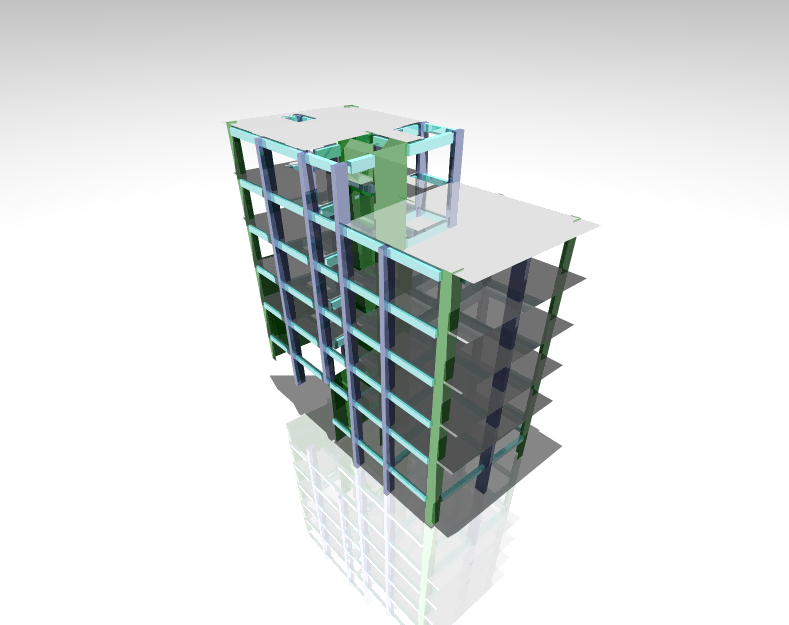
\includegraphics[scale=0.75]{IMAGENES/r2.png}
    \label{fig:my_label}
\end{figure}
\thispagestyle{empty}
\newpage

\clearpage                       % Otherwise \pagestyle affects the previous page.
{                                % Enclosed in braces so that re-definition is temporary.
  \pagestyle{empty}              % Removes numbers from middle pages.
  \fancypagestyle{plain}         % Re-definition removes numbers from first page.
  {
    \fancyhf{}%                       % Clear all header and footer fields.
    \renewcommand{\headrulewidth}{0pt}% Clear rules (remove these two lines if not desired).
    \renewcommand{\footrulewidth}{0pt}%
  }
    \begin{spacing}{1.35}
    \tableofcontents
  \end{spacing}
  \thispagestyle{empty}  
  \listoffigures
\newpage
\listoftables
  \thispagestyle{empty} 
% Removes numbers from last page.
}


%\listofmyequations
%\header{Realizado por: Alexis Pompilla Yábar}{}{}
\newpage
\begin{abstract}
\thispagestyle{empty}
El presente documento contempla todo lo concerniente al análisis y diseño estructural de la vivienda multifamiliar para acciones gravitacionales y sísmicas según lo establecido en el reglamento nacional de edificaciones vigente. De manera preliminar se presentan los datos de la edificación como la ubicación, planta y elevación arquitectónica, resultados y recomendaciones del estudio de mecánica de suelos. Posterior a esto se realiza la estructuración y el predimensionamiento de los elementos estructurales siguiendo lo establecido en las normas y recomendaciones de especialistas en la rama. Finalmente se realiza el análisis sísmico según la norma E-030, se verifica las irregularidades y se construye el espectro de respuesta de aceleraciones que representa la demanda sísmica, se realiza el análisis modal y se determina las dimensiones finales de los elementos para dotar al edificio de suficiente rigidez lateral para cumplir la deriva máxima permisible en estructuras de concreto armado, finalmente se verifica el sistema estructural y se escala las fuerzas obtenidas con el análisis dinámico modal espectral al porcentaje mínimo respecto a la cortante basal estática para combinar las fuerzas con las acciones gravitacionales según lo establecido en la norma E-060. La estructura resultante consiste en un sistema estructural de muros en la dirección X y de pórticos en la dirección Y, y derivas máximas de aproximadamente 0,0035 en la dirección X y 0.006 en Y. Finalmente se muestra el diseño por resistencia ultima de los elementos de concreto armado que conforma la edificación.
\vfill
\begin{flushleft}
\keywords{Vivienda multifamiliar, Análisis sísmico, E-030, E-060.}
\end{flushleft}

\end{abstract}
\newpage
\pagenumbering{arabic}
\section{Datos de la edificación}

% Table generated by Excel2LaTeX from sheet 'Hoja1'
\begin{table}[htbp]
  \centering
  %\caption{Add caption}
    \begin{tabular}{lrl}
    PROYECTO  & :     & CONSTRUCCION VIVIENDA MULTIFAMILIAR \\
          &       &  \\ 
    UBICACIÓN & :     & AV. CHINCHAYSUYO – AYUDA MUTUA Lt 03 Mz 03 \\
          &       &  \\
    DISTRITO & :     & CUSCO \\
          &       &  \\
    PROVINCIA & :     & CUSCO \\
          &       &  \\
    DEPARTAMENTO & :     & CUSCO \\
    \end{tabular}%
  \label{tab:addlabel}%
\end{table}%
\vspace{-0.8cm}

\section{Estudio de mecánica de suelos (EMS)}

\subsection{Perfil de suelo}

\begin{figure}[h!]
    \centering
    \caption{Clasificación del suelo}
    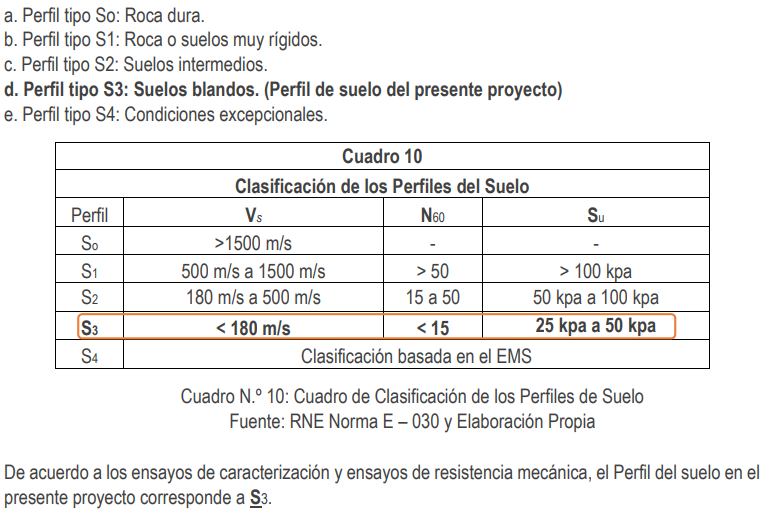
\includegraphics[scale=0.85]{IMAGENES/1.PNG}
    \caption*{\small Fuente: \it EMS}
    \label{fig:my_label}
\end{figure}

\newpage
\subsection{Profundidad de cimentación y capacidad portante}

\begin{figure}[h!]
    \centering
    \caption{Profundidad de cimentación}
    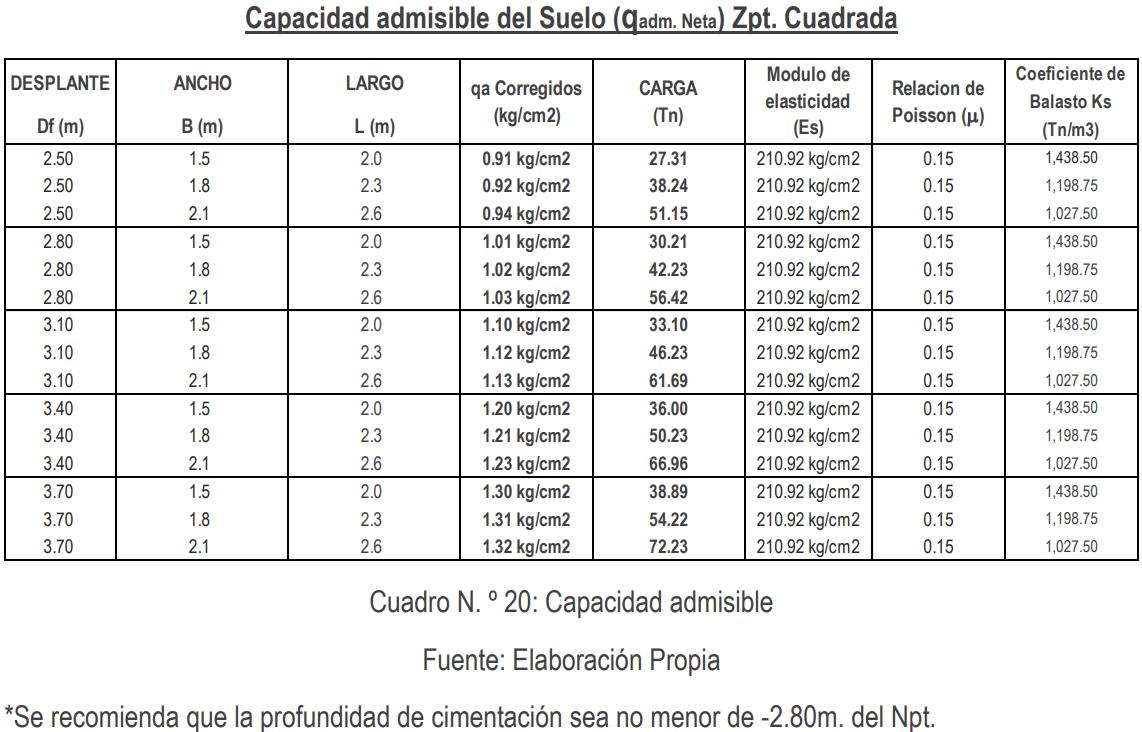
\includegraphics[scale=0.6]{IMAGENES/2.PNG}
    \caption*{\small Fuente: \it EMS}
    \label{fig:my_label}
\end{figure}

\section{Arquitectura}
Ver figuras \ref{pl} y \ref{el}.
\begin{figure}[h!]
    \centering
    \caption{Planta}
    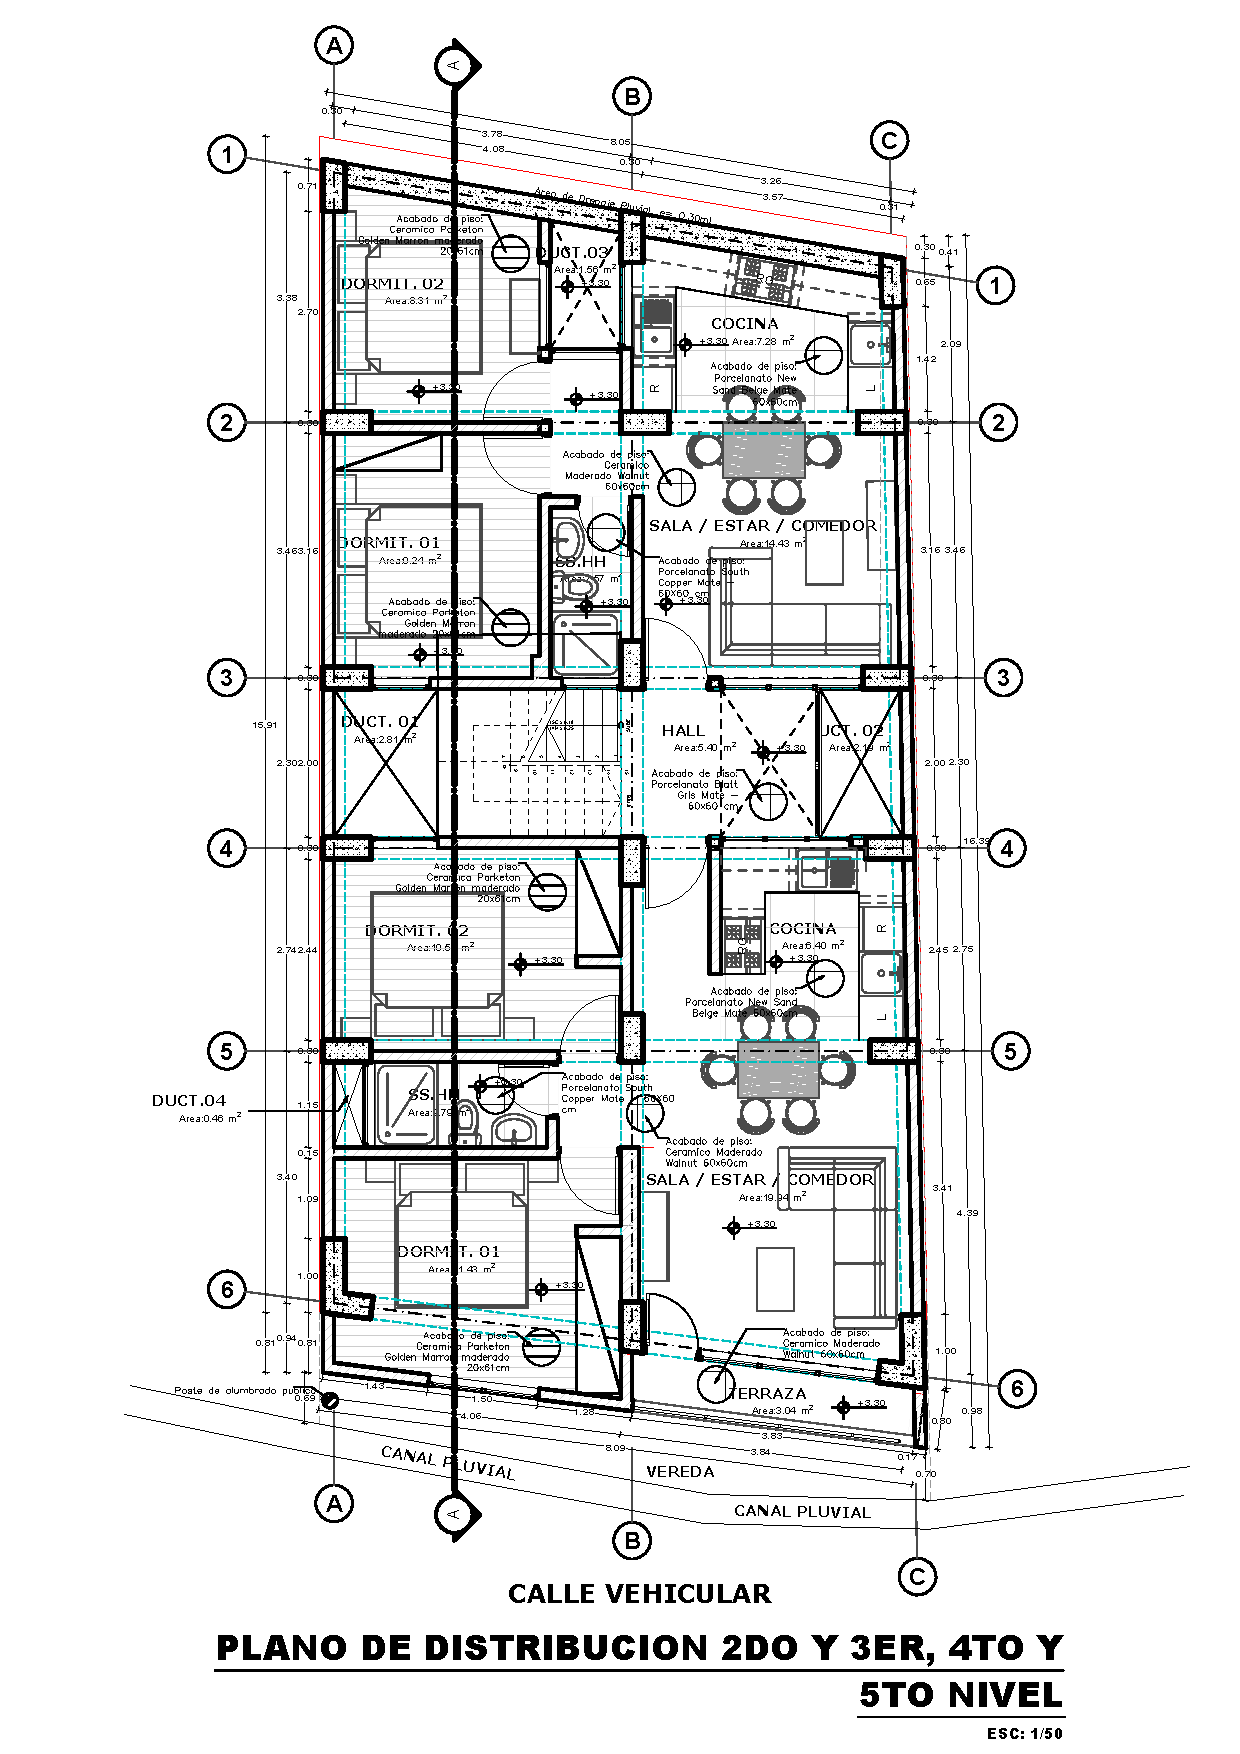
\includegraphics[scale=0.7]{IMAGENES/Plano.pdf}
    \label{pl}
\end{figure}

\begin{figure}[ht!]
    \centering
    \caption{Elevación}
    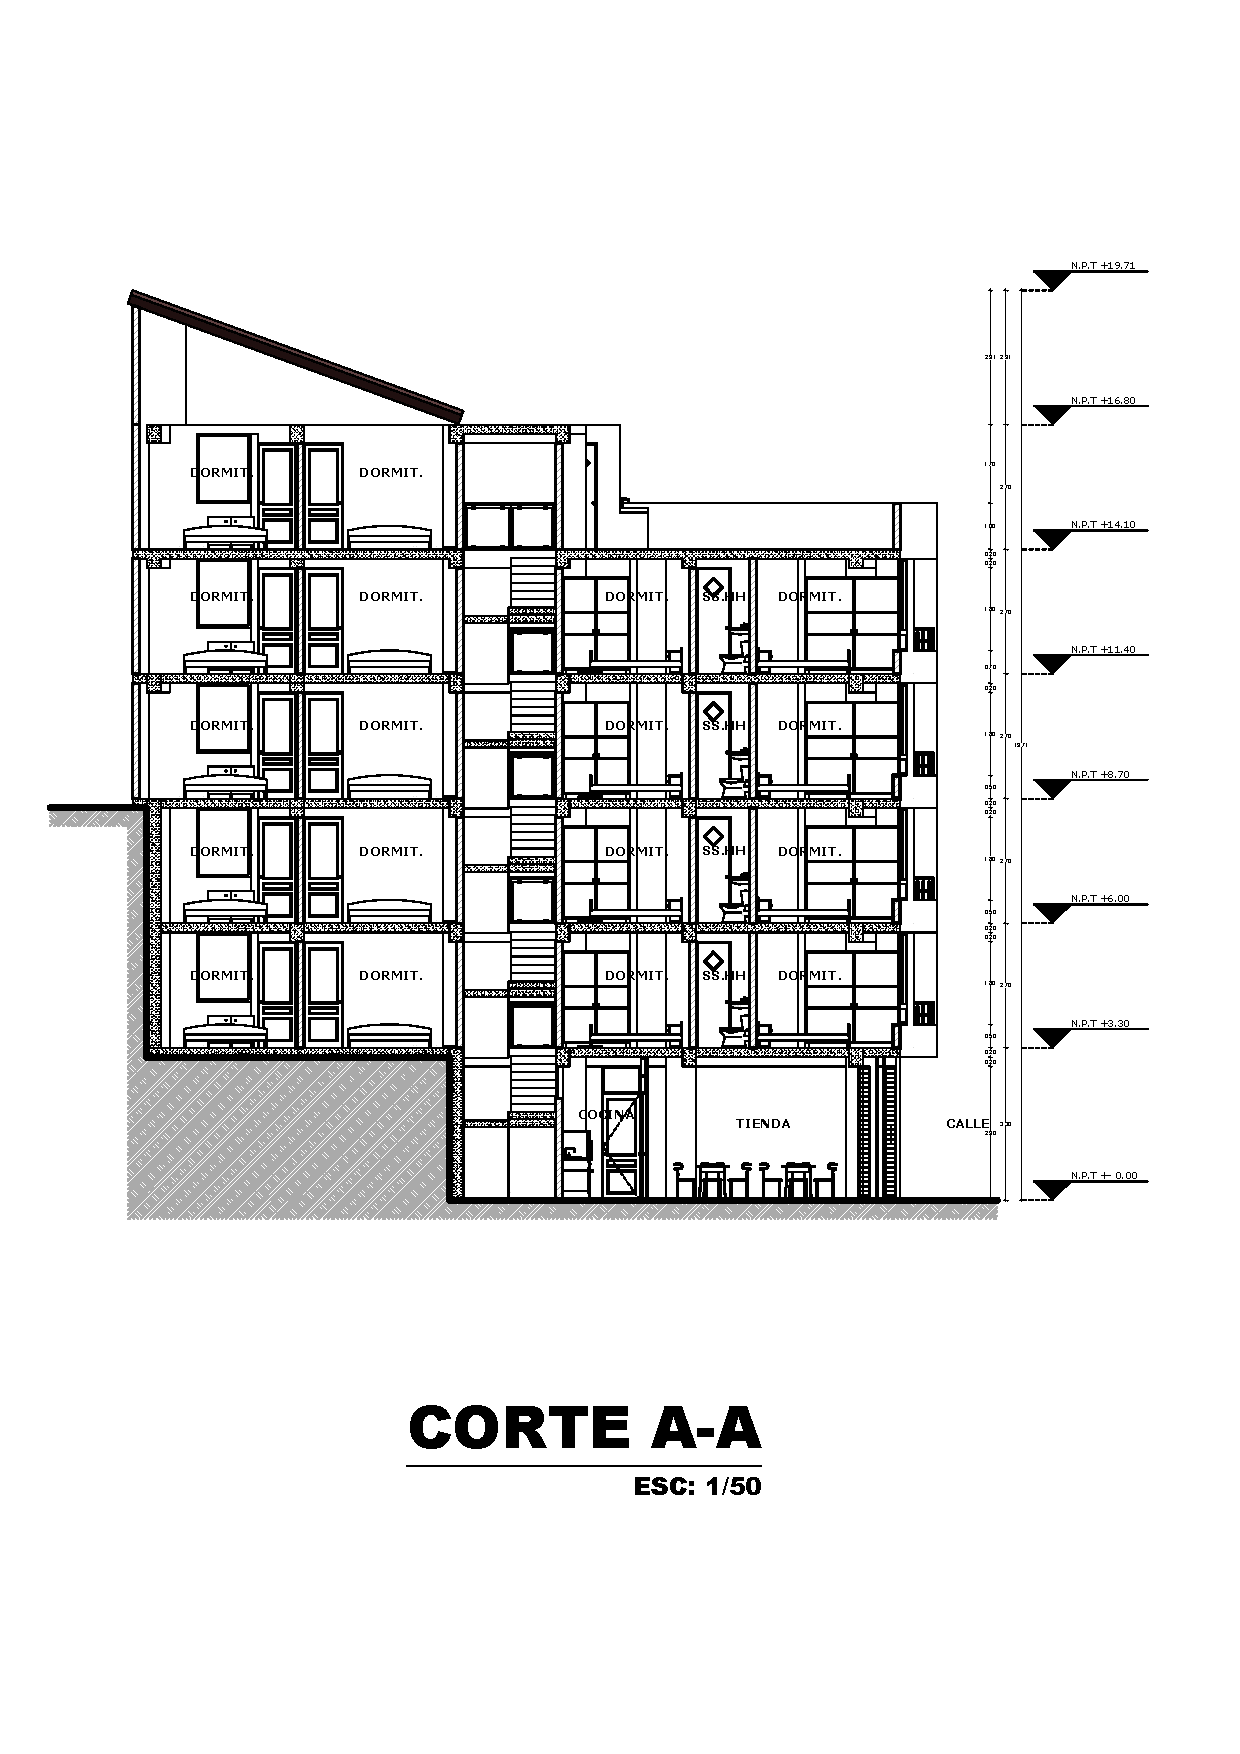
\includegraphics[trim={0 2cm 0 4.2cm},scale=0.7]{IMAGENES/ele.pdf}
    \label{el}
\end{figure}
%trim={<izquierda> <abajo> <derecha> <arriba>}
\section{Bases legales}
El desarrollo del presente trabajo se basa en las siguientes normas y reglamentos:
\begin{itemize}
  \item Norma Técnica de Edificación E.020 (Cargas)
  \item Norma Técnica de edificación E.030 (Diseño Sismoresistente)
  \item Norma Técnica de edificación E.050 (Suelos y Cimentaciones)
  \item Norma Técnica de edificación E.060 (Concreto Armado)
\end{itemize}
\section{Cargas de diseño}
Los cálculos y las consideraciones propias para el análisis con cargas de gravedad y de sismo, así como el diseño estructural del edificio se realizarán de acuerdo a lo especificado en las normas NTE E-020 Metrado de Cargas, NTE E-030 Diseño Sismorresistente, NTE E-060 Diseño de Concreto Armado.

\subsection{Cargas Muertas}

Las cargas muertas se determinan del cálculo directo del peso de todos los componentes estructurales y de elementos no estructurales cuya posición no se modificará durante la vida útil de la edificación. La norma E-020 del RNE nos proporciona algunos pesos unitarios para calcular la carga muerta, en nuestro caso tenemos:
\vspace{0.8cm}
% Table generated by Excel2LaTeX from sheet 'Hoja1'
\begin{table}[htbp]
  \centering
 % \caption{Add caption}
    \begin{tabular}{lrl}
    Concreto armado & :     & 2400 kg/m\raisebox{1ex}{\scriptsize{3}}\\
              &       &  \\
    Muro de albañilería hueca & :     & 1350 kg/m\raisebox{1ex}{\scriptsize{3}} \\
              &       &  \\
    Muro de albañilería solida                              & :     & 1800 kg/m\raisebox{1ex}{\scriptsize{3}}  \\
              &       &  \\
    Mortero de cemento & :     & 2000 kg/m\raisebox{1ex}{\scriptsize{3}}  \\
              &       &  \\
    Piso terminado (pt)  & :     & 100 kg/m\raisebox{1ex}{\scriptsize{2}}  \\
    \end{tabular}%
  \label{tab:addlabel}%
\end{table}%

La carga muerta lo calcula el programa, pero adicionalmente se consideró una sobrecarga permanente de 100 kg/m\raisebox{1ex}{\scriptsize{2}} que incluye piso terminado.
También se incluyó las cargas distribuidas directamente sobre vigas debido a las tabiquerías de espesor 15 cm. Los muros se suponen construidos con ladrillos pandereta cuyo peso especifico se extrae de la norma E-020:

\begin{figure}[h!]
    \centering
    \caption{Peso unitario de tabiquería}
    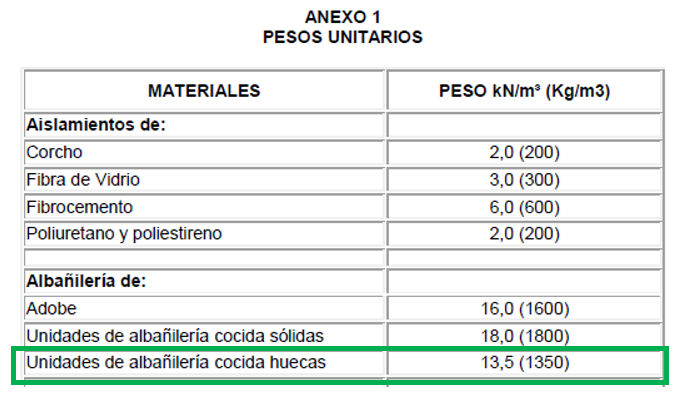
\includegraphics[scale=0.7]{IMAGENES/3.PNG}
    \caption*{\small Fuente: \it \cite{E-020}}
    \label{fig:my_label}
\end{figure}

\newpage

\subsection{Cargas Vivas}
La carga de piso que se va aplicar a un área determinada de una edificación depende de su pretendida utilización u ocupación. Estas cargas se deben a los seres humanos, al equipo, al almacenamiento en general, a los automóviles, etc., debido a que estas cargas son de naturaleza aleatoria, no hay una forma precisa para aplicar las cargas reales a un área dada. Por esa razón se especifican como cargas distribuidas uniformemente en el área. Cabe indicar que estas cargas son extremamente conservadoras debido a la incertidumbre acerca de cómo pudieran distribuirse las cargas reales. La norma E020 nos da cargas distribuidas para distintos tipos de ocupación o uso, en nuestro caso para una edificacion de vivienda se tiene:  

\begin{figure}[h]
    \centering
    \caption{Carga viva para viviendas}
    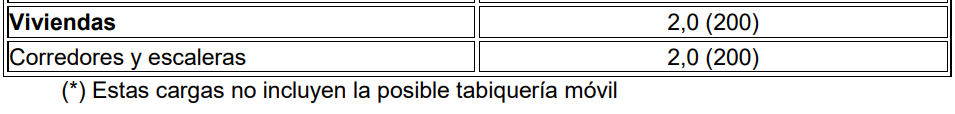
\includegraphics[scale=0.8]{IMAGENES/4.PNG}
    \label{fig:my_label}
    \caption*{\small Fuente: \it \cite{E-020}}
\end{figure}

\begin{figure}[h]
    \centering
    \caption{Carga viva en azoteas}
    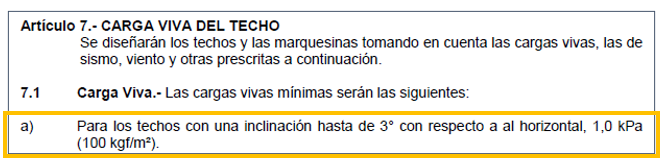
\includegraphics[scale=1]{IMAGENES/7.PNG}
    %\label{fig:my_label}
    \caption*{\small Fuente: \it \cite{E-020}}
\end{figure}

\newpage
\section{Propiedades del material}

Dado que se trata de un análisis lineal elástico las únicas propiedades que involucran en el calculo son las del concreto y se extraen de la \cite{E-060}:
\vspace{0.5cm}
% Table generated by Excel2LaTeX from sheet 'Hoja1'
\begin{table}[htbp]
  \centering
 % \caption{Add caption}
    \begin{tabular}{>{\arraybackslash}m{7cm}>{\arraybackslash}m{0.2cm}>{\arraybackslash}m{8cm}}
    $\bullet$ Resistencia máxima a la compresión  & :     & $f' _{c}=210$ kg/cm\raisebox{1ex}{\scriptsize{2}} \\
              &       &  \\
   % $\bullet$ Deformación unitaria máxima  & :     & $\varepsilon _{c}=0.003$ \\
   %           &       &  \\
    $\bullet$ Módulo de Elasticidad  & :     & $E _{c}=15000\;f'_{c}=217,370.65
    $ kg/cm\raisebox{1ex}{\scriptsize{2}} \\
              &       &  \\
    $\bullet$ Relación entre módulos de elasticidad & :     & $E _{c}/G=2.3$ \\
    \end{tabular}%
  \label{tab:addlabel}%
\end{table}%
\section{Estructuracion}
Según \cite{san1998analisis}, la estructuración de un edificio consiste en “tomar decisiones en conjunto con los otros profesionales que intervienen en la obra acerca de la disposición y características que deben tener los diferentes elementos estructurales, de manera que el edificio tenga un buen comportamiento durante su vida útil; esto es, que tanto las cargas permanentes (peso propio, acabados, etc.) como las eventuales (sobrecarga, sismo, viento, etc.), y se transmitan adecuadamente hasta el suelo de cimentación”.\\
\section{Predimensionamiento}
\subsection{Losas Aligeradas}
Según \cite{blanco} el peralte de las losas aligeradas podrá ser dimensionado considerando los siguientes criterios:
\newpage
\begin{table}[htbp]
  \centering
  \caption{Peso propio y espesores recomendados en aligerados}
  \vspace{0.15cm}
{
\extrarowheight = -0.5ex
\renewcommand{\arraystretch}{1.8}

\begin{tabular}{|>{\centering\arraybackslash}m{2cm}|>{\centering\arraybackslash}m{5cm}| >{\centering\arraybackslash}m{5cm}|}
 %\begin{tabular}{|c|c|c|}
    \hline
    \textbf{h (m)} & 
    \textbf{Peso propio aproximado (kg/m\raisebox{1ex}{\scriptsize{2}})} & 
    \textbf{Luces máximas recomendadas (m)} \\
    \hline
    0.17  & 280   & ln $\leq$ 4 \\
    0.20   & 300   & 4 $\leq$ ln $\leq$ 5.5 \\
    0.25  & 350   & 5.5 $\leq$ ln $\leq$ 6.6 \\
    0.30   & 420   & 6 $\leq$ ln $\leq$ 7.5 \\
    \hline
 \end{tabular}%
}
  \caption*{\small Fuente: \it \cite{blanco}}
  \label{tab:addlabel}%
\end{table}%
\noindent
Se entiende por h al espesor total del aligerado incluyendo los 5cm de losa superior.
\\
El criterio anterior sólo aplica para sobrecargas máximas de 300 a 350 kg/m\raisebox{1ex}{\scriptsize{2}}.
\\
Teniendo en cuenta estos criterios se adopto losas aligeradas armadas en el sentido paralelo a los ejes A,B y C. El espesor entre los ejes 1 y 3 es de 17cm y entre los ejes 4 y 6 es de 20cm.

\subsection{Losas Macizas}
Se adopto una losa maciza en la zona donde existe discontinuidad del diafragma debido a los ductos y la presencia de la escalera. Se adopto un peralte de 20cm con la intención de trasmitir las fuerzas sísmicas del diafragma adecuadamente a los demás elementos.

\subsection{Vigas principales}
Se provee al edificio de vigas peraltadas en las dos direcciones ``X'' e ``Y'', a manera de contar con suficiente rigidez lateral ante un evento sísmico y trabajen de manera conjunta como pórtico y/o pórtico-placa.
\\
Según \cite{blanco}, las vigas se dimensionan generalmente considerando un peralte del orden de 1/10 a 1/12 de la luz libre.
\\
Las vigas dimensionadas con este criterio son diseñadas solo con acero en tracción y no existe problemas de deflexiones grandes.
La norma peruana E 060 indica que el ancho mínimo de vigas que forman parte de elementos sismorresistentes debe ser 25cm.
\\
Las luces libres de máxima longitud son de aproximadamente de 4m por lo que según este criterio solo sería necesario peraltes del orden de 40cm, sin embargo, después de realizar el análisis sísmico se adoptó vigas principales de 30x50cm para cumplir con los requisitos que se mencionan posteriormente.

\subsection{Vigas secundarias}
Al igual que en el caso anterior las dimensiones finales de las vigas secundarias son por requerimiento de rigidez lateral resultando estas 25x40cm.

\subsection{Columnas}

Según \cite{ovi2016} las dimensiones de las columnas se pueden estimar con la expresión:

\begin{equation}
A_{c}=\frac{\lambda\;P_{g} }{\eta \;f'_{c}}
\end{equation}
\myequations{Predimensonamiento de columnas}

\begin{flushleft}
Donde:\\
$\lambda$, $\eta$ = Factores obtenidos de la tabla .\\
$P_{g}$ = Carga gravitacional repartida por m\raisebox{1ex}{\scriptsize{2}}, se puede asumir 1 ton/m\raisebox{1ex}{\scriptsize{2}}\\
$f'_{c}$ = Resistencia a compresión del concreto.\\
\end{flushleft}

% Table generated by Excel2LaTeX from sheet 'Hoja1'
\begin{table}[htbp]
  \centering
  \caption{Predimensionamiento de columnas}
    \begin{tabular}{|c|c|c|}
    \hline
    \rowcolor[rgb]{ .906,  .902,  .902} \textit{\textbf{Tipo de columna:}} & \multicolumn{1}{p{10.665em}|}{\centering\textbf{$\lambda$}} & \multicolumn{1}{p{11.945em}|}{\centering\textbf{$\eta$}} \\
    \hline
    \rowcolor[rgb]{ .906,  .902,  .902} Central & \cellcolor[rgb]{ 1,  1,  1}1.10 & \cellcolor[rgb]{ 1,  1,  1}0.30 \\
    \hline
    \rowcolor[rgb]{ .906,  .902,  .902} Perimetral & \cellcolor[rgb]{ 1,  1,  1}1.25 & \cellcolor[rgb]{ 1,  1,  1}0.25 \\
    \hline
    \rowcolor[rgb]{ .906,  .902,  .902} Esquinera & \cellcolor[rgb]{ 1,  1,  1}1.50 & \cellcolor[rgb]{ 1,  1,  1}0.20 \\
    \hline
    \end{tabular}%
  \label{tab:addlabel}%
\end{table}%

Después de aplicar la ecuación  para la columnas con mayor área tributaria se obtuvo dimensiones mínimas, sin embargo las dimensiones finales de las columnas son por requerimiento de rigidez lateral, resultado estas de 30x65 peraltadas en la dirección paralela al eje X.


\subsection{Muros de corte o placas}

La longitud final de los muros en ambas direcciones se establece después de realizar un análisis sísmico iterativo hasta cumplir con los requisitos de rigidez lateral de la norma E-030.
\section{Modelamiento}

El modelo matemático se construyo en el software de análisis y diseño estructural ETABS en su versión 20.1.1, el material se definió según lo mencionado en el inciso 7 del presente documento, las secciones se crearon según lo mencionado en el predimensionamiento. Para el modelado de losas y muros se utilizo elementos shell y para columnas y vigas se utilizo elementos frame, sin embargo cuando existe columnas que forman parte de algún muro estos se modelaron con elementos shell para integrar de mejor manera los esfuerzos resultantes, asi mismo se aseguro un correcto mesh en esos elementos para poder capturar el comportamiento a flexion. 
\\
Las alturas de entrepiso se tomaron según los planos de arquitectura, la profundidad de cimentación se considero de 3.10m y las columnas y muros se modelaron hasta la cara superior de la cimentación, para lo cual se estimo un espesor de la zapata o platea de 0.6m. 
\\
Las zonas de los nudos de columnas y vigas se modelaron con un factor de rigidez del 50 \%, se consideran las rigideces brutas de los elementos como se menciona en la E-030 a excepción de las losas donde se redujo la rigidez axial, a flexión y a cortante a un 25 \% según lo mencionado en \cite{ACI19}. Debido a las aberturas y la relación de dimensiones de la planta del edificio no se considera un diafragma rígido en los sistemas de piso.
\\
\newpage

\newsavebox\mybox
\savebox{\mybox}{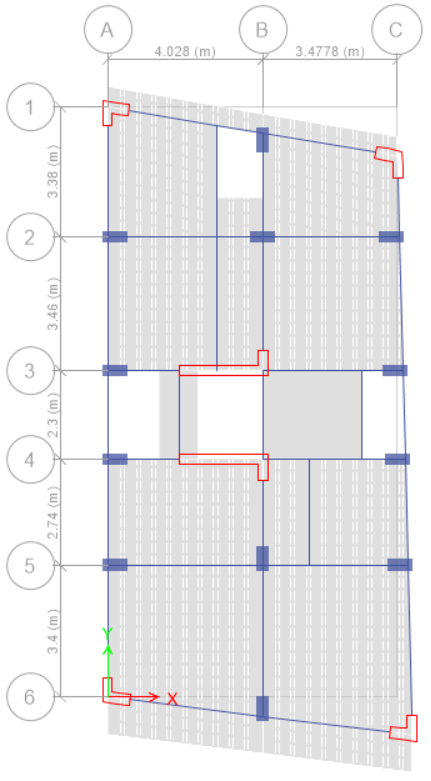
\includegraphics[width=7cm]{IMAGENES/6.PNG}}
\begin{figure}[h]
    \centering
    \begin{minipage}{0.45\textwidth}
        \centering
        \usebox{\mybox}
        \caption{Planta típica}
    \end{minipage}
    \begin{minipage}{0.45\textwidth}
        \centering
        \vbox to \ht\mybox{%
            \vfill
            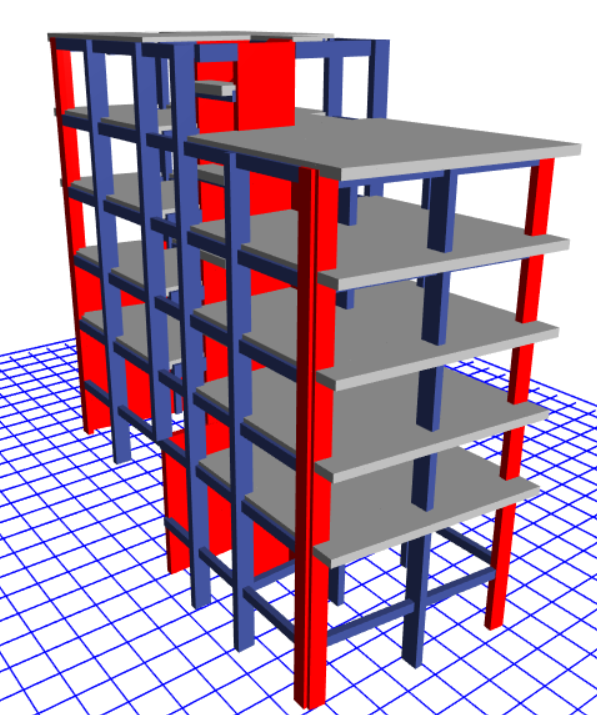
\includegraphics[width=7cm]{IMAGENES/5.PNG}
            \vfill
        }
        \caption{Vista 3D}
    \end{minipage}
\end{figure}
\section{Análisis Sísmico}
\subsection{Parámetros de sitio}
\subsubsection{Zonificación}
La ubicación de este proyecto es en la ciudad de Cusco, en el distrito de Cusco. Siguiendo los parámetros de la norma de diseño sismorresistente E.030 de octubre de 2018, la estructura se encuentra en la Zona 2. Por ello que el factor que se interpreta como la aceleración máxima horizontal en el suelo rígido con una probabilidad de 10 \% de ser excedida en 50 años es igual a \textbf{0.25}.
\newpage
%\vspace{-10cm}
\begin{table}[ht!]
    \centering
    \begin{minipage}{0.55\textwidth}
    \vspace{-4cm}
    \caption{Factor de zona}
    \begin{tabular}{|>{\centering\arraybackslash}m{3.75cm}|>{\centering\arraybackslash}m{3.75cm}|}
    \hline
    \multicolumn{2}{|c|}{\textbf{FACTOR DE ZONA SEGÚN E-030}} \\
    \hline
    \textit{\textbf{ZONA}} & \textit{\textbf{Z}} \\
    \hline
    4     & 0.45 \\
    \hline
    3     & 0.35 \\
    \hline
    \rowcolor[rgb]{ .949,  .949,  .949} 2     & \textcolor[rgb]{ 1,  0,  0}{\textbf{0.25}} \\
    \hline
    1     & 0.10 \\
    \hline
    \end{tabular}%
    \end{minipage}
    \begin{minipage}{0.35\textwidth}
    \vspace{-4cm}
        \centering
        \vbox to \ht\mybox{%
            \vfill
            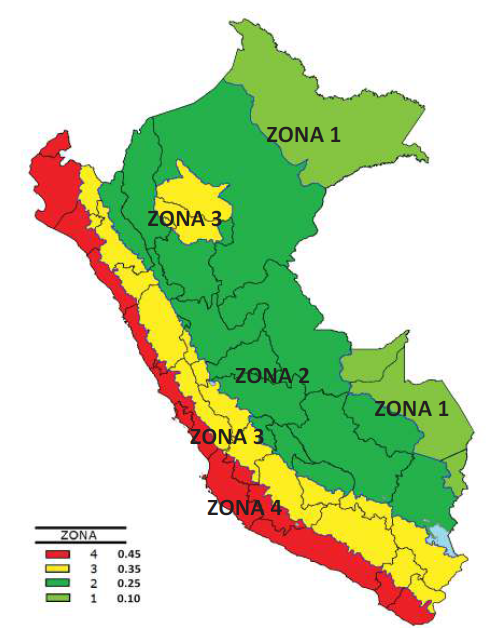
\includegraphics[width=4cm]{IMAGENES/8.png}
            \vfill
        }
    \end{minipage}
    \vspace{-3.5cm}
    \caption*{\small Fuente: \it \cite{E-030}}
\end{table}
%\vspace{-3.5cm}
\subsubsection{Factor de suelo}
%\vspace{-4cm}
% Table generated by Excel2LaTeX from sheet '00-d) Parametros sismicos'
\begin{table}[h!]
  \centering
  \caption{Factor de suelo}
    \begin{tabular}{|>{\centering\arraybackslash}m{3.75cm}|>{\centering\arraybackslash}m{2cm}|>{\centering\arraybackslash}m{2cm}|>{\centering\arraybackslash}m{2cm}|>{\centering\arraybackslash}m{2cm}|}
    \hline
    \multicolumn{5}{|c|}{\textbf{FACTOR DE SUELO SEGÚN E-030}} \\
    \hline
    \backslashbox{\textit{\textbf{ZONA}}}{\textit{\textbf{SUELO}}} & \textit{\textbf{S0}} & \textit{\textbf{S1}} & \textit{\textbf{S2}} & \textit{\textbf{S3}} \\
    \hline
    \textit{\textbf{4}} & 0.80  & 1.00  & 1.05  & \cellcolor[rgb]{ .949,  .949,  .949}1.10 \\
    \hline
    \textit{\textbf{3}} & 0.80  & 1.00  & 1.15  & \cellcolor[rgb]{ .949,  .949,  .949}1.20 \\
    \hline
    \rowcolor[rgb]{ .949,  .949,  .949} \textit{\textbf{2}} & 0.80  & 1.00  & 1.20  & \textcolor[rgb]{ 1,  0,  0}{\textbf{1.40}} \\
    \hline
    \textit{\textbf{1}} & 0.80  & 1.00  & 1.60  & \cellcolor[rgb]{ .949,  .949,  .949}2.00 \\
    \hline
    \end{tabular}%
    \caption*{\small Fuente: \it \cite{E-030}}
  \label{tab:addlabel}%
\end{table}%

\subsubsection{Periodos de suelo}
% Table generated by Excel2LaTeX from sheet '00-d) Parametros sismicos'
\begin{table}[h!]
  \centering
  \caption{Periodos de suelo}
    \begin{tabular}{|>{\centering\arraybackslash} m{2cm}|>{\centering\arraybackslash}m{2cm}|>{\centering\arraybackslash}m{2cm}|>{\centering\arraybackslash}m{2cm}|>{\centering\arraybackslash}m{2cm}|}
\cline{2-5}     \multicolumn{1}{r|}{} & \multicolumn{4}{c|}{\textbf{PERIODO "Tp" y "Tl" SEGÚN E-030}} \\
\cline{2-5}     \multicolumn{1}{r|}{} & \multicolumn{4}{c|}{\textit{\textbf{Perfil de suelo}}} \\
\cline{2-5}     \multicolumn{1}{r|}{} & \textit{\textbf{S0}} & \textit{\textbf{S1}} & \textit{\textbf{S2}} & \textit{\textbf{S3}} \\
    \hline
    \textit{\textbf{Tp}} & 0.30  & 0.40  & 0.60  & \cellcolor[rgb]{ .949,  .949,  .949}\textcolor[rgb]{ 1,  0,  0}{\textbf{1.00}} \\
    \hline
    \textit{\textbf{Tl}} & 3.00  & 2.50  & 2.00  & \cellcolor[rgb]{ .949,  .949,  .949}\textcolor[rgb]{ 1,  0,  0}{\textbf{1.60}} \\
    \hline
    \end{tabular}%
    \caption*{\small Fuente: \it \cite{E-030}}
  \label{tab:addlabel}%
\end{table}%

\subsection{Sistema Estructural}
Después de realizar el análisis sísmico se determino que los sistemas estructurales en X, Y son de muros y pórticos respectivamente.
% Table generated by Excel2LaTeX from sheet '00-d) Parametros sismicos'
\begin{table}[h!]
  \centering
  \caption{coeficiente básico de reducción }
    {
\extrarowheight = -0.3ex
\renewcommand{\arraystretch}{1.4}
    \begin{tabular}{|>{\arraybackslash}m{10cm}| >{\centering\arraybackslash}m{4cm}|}
    \hline
    \multicolumn{2}{|c|}{\textbf{SISTEMAS ESTRUCTURALES }} \\
    \hline
    \textit{\textbf{Sistema Estructural}} & \multicolumn{1}{m{4cm}|}{\textit{\textbf{Coeficiente Básico de Reducción Ro}}} \\
    \hline
    \multicolumn{2}{|l|}{\textbf{Acero:}} \\
    \hline
    Porticos Especiales Resistentes a Momento (SMF) & 8 \\
    \hline
    Porticos Intermedios Resistentes a Momento (IMF) & 5 \\
    \hline
    Porticos Ordinarios Resistentes a Momento (OMF) & 4 \\
    \hline
    Porticos Especiales Concentricamente Arrriostrados (SCBF) & 7 \\
    \hline
    Porticos Ordinarios Concentricamente Arrriostrados (OCBF) & 4 \\
    \hline
    Porticos Excentricamente Arriostrados (EBF) & 8 \\
    \hline
    \multicolumn{2}{|l|}{\textbf{Concreto Armado:}} \\
    \hline
    \rowcolor[rgb]{ .906,  .902,  .902} Porticos & \textcolor[rgb]{ 1,  0,  0}{\textbf{8}} \\
    \hline
     Dual  & 7 \\
    \hline
    \rowcolor[rgb]{ .906,  .902,  .902} De muros estructurales & \textcolor[rgb]{ 1,  0,  0}{\textbf{6}} \\
    \hline
    Muros de ductilidad limitada & 4 \\
    \hline
    \textbf{Albañilería Armada o Confinada} & 3 \\
    \hline
    \textbf{Madera} & 7 \\
    \hline
    \end{tabular}%
    }
    \caption*{\small Fuente: \it \cite{E-030}}
  \label{tab:addlabel}%
\end{table}%
\vspace{-0.8cm}

\subsection{Factor de amplificación sísmica}
Se determina según el articulo 11 de la E-030.
\newpage
%\newpage
\setlength{\jot}{0.5cm}% Inter-equation spacing
\begin{figure}[h!]
    \centering
    \begin{minipage}{0.5\textwidth}
    \vspace{-4cm}
    \caption{Factor de amplificación}
        \begin{align*}
        &T< T_{P}         &   C&=2,5\cdot\left ( \frac{T_{P}}{T} \right )\\
        &T_{P}< T< T_{L}  &   C&=2,5\cdot\left ( \frac{T_{P}}{T} \right )\\
        &T> T_{L}         &   C&=2,5\cdot\left ( \frac{T_{P}\;T_{L}}{T^{2}} \right )
        \end{align*}
    \end{minipage}
    \begin{minipage}{0.4\textwidth}
    \vspace{-3cm}
        \centering
        \vbox to \ht\mybox{%
            \vfill
            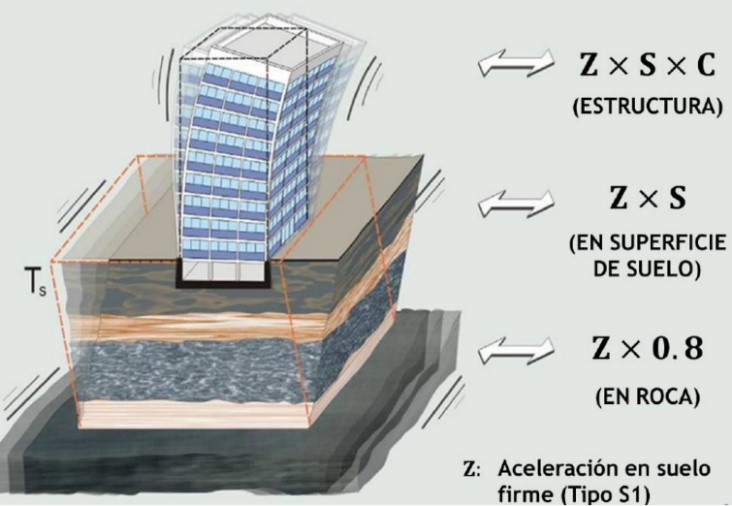
\includegraphics[width=6.5cm]{IMAGENES/9.jpg}
            \vfill
       }
    \end{minipage}
    \vspace{-3.4cm}
    \caption*{\small Fuente: \it \cite{comen}}
  \label{fac}
\end{figure}
\vspace{-0.8cm}
\subsection{Factor de importancia}
% Table generated by Excel2LaTeX from sheet '00-d) Parametros sismicos'
\begin{table}[h!]
  \centering
  \caption{Factor de Uso o importancia}
    \begin{tabular}{|>{\arraybackslash}m{3cm}|m{8cm}|>{\arraybackslash}m{2.8cm}|}
    \hline
    \multicolumn{3}{|c|}{\textbf{CATEGORIA DE LA EDIFICACION}} \\
    \hline
    \multicolumn{1}{|c|}{\textit{\textbf{CATEGORIA}}} & \multicolumn{1}{c|}{\textit{\textbf{DESCRIPCION}}} & \multicolumn{1}{c|}{\textit{\textbf{FACTOR U}}} \\
    \hline
    \multirow{2}[4]{3cm}{A Edificaciones Escenciales} & A1: Establecimiento del sector salud (públicos y privados) del segundo y tercer nivel, según lo normado por el ministerio de salud. & Con aislamiento 1.0 y sin aislamiento 1.5. \\
\cline{2-3}    \multicolumn{1}{|c|}{} & A2: Edificaciones escenciales para el manejo de las emergencias, el funcionamiento del gobierno y en general aquellas que puedan servir de refugio después de un desastre. & \multicolumn{1}{c|}{1.50} \\
    \hline
    B Edificaciones Importantes & Edificaciones donde se reúnen gran cantidad de personas tales como cines, teatros, estadios, coliseos, centros comerciales, terminales de buses de pasajeros, establecimientos penitenciarios, o que guardan patrimonios valiosos como museos y bibliotecas. & \multicolumn{1}{c|}{1.30} \\
    \hline
    \rowcolor[rgb]{ 1,  .949,  .8} C Edificaciones Comunes & Edificaciones comunes tales como: viviendas, oficinas, hoteles, restaurantes, depósitos e instalaciones industriales cuya falla no acarree peligros adicionales de incendios o fugas de contaminantes. & \multicolumn{1}{c|}{\textcolor[rgb]{ 1,  0,  0}{\textbf{1.00}}} \\
    \hline
    D Edificaciones temporales & Construcciones provisionales para depósitos, casetas y otras similares. & A criterio del proyectista \\
    \hline
    \end{tabular}%
    \caption*{\small Fuente: \it \cite{E-030}}
  \label{tab:addlabel}%
\end{table}%


\newpage


% Table generated by Excel2LaTeX from sheet '07) ESPECTRO FINAL'
\begin{table}[htbp]
  \centering
  \caption{Resumen de parámetros sísmicos}
  {
\extrarowheight = -0.3ex
\renewcommand{\arraystretch}{1.5}
    \begin{tabular}{m{5cm}|>{\centering\arraybackslash}m{2cm}|>{\centering\arraybackslash}m{2cm}|>{\centering\arraybackslash}m{2cm}|}
\cline{2-4}          & \multicolumn{3}{c|}{\textbf{PARAMETROS SISMICOS}} \\
\cline{2-4}          &       & \textit{\textbf{X}} & \textit{\textbf{Y}} \\
\cline{2-4}  \multicolumn{1}{l|}{\textit{Factor de Zona (Tabla N°1)}} & \textbf{Z} & \multicolumn{2}{c|}{0.25} \\
\cline{2-4}    \multicolumn{1}{l|}{\textit{Factor de Uso (Tabla N°5)}} & \textbf{U} & \multicolumn{2}{c|}{1.00} \\
\cline{2-4}    \multicolumn{1}{l|}{\textit{Factor de Suelo (Tabla N°3)}} & \textbf{S} & \multicolumn{2}{c|}{1.40} \\
\cline{2-4}    \multicolumn{1}{l|}{\multirow{2}{*}{\textit{Periodos (Tabla N°4)}}} & \textbf{T\raisebox{-0.5ex}{\scriptsize{P}}} & \multicolumn{2}{c|}{1.00} \\
\cline{2-4}          & \textbf{T\raisebox{-0.5ex}{\scriptsize{L}}} & \multicolumn{2}{c|}{1.60} \\
\cline{2-4}    \multicolumn{1}{l|}{\textit{Coef. Básico de Reducción (Tabla N°7)}} & \textbf{R\raisebox{-0.5ex}{\scriptsize{o}}} & 6.00  & 8.00 \\
\cline{2-4}    \multicolumn{1}{l|}{\textit{Irregularidad en altura (Tabla N°8)}} & \textbf{I\raisebox{-0.5ex}{\scriptsize{a}}} & 1.00  & 1.00 \\
\cline{2-4}    \multicolumn{1}{l|}{\textit{Irregularidad en planta (Tabla N°9)}} & \textbf{I\raisebox{-0.5ex}{\scriptsize{p}}} & 1.00  & 1.00 \\
\cline{2-4}    \multicolumn{1}{l|}{\textit{Coef. de Reducción (Articulo 22)}} & \textbf{R} & 6.00  & 8.00 \\
\cline{2-4}          & \textbf{ZUSg/R} & 0.57  & 0.43 \\
\cline{2-4}    \end{tabular}%
}
  \label{tab:addlabel}%
\end{table}%

\subsection{Espectro de respuesta de aceleraciones}
\begin{figure}[h!]
    \centering
    \begin{tikzpicture}
    %draw[color=blue, help lines,dashed ] (0,0) grid (4.5,1.7);
    \begin{axis}
    [grid=both,
    grid style={line width=.1pt,dashed, draw=gray!10},
    major grid style={line width=.2pt,draw=gray!50},name=plot, xlabel={T (s)},ylabel={Sa (m/s2)},xmin=0,xmax=4,
    ymin=0,ymax=1.7,width=.8\textwidth,height=10cm,legend entries={X (R=6),Y(R=8)},legend pos=north east]%,xtick distance=.5%,ytick distance=.5]
    \addplot[OrangeRed,ultra thick] table{DATOS/EX6.txt};\label{xx}
    \addplot[MidnightBlue,ultra thick] table{DATOS/EY8.txt};\label{yy}
    %\addplot[black,mark=triangle*] table{./espectro R=8.txt};\label{f}
    %\addplot[red,mark=o] table{./data/generator.txt};\label{g}
    %\addplot[blue] table{./data/simulated_total.txt};\label{s}
    %\addplot[green,dashed] table{./data/theoretical_total.txt};\label{t}
% Define two points for drawing an arrow to the "matched" point
    \node[] (C) at (axis cs: 1,1.6) {\hspace{0.5cm}Tp};
    \node[] (B) at (axis cs: 1,0) {};
    \node[] (D) at (axis cs: 1.6,1.6) {\hspace{0.5cm}Tl};
    \node[] (G) at (axis cs: 1.6,0) {};
    \end{axis}
 % Create a node to act as the legend  
    %\node[anchor=north,fill=white,draw=black] (legend) at ($(plot.north)-(-28 mm, 8.5 mm)$) {\begin{tabular}{l l l l}
       % X (R=6) & \ref{xx}\\ % & Y (R=8) & \ref{yy} \\
       % Y (R=8) & \ref{yy}\\ % & Y (R=8) & \ref{yy} \\
        %s & \ref{s}  & t & \ref{t} \\
   % \end{tabular} };

%\draw [dashed] (10,1) -- (10,11);
\draw[dashed,color=green,line width=1pt] (C)--(B);
\draw[dashed,color=orange,line width=1pt] (D)--(G);
%\node[anchor=west] (label) at (B) {matched};
    
    \end{tikzpicture}
    \caption{Espectro de aceleraciones}
    \label{fig:my_label}
\end{figure}


\subsection{Peso Sísmico}
\begin{mybox3}{Art. 23 E-030}
\textit{El peso (P), se calcula adicionando a la carga permanente y total de la edificación un porcentaje de la carga viva o sobrecarga. En edificaciones de la categoría C, se toma el 25\% de la carga viva.}
\end{mybox3}

\subsection{Excentricidad Accidental}

\begin{mybox3}{Art. 26.5 E-030}
\textit{La incertidumbre en la localización de los centros de masa en cada nivel, se considera mediante una excentricidad accidental perpendicular a la dirección del sismo igual a 0,05 veces la dimensión del edificio en la dirección perpendicular a la dirección de análisis. En cada caso se considera el signo más desfavorable.}
\end{mybox3}
\noindent
Para determinar el sentido mas desfavorable de la excentricidad accidental se calculo el centro de masa y centro de rigidez del edificio, resultando negativo en ambos casos, la excentricidad se asigna a la masa como se muestra en la figura \ref{masa} .

\begin{figure}[h!]
    \centering
    \caption{Excentricidad de la masa en ETABS}
    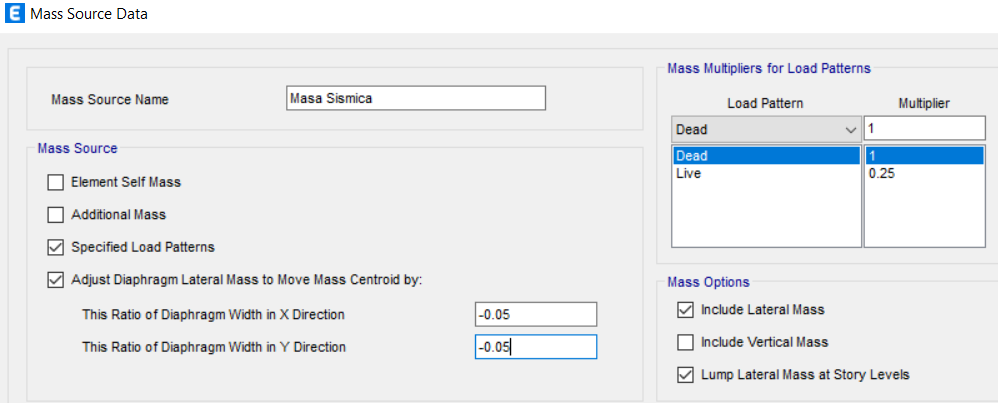
\includegraphics[scale=0.7]{IMAGENES/15.PNG}
    \label{masa}
\end{figure}

\newpage
\subsection{Análisis modal Art. 26.1 E-030}

\begin{mybox3}{Art. 26.1.1}
\textit{Los modos de vibración pueden determinarse por un procedimiento de análisis que considere apropiadamente las características de rigidez y la distribución de las masas.}
\end{mybox3}

\begin{mybox3}{Art. 26.1.2}
\textit{En cada dirección se consideran aquellos modos de vibración cuya suma de masas efectivas sea por lo menos el 90\% de la masa total, pero se toma en 
cuenta por lo menos los tres primeros modos predominantes en la dirección de 
análisis.}
\end{mybox3}

\begin{table}[h!]
  \centering
  \caption{Periodos y porcentajes de masa participativa}
    {
\extrarowheight = -0.3ex
\renewcommand{\arraystretch}{1.3}
    \begin{tabular}{|c|c|c|c|c|c|c|c|}
    \hline
    \multicolumn{1}{|c|}{\multirow{2}[4]{*}{\textbf{Mode}}} & \multicolumn{1}{c|}{\textbf{Period}} & \multicolumn{1}{c|}{\multirow{2}[4]{*}{\textbf{UX}}} & \multicolumn{1}{c|}{\multirow{2}[4]{*}{\textbf{UY}}} & \multicolumn{1}{c|}{\multirow{2}[4]{*}{\textbf{RZ}}} & \multicolumn{1}{c|}{\multirow{2}[4]{*}{\textbf{SumRZ}}} & \multicolumn{1}{c|}{\multirow{2}[4]{*}{\textbf{SumUX}}} & \multicolumn{1}{c|}{\multirow{2}[4]{*}{\textbf{SumUY}}} \\
\cline{2-2}          & \multicolumn{1}{c|}{\textbf{sec}} &       &       &       &       &       &  \\
    \hline
    1     & 0.506 & 0.0001 & 0.825 & 0.0157 & 0.0157 & 0.0001 & 0.825 \\
    \hline
    2     & 0.397 & 0.522 & 0.0037 & 0.3247 & 0.3404 & 0.5221 & 0.8287 \\
    \hline
    3     & 0.22  & 0.2048 & 0.0078 & 0.3172 & 0.6576 & 0.7269 & 0.8365 \\
    \hline
    4     & 0.164 & 0.0007 & 0.1077 & 0.0014 & 0.6591 & 0.7276 & 0.9442 \\
    \hline
    5     & 0.138 & 0.0224 & 0.0016 & 0.1036 & 0.7626 & 0.75  & 0.9458 \\
    \hline
    6     & 0.095 & 1.57E-05 & 0.0316 & 3.32E-05 & 0.7627 & 0.75  & 0.9773 \\
    \hline
    7     & 0.079 & 0.0433 & 1.81E-06 & 0.0127 & 0.7754 & 0.7933 & 0.9773 \\
    \hline
    8     & 0.073 & 0.059 & 0.0012 & 0.0781 & 0.8535 & 0.8523 & 0.9785 \\
    \hline
    9     & 0.067 & 0.003 & 0.0115 & 0.0011 & 0.8546 & 0.8553 & 0.9901 \\
    \hline
    10    & 0.062 & 0.0391 & 0.0001 & 0.0172 & 0.8719 & 0.8944 & 0.9901 \\
    \hline
    11    & 0.055 & 0.009 & 2.38E-05 & 3.56E-05 & 0.8719 & 0.9034 & 0.9901 \\
    \hline
    12    & 0.051 & 0.0014 & 0.0035 & 0.0016 & 0.8735 & 0.9048 & 0.9936 \\
    \hline
    13    & 0.048 & 0.0003 & 1.08E-06 & 2.85E-05 & 0.8735 & 0.9051 & 0.9936 \\
    \hline
    14    & 0.047 & 0.0053 & 1.67E-05 & 0.0055 & 0.879 & 0.9104 & 0.9936 \\
    \hline
    15    & 0.047 & 0.0028 & 0.0002 & 0.0005 & 0.8795 & 0.9132 & 0.9939 \\
    \hline
    16    & 0.044 & 0.0076 & 0.0001 & 0.0271 & 0.9065 & 0.9209 & 0.994 \\
    \hline
    17    & 0.042 & 0.0017 & 0.0001 & 0.0044 & 0.9109 & 0.9226 & 0.9941 \\
    \hline
    18    & 0.041 & 0.0007 & 0.0001 & 0.0012 & 0.9122 & 0.9233 & 0.9943 \\
    \hline
    19    & 0.039 & 0.014 & 0.0002 & 0.0062 & 0.9184 & 0.9373 & 0.9945 \\
    \hline
    20    & 0.037 & 0.0001 & 3.09E-06 & 0.0007 & 0.9191 & 0.9374 & 0.9945 \\
    \hline
    \end{tabular}%
    }
  \label{tab:addlabel}%
\end{table}%
%\newpage
\begin{figure}[!htbp]
  \begin{center}
    \subfigure[1er Modo traslacional en Y]{
        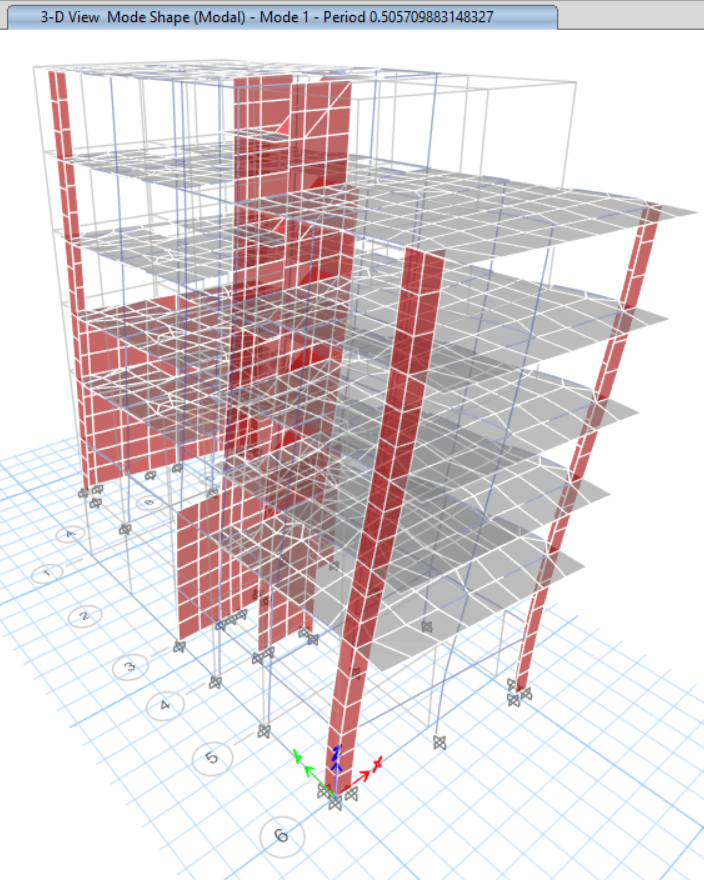
\includegraphics[height=10cm]{IMAGENES/11.PNG}
        \label{Imagen-Madrid}}
    \subfigure[2do Modo traslacional en X]{
        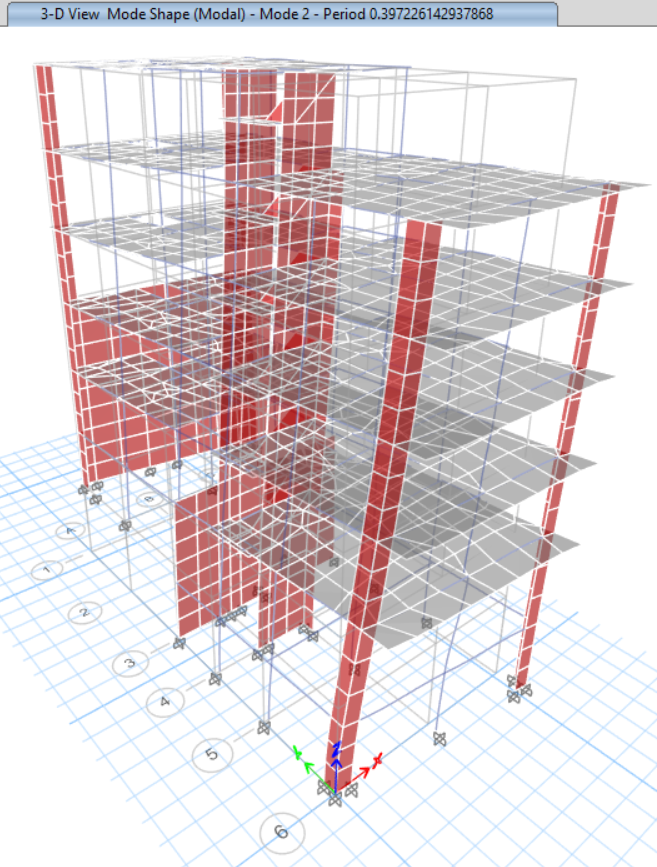
\includegraphics[height=10cm]{IMAGENES/13.PNG}
        \label{Imagen-Paris}}
    \subfigure[3er Modo torsional]{
        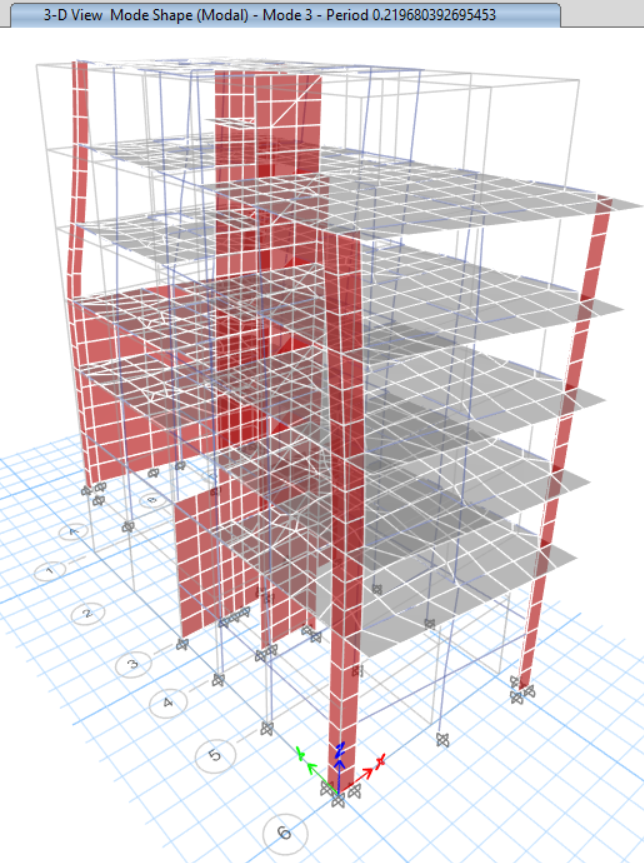
\includegraphics[height=10cm]{IMAGENES/14.PNG}
        \label{Imagen-Londres}}
    \caption{3 primeros modos de vibración}
    \label{Figura-Ciudades}
  \end{center}
\end{figure}
%\centering
%\fcolorbox{red}{yellow}{Caja de texto en amarillo con borde rojo}
%>{\centering\arraybackslash}m{2.5cm}
% Table generated by Excel2LaTeX from sheet 'Hoja5'
\newpage

\subsection{Análisis de irregularidades Art. 29 E-030}
\subsubsection{Irregularidad por discontinuidad del diafragma}
\begin{mybox2}{Tabla N°9}
\textit{La estructura se califica como irregular cuando los diafragmas 
tienen discontinuidades abruptas o variaciones importantes en 
rigidez, incluyendo aberturas mayores que 50\% del área bruta 
del diafragma.}\\
\textit{También  existe  irregularidad  cuando,  en  cualquiera de  los 
pisos y para cualquiera de las direcciones de análisis, se tiene 
alguna sección transversal del diafragma con un área neta 
resistente menor que 25\% del área de la sección transversal 
total de la misma dirección calculada con las dimensiones 
totales de la planta.}
\end{mybox2}

\begin{figure}[h!]
    \centering
    \caption{Irregularidad por discontinuidad del diafragma}
    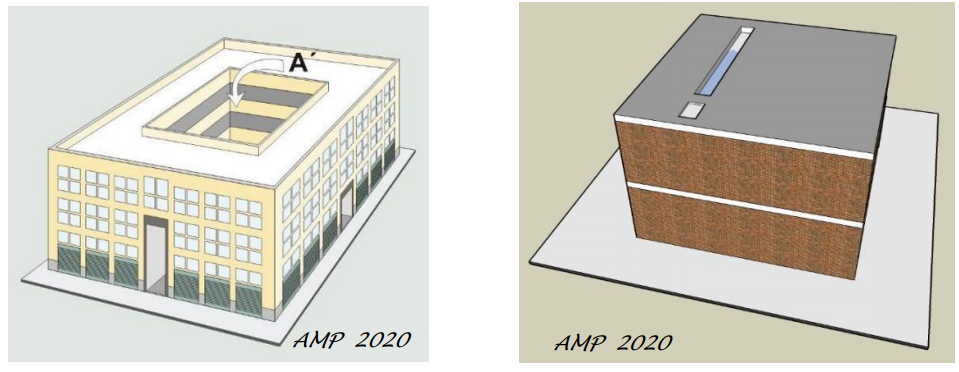
\includegraphics[scale=0.7]{IMAGENES/20.PNG}
    \caption*{\small Fuente: \it \cite{comen}}
    \label{fig:my_label}
    
\end{figure}

% Table generated by Excel2LaTeX from sheet '04) IRREG. DISCON.'
\begin{table}[h!]
  \centering
  \caption{Irregularidad por discontinuidad del diafragma (a)}
    \begin{tabular}{|ll|c|r}
\cline{1-3}    \multicolumn{2}{|l|}{Longitud del aligerado (L1)} & 7.51 & \multicolumn{1}{l}{m} \\
\cline{1-3}    \multicolumn{2}{|l|}{Espesor de losa superior del aligerado (e1)} & 0.05  & \multicolumn{1}{l}{m} \\
\cline{1-3}    \multicolumn{2}{|l|}{Area total del aligerado A1=L1.e1} & 0.38 & \multicolumn{1}{l}{m2} \\
\cline{1-3}    \multicolumn{2}{|l|}{Longitud de la losa maciza (L2)} & 2.55 & \multicolumn{1}{l}{m} \\
\cline{1-3}    \multicolumn{2}{|l|}{Espesor losa maciza (e2)} & 0.20  & \multicolumn{1}{l}{m} \\
\cline{1-3}    \multicolumn{2}{|l|}{Area de losa maciza A2=L2.e2} & 0.51 & \multicolumn{1}{l}{m2} \\
\cline{1-3}    \multicolumn{2}{|l|}{Ratio (A2/A1)} & 136.00 & \multicolumn{1}{l}{\%} \\
\cline{1-3}    \multicolumn{2}{|l|}{Limite <} & 25.00 & \multicolumn{1}{l}{\%} \\
\cline{1-3}    \multicolumn{2}{|l|}{Verificacion} & \textcolor[rgb]{ .267,  .447,  .769}{\textbf{Regular}} &  \\
\cline{1-3}    \end{tabular}%
  \label{tab:addlabel}%
\end{table}%

\begin{figure}[h!]
    \centering
    \caption{Aberturas en la planta del edificio}
    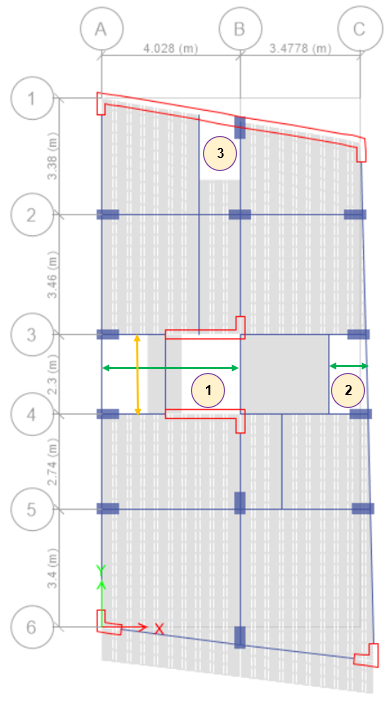
\includegraphics[scale=1]{IMAGENES/17.PNG}
    \label{fig:my_label}
\end{figure}

% Table generated by Excel2LaTeX from sheet '04) IRREG. DISCON.'
\begin{table}[h!]
  \centering
  \caption{Irregularidad por discontinuidad del diafragma (b)}
    \begin{tabular}{rr|l|c|r}
\cline{1-4}    \multicolumn{1}{|c|}{\textbf{Abertura}} & \multicolumn{1}{c|}{\textbf{Ancho (m)}} & \multicolumn{1}{c|}{\textbf{Largo (m)}} & \textbf{Area (m2)} &  \\
\cline{1-4}    \multicolumn{1}{|c|}{1} & \multicolumn{1}{c|}{4.028} & \multicolumn{1}{c|}{2.3} & 9.26  &  \\
\cline{1-4}    \multicolumn{1}{|c|}{2} & \multicolumn{1}{c|}{1.1} & \multicolumn{1}{c|}{2.3} & 2.53  &  \\
\cline{1-4}    \multicolumn{1}{|c|}{3} & \multicolumn{1}{c|}{1.2} & \multicolumn{1}{c|}{1.9} & 2.28  &  \\
\cline{1-4}          &       & Area total de aberturas & 14.07 &  \\
\cline{3-4}          & \multicolumn{1}{r}{} & \multicolumn{1}{r}{} & \multicolumn{1}{r}{} &  \\
\cline{3-4}          &       & Area total en planta  & 120.41 & \multicolumn{1}{l}{(m2)} \\
\cline{3-4}          &       & Ratio   & \textbf{11.689} & \multicolumn{1}{l}{\%} \\
\cline{3-4}          &       & Limite & \textbf{50.000} &  \\
\cline{3-4}          &       & Verificación & \textcolor[rgb]{ .267,  .447,  .769}{\textbf{Regular}} &  \\
\cline{3-4}    \end{tabular}%
  \label{tab:addlabel}%
\end{table}%

\subsubsection{Irregularidad por esquinas entrantes}

\begin{mybox2}{Tabla N°9 E-030}
\textit{La estructura se califica como irregular cuando tiene esquinas 
entrantes  cuyas  dimensiones  en  ambas  direcciones  son 
mayores que 20\% de la correspondiente dimensión total en 
planta}
\end{mybox2}

\begin{figure}[h!]
    \centering
    \caption{Irregularidad por esquinas entrantes}
    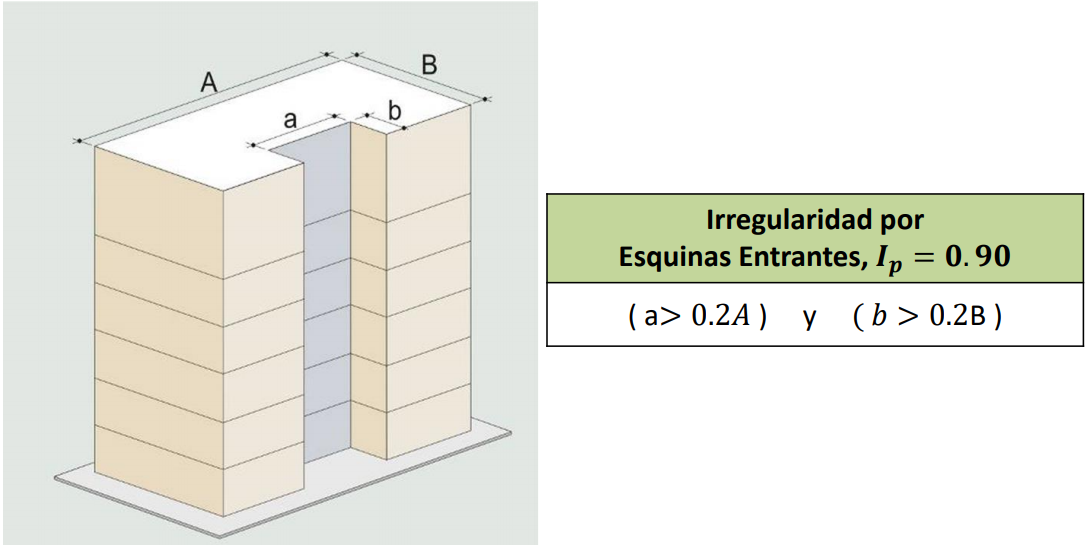
\includegraphics[scale=0.7]{IMAGENES/19.PNG}
    \caption*{\small Fuente: \it \cite{comen}}
    \label{fig:my_label}
\end{figure}

% Table generated by Excel2LaTeX from sheet '04) IRREG. DISCON.'
\begin{table}[h!]
  \centering
  \caption{Irregularidad por esquinas entrantes}
    \begin{tabular}{|ll|c|r}
\cline{1-3}    \multicolumn{2}{|l|}{Esquina entrante en X (a)} & 4.95  &  \\
\cline{1-3}    \multicolumn{2}{|l|}{Esquina entrante en Y (b)} & 2.30  &  \\
\cline{1-3}    \multicolumn{2}{|l|}{Dimensión total en X (A)} & 7.51  &  \\
\cline{1-3}    \multicolumn{2}{|l|}{Dimensión total en Y (B)} & 15.28 &  \\
\cline{1-3}    \multicolumn{2}{|l|}{a/A} & 66.00 & \multicolumn{1}{l}{\%} \\
\cline{1-3}    \multicolumn{2}{|l|}{b/B} & 15.05 & \multicolumn{1}{l}{\%} \\
\cline{1-3}    \multicolumn{2}{|l|}{Limite <} & 20.00 & \multicolumn{1}{l}{\%} \\
\cline{1-3}    \multicolumn{2}{|l|}{Verificación} & \textcolor[rgb]{ .267,  .447,  .769}{\textbf{Regular}} &  \\
\cline{1-3}    \end{tabular}%
  \label{tab:addlabel}%
\end{table}%


\subsection{Análisis Sísmico Dinámico Modal Espectral Art. 29 E-030}

El análisis dinámico modal espectral consiste calcular la respuesta para cada modo ingresando al espectro de pseudo-aceleraciones definido en , para posteriormente combinar los resultados según los criterios que se menciona en la norma E-030:

\subsubsection{Criterios de combinación}

\begin{mybox3}{Art. 26.3.1}
\textit{Mediante los criterios de combinación que se indican, se puede obtener la respuesta máxima elástica esperada (r) tanto para las fuerzas internas en los elementos componentes de la estructura, como para los parámetros globales 
del edificio como fuerza cortante en la base, cortantes de entrepiso, momentos 
de volteo, desplazamientos totales y relativos de entrepiso.}
\end{mybox3}

\begin{mybox3}{Art. 26.3.2}
\textit{La respuesta máxima elástica esperada (r) correspondiente al efecto conjunto 
de  los  diferentes  modos  de  vibración  empleados  (ri)  puede determinarse 
usando la combinación cuadrática completa de los valores calculados para 
cada modo.}
\end{mybox3}
\vspace{-0.8cm}
\begin{equation}
r=\sqrt{\sum \sum r_{i}\,\rho _{i}\,r_{i}}
\end{equation}
\myequations{Combinación cuadrática completa}

\begin{mybox3}{Art. 26.3.3}
\textit{Donde r representa las respuestas modales, desplazamientos o fuerzas, los coeficientes de correlación están dados por:}
\end{mybox3}

\vspace{-0.8cm}
\begin{equation}
\rho_{ij}=\frac{8\beta ^{2}\left ( 1+\lambda  \right )\lambda ^{3/2}}{\left ( 1-\lambda ^{2} \right )+4\beta ^{2}\lambda \left ( 1+\lambda  \right )^{2}}\,\,\,\,\,\,\,\,\,\,\,\lambda =\frac{\omega _{j}}{\omega _{i}}
\end{equation}
\myequations{Coeficientes de correlación}

\begin{flushleft}
Donde:\\
$\beta$: fracción del amortiguamiento crítico, que se puede suponer constante para todos los modos igual a 0,05.\\
$\omega _{j}$,$\omega _{i}$: son las frecuencias angulares de los modos i, j\\
\end{flushleft}

\subsection{Determinación de desplazamientos laterales Art. 28 E-030}
\begin{mybox3}{Art. 28.1}
\textit{Para  estructuras  regulares, los  desplazamientos  laterales  se  calculan 
multiplicando por 0,75 R los resultados obtenidos del análisis lineal y elástico con las solicitaciones sísmicas reducidas. Para estructuras irregulares, los 
desplazamientos laterales se calculan multiplicando por 0,85 R los resultados 
obtenidos del análisis lineal elástico.}
\end{mybox3}

\begin{figure}[h!]
    \centering
    \begin{tikzpicture}
    %draw[color=blue, help lines,dashed ] (0,0) grid (4.5,1.7);
    \begin{axis}
    [grid=both,
    grid style={line width=.1pt,dashed, draw=gray!10},
    major grid style={line width=.2pt,draw=gray!50},name=plot, xlabel={D (cm)},ylabel={h(m)},xmin=0,xmax=7,
    ymin=0,ymax=20,width=.6\textwidth,height=8cm,legend entries={X (R=6),Y(R=8)},legend pos=south east]%,xtick distance=.5%,ytick distance=.5]
    \addplot[OrangeRed,ultra thick,mark=o] table{DATOS/DX.txt};\label{xx}
    \addplot[MidnightBlue,ultra thick,mark=o] table{DATOS/DY.txt};\label{yy}
    \end{axis}

    \end{tikzpicture}
    \caption{Desplazamiento inelásticos}
    \label{fig:my_label}
\end{figure}

\subsection{Verificación de derivas máximas Art. 31 E-030}
% Table generated by Excel2LaTeX from sheet 'Hoja1'
\begin{table}[h!]
  \centering
  \caption{Derivas máximas}
    \begin{tabular}{|m{7cm}|c|}
    \hline
    \multicolumn{2}{|c|}{\multirow{2}[1]{*}{\textbf{LIMITES PARA LA DISTORSION DE ENTREPISO}}} \\
    \multicolumn{2}{|c|}{} \\
    \hline
    \textbf{Material predominante:} & $\Delta_{i}/h_{ei}$ \\
    \hline
    \rowcolor[rgb]{ .906,  .902,  .902} Concreto Armado & \textcolor[rgb]{ 1,  0,  0}{\textbf{0,007}} \\
    \hline
    Acero & 0,010 \\
    \hline
    Albañilería & 0,005 \\
    \hline
    Madera & 0,010 \\
    \hline
    Edificios de concreto armado con muros de ductilidad limitada & 0,005 \\
    \hline
    \end{tabular}%
    \caption*{\small Fuente: \it \cite{E-030}}
  \label{tab:addlabel}%
\end{table}%

\begin{figure}[h!]
    \centering
    \begin{tikzpicture}
    \begin{axis}
    [grid=both,
    grid style={line width=.1pt,dashed, draw=gray!10},
    major grid style={line width=.2pt,draw=gray!50},name=plot, xlabel={ $\Delta/h_{e}$},ylabel={h(m)},xmin=0,xmax=0.008,
    ymin=0,ymax=21,width=.6\textwidth,height=8cm,ytick distance=3,legend entries={X (R=6),Y(R=8)},legend pos=south east]
    \addplot[OrangeRed,ultra thick,mark=o] table{DATOS/DXX.txt};\label{xx}
    \addplot[MidnightBlue,ultra thick,mark=o] table{DATOS/DYY.txt};\label{yy}
    %\addplot[black,mark=triangle*] table{./espectro R=8.txt};\label{f}
    %\addplot[red,mark=o] table{./data/generator.txt};\label{g}
    %\addplot[blue] table{./data/simulated_total.txt};\label{s}
    %\addplot[green,dashed] table{./data/theoretical_total.txt};\label{t}
% Define two points for drawing an arrow to the "matched" point
    \node[] (C) at (axis cs: 0.007,20) {0.007};
    \node[] (B) at (axis cs: 0.007,3.5) {};
    \node[] (D) at (axis cs: 0.0035,20) {0.0035};
    \node[] (G) at (axis cs: 0.0035,0) {};
    \end{axis}
%\draw [dashed] (10,1) -- (10,11);
\draw[dashed,color=green,line width=1pt] (C)--(B);
\draw[dashed,color=orange,line width=1pt] (D)--(G);
%\node[anchor=west] (label) at (B) {matched};
    
    \end{tikzpicture}
    \caption{Derivas máximas de entrepiso}
    \label{der}
\end{figure}


\subsection{Verificación de Irregularidad torsional}
No es necesario verificar la irregularidad torsional en la dirección X dado que no se supera el 50\% de la deriva máxima permisible como se muestra en la figura \ref{der}.
\begin{figure}[h!]
    \centering
    \caption{Irregularidad torsional}
    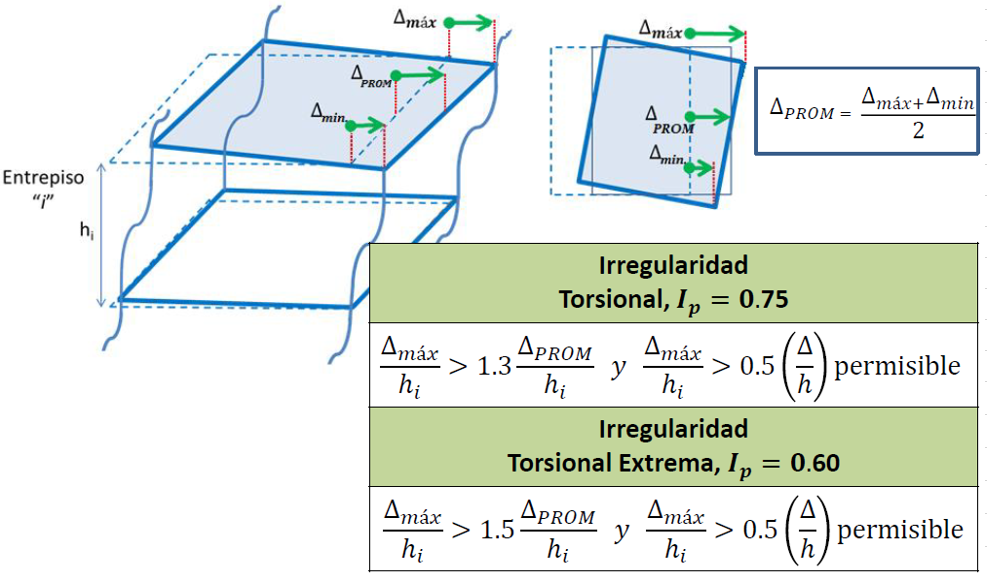
\includegraphics[scale=0.7]{IMAGENES/16.PNG}
    \caption*{\small Fuente: \it \cite{comen}}
    \label{fig:my_label}
\end{figure}

% Table generated by Excel2LaTeX from sheet 'Hoja2'
\begin{table}[h!]
  \centering
  \caption{Irregularidad torsional en la dirección Y}
    \begin{tabular}{|c|c|c|c|}
    \hline
    \multicolumn{1}{|c|}{\multirow{2}[4]{*}{\textbf{Piso}}} & \multicolumn{1}{p{5.39em}|}{\textbf{Max Drift}} & \multicolumn{1}{p{5.39em}|}{\textbf{Avg Drift}} & \multicolumn{1}{c|}{\multirow{2}[4]{*}{\textbf{Ratio}}} \\
\cline{2-3}          & \multicolumn{1}{c|}{\textbf{m}} & \multicolumn{1}{c|}{\textbf{m}} &  \\
    \hline
    6     & 0.004609 & 0.004136 & 1.114 \\
    \hline
    5     & 0.007212 & 0.006692 & 1.078 \\
    \hline
    4     & 0.010451 & 0.009752 & 1.072 \\
    \hline
    3     & 0.01278 & 0.011904 & 1.074 \\
    \hline
    2     & 0.014642 & 0.012545 & 1.167 \\
    \hline
    1     & 0.014251 & 0.012189 & 1.169 \\
    \hline
    \end{tabular}%
  \label{tab:addlabel}%
\end{table}%

El ratio no supera 1.3, por lo que el edificio en estudio no presenta irregularidad torsional.

\subsection{Verificación del sistema estructural}
Se verificara que efectivamente se tiene un sistema estructural de muros en la dirección X, en la dirección Y no se verificara dado que no existen muros estructurales. Como se muestra en la figura \ref{ver} el valor de cortante que absorben los muros es de 64 ton, y la cortante total es aproximadamente 70 ton (ver figura \ref{cor}) por lo que el porcentaje que toman los muros es mayor al 90\%.
\begin{figure}[h!]
    \centering
    \caption{Sistema estructural}
    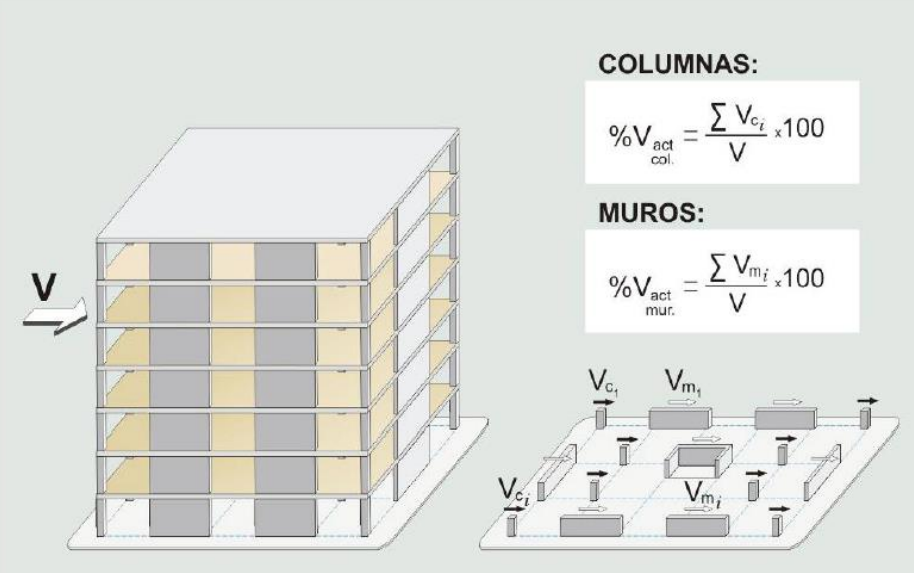
\includegraphics[scale=0.7]{IMAGENES/18.PNG}
    \caption*{\small Fuente: \it \cite{comen}}
    \label{fig:my_label}
\end{figure}
\newpage
\begin{figure}[h!]
    \centering
    \caption{Verificación del sistema estructural en X}
    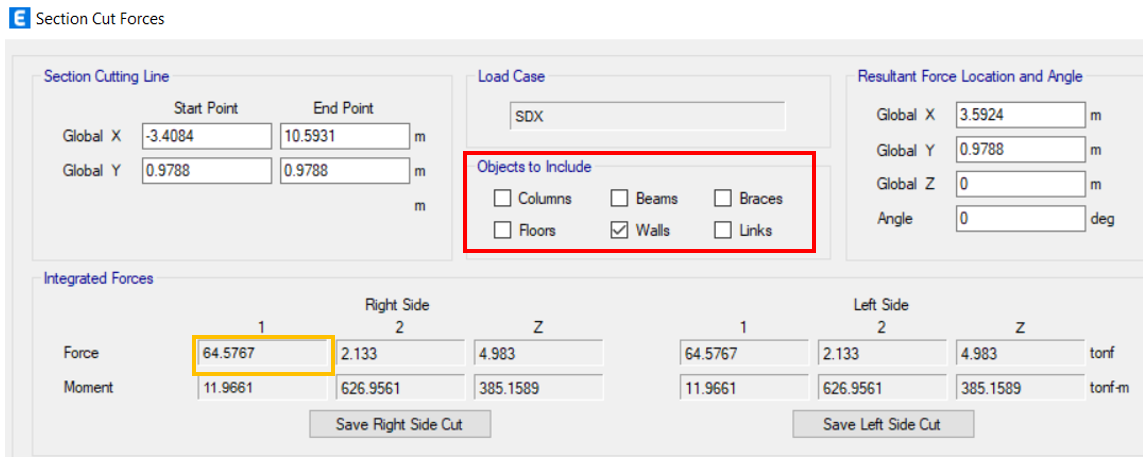
\includegraphics[scale=0.58]{IMAGENES/21.PNG}
    \label{ver}
\end{figure}

\subsection{Análisis estático o de fuerzas estáticas equivalentes Art. 25 E-030}
\subsubsection{Fuerza cortante en la base Art 25.2 E-030}

\begin{mybox3}{Art. 25.2.1}
\textit{La fuerza cortante total en la base de la estructura, correspondiente a la dirección considerada, se determina por la siguiente expresión:}
\end{mybox3}
%\vspace{-0.8cm}
\begin{equation}
V=\frac{Z\;\cdot U\cdot\;C\cdot\;S}{R}\;P\;\;\;\;\;\;\;\;\;\;\;\frac{C}{R}\geqslant 0,11
\end{equation}
\myequations{Cortante basal estática}
\noindent
Según el articulo 25.4.2 el periodo fundamental de vibración puede estimarse con la ecuación:

\begin{equation}
T=2\pi\cdot \displaystyle\sqrt{\frac{\left (\displaystyle\sum_{i=1}^{n} P_{i}\cdot d_{i}^{2}\right )}{g\cdot\left (\displaystyle\sum_{i=1}^{n}f_{i}\cdot d_{i}  \right ) }}
\end{equation}
\myequations{Periodo fundamental}
\noindent Donde:\\
$P_{i}$: es el peso sísmico en el nivel i.\\
$f_{i}$: es la fuerza lateral en el nivel i correspondiente a una distribución en altura semejante a la del primer modo en la dirección de análisis.\\
$d_{i}$: es el desplazamiento lateral del centro de masa del nivel  i en 
traslación pura (restringiendo los giros en planta) debido a las fuerzas 
$f_{i}$. Los desplazamientos se calculan suponiendo comportamiento lineal 
elástico de la estructura y, para el caso de estructuras de concreto 
armado y de albañilería, considerando las secciones sin fisurar.\\
\\
Lo anterior equivale a calcular los modos de vibrar en el modelo matemático restringiendo el grado de libertad de rotación.

\begin{figure}[h!]
    \centering
    \subfigure[X]{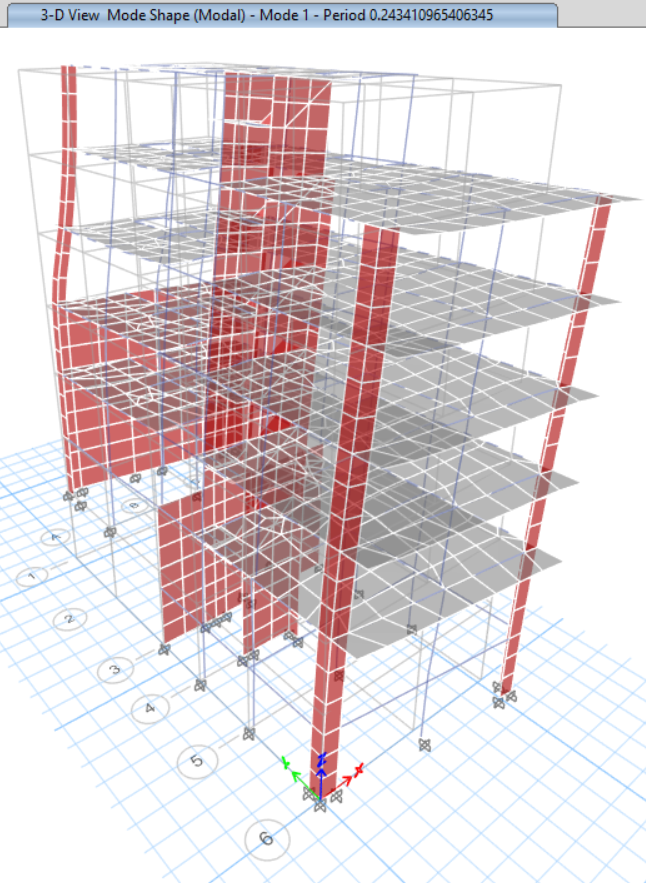
\includegraphics[height=70mm]{IMAGENES/TX.PNG}}\hspace{10mm}
    \subfigure[Y]{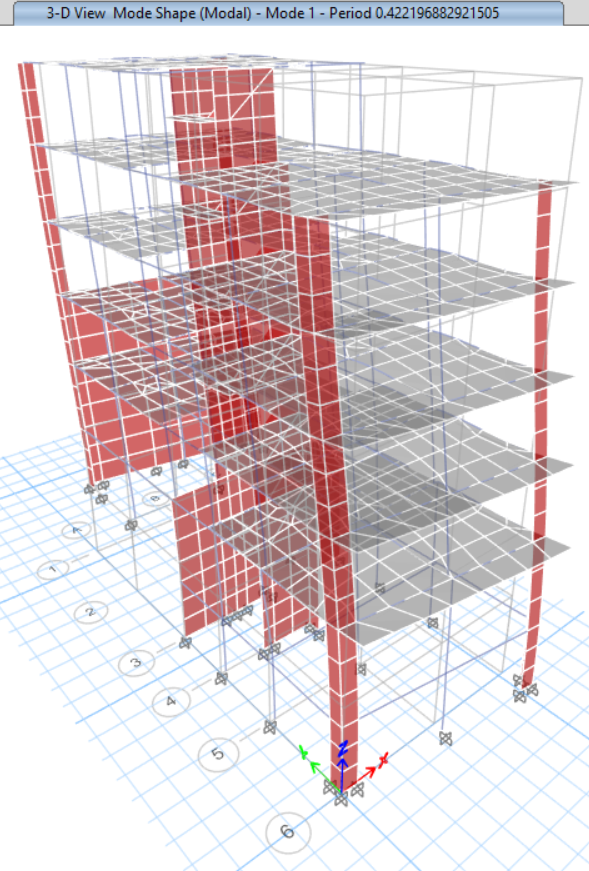
\includegraphics[height=70mm]{IMAGENES/TY.PNG}}
    \caption{Periodos fundamentales en traslación pura}
    \label{3}
\end{figure}
\newpage
% Table generated by Excel2LaTeX from sheet 'ASE'
\begin{table}[h!]
  \centering
  \caption{Análisis Sísmico Estático}
      {
\extrarowheight = 0ex
\renewcommand{\arraystretch}{1.2}
    \begin{tabular}{>{\arraybackslash}m{7cm}|>{\centering\arraybackslash}m{2.5cm}|>{\centering\arraybackslash}m{2cm}|>{\centering\arraybackslash}m{2cm}|}
\cline{2-4}          & \multicolumn{3}{c|}{\textit{\textbf{PARAMETROS SISMICOS}}} \\
\cline{2-4}          &       & \textbf{X} & \textbf{Y} \\
\cline{2-4}    \textit{Factor de Zona (Tabla N°1)} & \textbf{Z} & \multicolumn{2}{c|}{0.25} \\
\cline{2-4}    \textit{Factor de Uso (Tabla N°5)} & \textbf{U} & \multicolumn{2}{c|}{1.00} \\
\cline{2-4}    \textit{Periodos en traslación pura obtenidos del ETABS (Art. 25.4.2)} & \textbf{T} & 0.24  & 0.42 \\
\cline{2-4}    \textit{Factor de Amplificación (Art. 14)} & \textbf{C} & 2.50  & 2.50 \\
\cline{2-4}    \textit{Factor de Suelo (Tabla N°3)} & \textbf{S} & \multicolumn{2}{c|}{1.40} \\
\cline{2-4}    \textit{Coef. Básico de Reducción (Tabla N°7)} & \textbf{Ro} & 6.00  & 8.00 \\
\cline{2-4}    \textit{Irregularidad en altura (Tabla N°8)} & \textbf{Ia} & 1.00  & 1.00 \\
\cline{2-4}    \textit{Irregularidad en planta (Tabla N°9)} & \textbf{Ip} & 1.00  & 1.00 \\
\cline{2-4}    \textit{Coef. de Reducción (Articulo 22)} & \textbf{R} & 6.00  & 8.00 \\
\cline{2-4}    \textit{Verificación Art. 28.2.2} & \textbf{C/R$>$0.11} & 0.42  & 0.42 \\
\cline{2-4}    \textit{Carga Muerta (CM)} & \textbf{PD} & \multicolumn{2}{c|}{748.42} \\
\cline{2-4}    \textit{Carga Viva (CV)} & \textbf{PL} & \multicolumn{2}{c|}{108.84} \\
\cline{2-4}    \textit{Peso Sísmico (ETABS)} & \textbf{Ps (Ton)} & \multicolumn{2}{c|}{775.63} \\
\cline{2-4}    \textit{Coeficientes} & \textbf{ZUCS/R} & 0.15  & 0.11 \\
\cline{2-4}    \textit{Cortante Estática (Art. 28.2)} & \textbf{V (Ton)} & \cellcolor[rgb]{ 1,  .949,  .8}\textcolor[rgb]{ 1,  0,  0}{\textbf{113.11}} & \cellcolor[rgb]{ 1,  .949,  .8}\textcolor[rgb]{ 1,  0,  0}{\textbf{84.83}} \\
\cline{2-4}    Coeficiente k (Art. 28.3.2) & \textbf{k} & 1.00  & 1.00 \\
\cline{2-4}    \end{tabular}%
}
  \label{tab:addlabel}%
\end{table}%

\subsection{Fuerza cortante mínima Art. 26.4 E-030}
\begin{mybox2}{Art. 26.4.1}
\textit{Para cada una de las direcciones consideradas en el análisis, la fuerza cortante en el primer entrepiso del edificio no puede ser menor que el 80\% del valor calculado según el artículo 25 para estructuras regulares, ni menor que el 90\% para estructuras irregulares..}
\end{mybox2}

%\newmdenv[innerlinewidth=0.5pt, roundcorner=4pt,linecolor=mycolor,innerleftmargin=6pt, innerrightmargin=6pt,innertopmargin=6pt,innerbottommargin=6pt]{myboxx}

\begin{mybox2}{Art. 26.4.2 E-030}
\textit{Si fuera necesario incrementar el cortante para cumplir los mínimos señalados,  se escalan proporcionalmente todos los otros resultados obtenidos, excepto los  desplazamientos.}
\end{mybox2}
\newpage
\begin{figure}[ht!]
    \centering
    \begin{tikzpicture}
    %draw[color=blue, help lines,dashed ] (0,0) grid (4.5,1.7);
    \begin{axis}
    [grid=both,
    grid style={line width=.1pt,dashed, draw=gray!10},
    major grid style={line width=.2pt,draw=gray!50},name=plot, xlabel={V (ton)},ylabel={h(m)},xmin=0,xmax=70,
    ymin=0,ymax=20,width=.8\textwidth,height=10cm,legend entries={X (R=6),Y(R=8)},legend pos=north east]%,xtick distance=.5%,ytick distance=.5]
    \addplot[OrangeRed,ultra thick] table{DATOS/VX.txt};\label{xx}
    \addplot[MidnightBlue,ultra thick] table{DATOS/VY.txt};\label{yy}
    \end{axis}
    \end{tikzpicture}
    \caption{Cortantes de entrepiso del AME}
    \label{cor}
\end{figure}
%\vspace{-2cm}
% Table generated by Excel2LaTeX from sheet 'ESCALAM'
\begin{table}[h!]
  \centering
  \caption{Escalamiento de la cortante dinámica}
        {
\extrarowheight = 0ex
\renewcommand{\arraystretch}{1.2}
    \begin{tabular}{|l|c|>{\centering\arraybackslash}m{2cm}|>{\centering\arraybackslash}m{2cm}|}
\cline{3-4}    \multicolumn{1}{r}{} &       & \textbf{X} & \textbf{Y} \\
    \hline
    \textit{Cortante dinámica} & \textbf{V dina (Ton)} & 69.85 & 66.86 \\
    \hline
    \textit{Cortante estático} & \textbf{V est (Ton)} & 113.11 & 84.83 \\
    \hline
    \textit{Porcentaje} & \textbf{\%} & 61.75 & 78.81 \\
    \hline
    \textit{Porcentaje mínimo} & \textbf{V min \%} & 80.00 & 80.00 \\
    \hline
    \textit{Factor de escala} & \textbf{F.E.} & 1.30  & 1.02 \\
    \hline
    \textit{Cortante dinámica escalada} & \textbf{V dina esc.} & 90.49 & 67.87 \\
    \hline
    \end{tabular}%
    }
  \label{tab:addlabel}%
\end{table}%


\subsection{Separación entre edificios Art. 30 E-030}
\begin{mybox2}{Art. 30.1}
\textit{Toda estructura está separada de las estructuras vecinas, desde el nivel del terreno natural, una distancia mínima s para evitar el contacto durante un movimiento sísmico.}
\end{mybox2}

\begin{mybox2}{Art. 30.2}
\textit{Esta distancia no es menor que los 2/3 de la suma de los desplazamientos máximos de los edificios adyacentes ni menor que:}
\end{mybox2}
%\vspace{-0.8cm}
\begin{equation}
s=0.006\;h\geq0.03\;m
\end{equation}
\myequations{Separación mínima entre edificios}
\noindent Donde h es la altura medida desde el nivel del terreno natural hasta el nivel considerado para evaluar s.

\begin{mybox2}{Art. 30.2}
\textit{El edificio se retira de los límites de propiedad adyacentes a otros lotes edificables,  o  con  edificaciones,  distancias  no  menores  que  2/3  del desplazamiento máximo calculado según el artículo 28 ni menores que s/2 si la edificación existente cuenta con una junta sísmica reglamentaria.}
\end{mybox2}

\begin{figure}[h!]
    \centering
    \caption{Separación entre edificios}
    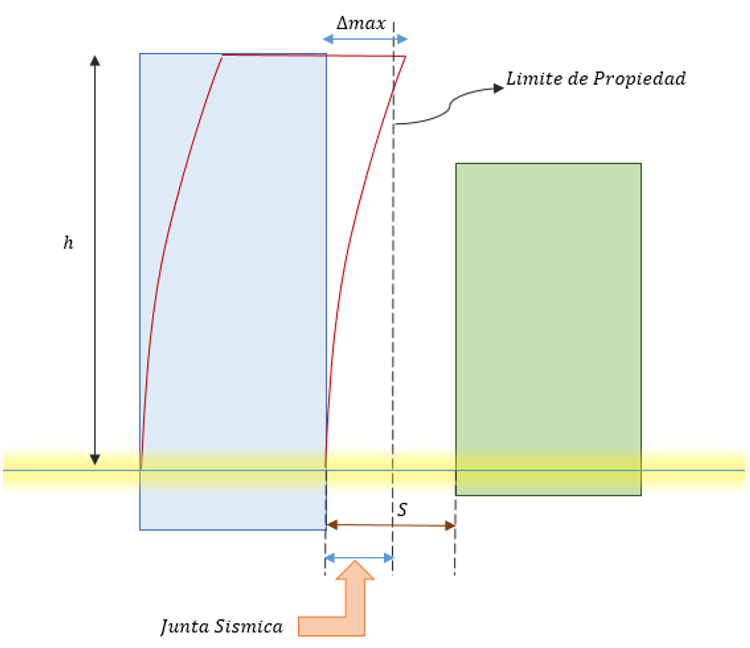
\includegraphics[scale=0.67]{IMAGENES/23.PNG}
    \label{ver}
\end{figure}
\newpage
% Table generated by Excel2LaTeX from sheet 'Hoja1'
\begin{table}[h!]
  \centering
  \caption{Calculo de la junta sísmica}
  \vspace{0.5cm}
      {
\extrarowheight = -0.3ex
\renewcommand{\arraystretch}{1.35}
    \begin{tabular}{l|c|c|l}
\cline{2-3}    \textit{Altura del edificio } & \textbf{h} & 1410.00 & cm \\
\cline{2-3}    \textit{Separación mínima entre edificios } & \textbf{s=0.006h} & 8.46  & $>$3cm \\
\cline{2-3}    \textit{Separación mínima del limite de propiedad} & \textbf{s/2} & 4.23  & cm \\
\cline{2-3}    \textit{Desplazamiento máximo en X } & \textbf{$\Delta _{x}$} & 4.81  & cm \\
\cline{2-3}    \textit{Desplazamiento máximo en Y } & \textbf{$\Delta _{y}$} & 6.07  & cm \\
\cline{2-3}    \textit{Separación del limite de propiedad X} & \textbf{2/3$\Delta _{x}$} & 3.21  & cm \\
\cline{2-3}    \textit{Separación del limite de propiedad Y} & \textbf{2/3$\Delta _{y}$} & 4.05  & cm \\
\cline{2-3}    \end{tabular}%
}
  \label{jun}%
\end{table}%

\noindent Según lo calculado en la tabla \ref{jun}  el edificio tendrá que ser separado del limite de propiedad 4.50cm como mínimo en ambas direcciones, en el caso que no exista junta reglamentaria el edificio actual se separa del edificio existente el valor de s/2 que le corresponde más el valor s/2 de la estructura vecina.
\section{Método de diseño}
Según el capítulo 9 de la norma E-060 la resistencia de diseño de todos los elementos debe ser por lo menos la resistencia requerida según:
\begin{equation}
   \phi R_{n}\geqslant R_{u} 
\end{equation}
\myequations{Requisito de resistencia según E-060}
\vspace{-1.4cm}
\section{Combinaciones de diseño}
Según el capitulo 9 de la \cite{E-060} las combinaciones de diseño serán:
    \begin{align}
       &U=1.4\;CM+1.7\;CV\myequations{Combinaciones de carga gravitacional} \\
        &U=1.25\left ( CM+CV \right )\pm CS\myequations{Combinaciones con carga sísmica 1}\\
        &U=0.9\;CM+CV \pm CS \myequations{Combinaciones con carga sísmica 2}        
    \end{align}

\newpage
\noindent
Donde:\\
$CM$: Carga Muerta\\
$CV$: Carga viva\\
$CS$: Carga de sismo, según la \cite{E-030} en el artículo 21.1 el análisis se puede realizar considerando que el total de la fuerza sísmica actúa independiente en cada dirección ortogonal, por lo que se tienen 5 combinaciones independientes considerando el sismo en cada dirección.
\section{Diseño de elementos estructurales}
\subsection{Diseño de vigas}
\subsubsection{Factores de minoración}
% Table generated by Excel2LaTeX from sheet 'Hoja1'
\begin{table}[ht!]
  \centering
  \caption{Factores de minoración para el diseño de vigas}
        {
\extrarowheight = 0ex
\renewcommand{\arraystretch}{1.15}
    \begin{tabular}{|>{\centering\arraybackslash}m{2.8cm}|>{\centering\arraybackslash}m{3.8cm}|>{\centering\arraybackslash}m{3.8cm}|}
    \hline
    \textbf{Articulo de E-060} & \textbf{Solicitación} & \textbf{Factor de minoración} \\
    \hline
    9.2.3.1   & Flexión & $\phi_{f}$=0.90 \\
    \hline
    9.3.2.3   & Corte y torsión & $\phi_{c}$=0.85 \\
    \hline
    \end{tabular}%
    }
    \caption*{\small Fuente: \it \cite{E-060}}
  \label{tab:addlabel}%
\end{table}%
\vspace{-0.8cm}
\subsubsection{Diseño a flexión}
\begin{figure}[h!]
    \centering
    \caption{Análisis de una viga simplemente armada}
    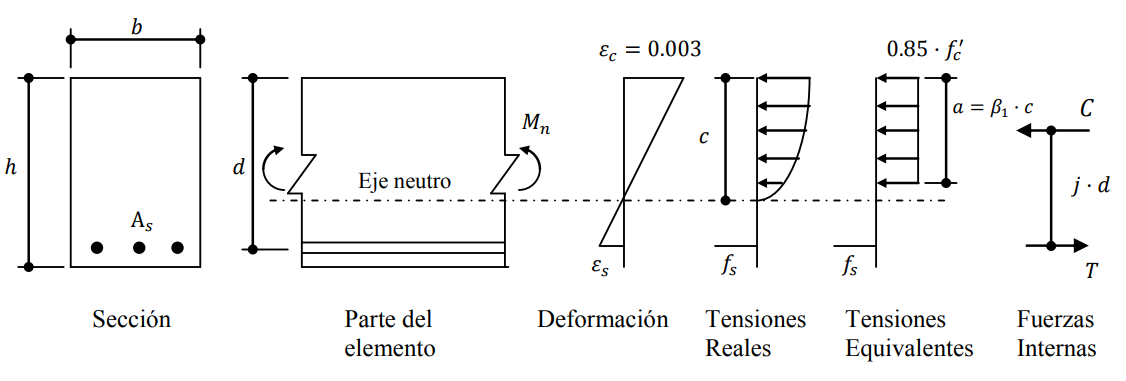
\includegraphics[scale=0.67]{IMAGENES/d9.PNG}
    \caption*{\small Fuente: \it \cite{cordova2015}}
    \label{vig}
\end{figure}
\begin{theo}[Art. 10.2.7.1 y 10.2.7.3 E-060 :]{thm:ca1}
Un  esfuerzo  en  el  concreto  de  0,85  f’c uniformemente  distribuido  en  una  zona  de compresión equivalente, limitada por los bordes de la sección transversal del elemento y por una línea recta paralela al eje neutro, a una distancia a = $\beta$c de la fibra de deformación unitaria máxima en compresión.\\
Para f’c entre 17 y 28 MPa, el factor $\beta$1 se debe tomar como 0,85.   Para f’c mayor o igual a 56 MPa,  $\beta$1 se debe tomar como 0,65.  Para f’c entre 28 y 56 MPa se debe interpolar linealmente entre 0,85 y 0,65.
\end{theo}
\noindent
%\vspace{-1cm}
Considerando que el acero de refuerzo alcanza la fluencia y los esfuerzos del concreto se representan mediante el bloque de compresión equivalente según la figura \ref{vig} y la \cite{E-060}:
\begin{flalign}
&\textup{Tracción en el acero de refuerzo:}&T&=A_{s}\cdot f_{y}&\\
&\textup{Compresión en el concreto:}&C&=0.85\cdot f_{c}^{'}\cdot a\cdot b&\\
&\textup{Brazo del par de fuerzas:}&j&=d-\frac{a}{2}&\\
&\textup{Momento resistente:}&\phi\cdot M_{n}&=\phi\cdot A_{s}\cdot f_{y}\left ( d-\frac{a}{2} \right )\label{15}&
\end{flalign}
\noindent
Haciendo uso de la ecuación de equilibrio $T&=C$ se puede llegar a la ecuación  (\ref{16}), y combinándola con (\ref{15}) haciendo uso de $M_{u}=\phi M_{n}$ se puede llegar a la expresión (\ref{ace}) para calcular el acero de refuerzo en una viga ignorando el refuerzo en compresión para un momento ultimo dado $M_{u}$.
\begin{gather}
%M_{u}&=\phi\cdot A_{s}\cdot f_{y}\left ( d-\frac{a}{2} \right )\label{15}&\\
a=\frac{A_{s}\cdot f_{y}}{0.85\cdot f_{c}^{'}\cdot b}\label{16}\\
A_{s}=\frac{0.85\;f_{c}^{'}\;b\;d}{f_{y}}\left ( 1-\sqrt{1-\frac{2\;M_{u}}{\phi\;0.85\;f_{c}^{'}\;b\;d^{2} }} \right )
\label{ace}
\end{gather}
\newpage
\noindent En la figura \ref{vigm} se muestra que la viga del eje 6 es la que presenta mayor solicitación de momento para la condición de envolvente de las combinación de diseño con las fuerzas sísmicas escaladas. A continuación se muestra el diseño del elemento mencionado.
\begin{figure}[h!]
    \centering
    \caption{Viga con mayor solicitación}
    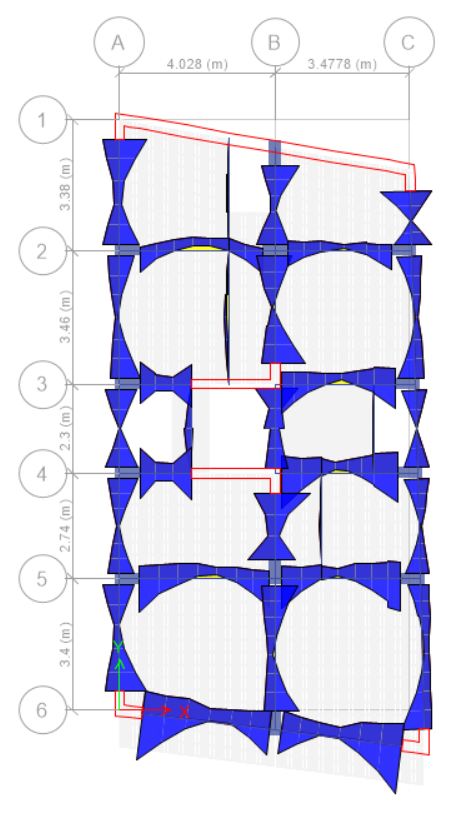
\includegraphics[scale=0.8]{IMAGENES/d10.PNG}
    %\caption*{\small Fuente: \it \cite{cordova2015}}
    \label{vigm}
\end{figure}

\newpage
\begin{figure}[h!]
    \centering
    \begin{tikzpicture}
        \tikzset{
        hatch distance/.store in=\hatchdistance,
        hatch distance=10pt,
        hatch thickness/.store in=\hatchthickness,
        hatch thickness=2pt
    }

    \makeatletter
    \pgfdeclarepatternformonly[\hatchdistance,\hatchthickness]{flexible hatch}
    {\pgfqpoint{0pt}{0pt}}
    {\pgfqpoint{\hatchdistance}{\hatchdistance}}
    {\pgfpoint{\hatchdistance-1pt}{\hatchdistance-1pt}}%
    {
        \pgfsetcolor{\tikz@pattern@color}
        \pgfsetlinewidth{\hatchthickness}
        \pgfpathmoveto{\pgfqpoint{0pt}{0pt}}
        \pgfpathlineto{\pgfqpoint{0pt}{\hatchdistance}}
        %\pgfpathlineto{\pgfqpoint{\hatchdistance}{\hatchdistance}}
        \pgfusepath{stroke}
    }
    \begin{axis}
    [grid=both,
    grid style={line width=.1pt,dashed, draw=gray!10},
    major grid style={line width=.2pt,draw=gray!50},name=plot, xlabel={$x$ (m)},ylabel={$M_{u}$ (ton.m)},xmin=0.15,xmax=3.3,
    ymin=-6,ymax=10,width=.85\textwidth,height=8cm,xtick distance=0.4,ytick distance=3]
    \addplot[name path = A,OrangeRed,ultra thick]
    table{DATOS/env.txt};\label{xx}
    \addplot[name path = B,MidnightBlue,ultra thick] table{DATOS/env2.txt};\label{yy}
    %\addplot[MidnightBlue,ultra thick,mark=o] table{DATOS/DYY.txt};\label{yy}
    %\addplot[black,mark=triangle*] table{./espectro R=8.txt};\label{f}
    %\addplot[red,mark=o] table{./data/generator.txt};\label{g}
    %\addplot[blue] table{./data/simulated_total.txt};\label{s}
    %\addplot[green,dashed] table{./data/theoretical_total.txt};\label{t}
   % \tikzfillbetween[of=A and B]{pattern=flexible hatch};
    \addplot[pattern=flexible hatch,
        hatch distance=7pt,hatch thickness=0.5pt,
        pattern color=cyan] fill between [of=A and B];
    \end{axis}
    \end{tikzpicture}
    \caption{Diagrama de momento flector viga EJE 6 tramo B-C (Envolvente)}
    \label{der}
\end{figure}
\noindent 

Geometría de la viga:
\FPset\h{50} 
\FPset\bv{30} 
\FPset\ln{3.15} 
\FPeval{\defe}{round(\h-6,0)}
\begin{itemize}
  \item Ancho: $b=30 \mathrm{~cm}$

  \item Peralte: $h=\h \mathrm{~cm}$

  \item Peralte efectivo: $d=h-6 \mathrm{~cm}\footnote{\cite{pasino2011} recomienda estimar el peralte efectivo como $d=h-6$ y $d=h-9$ para 1 y 2 capas de acero respectivamente}=\h-6=\defe \mathrm{~cm}$ 

  \item Luz libre: $l_{n}=\ln \mathrm{~m}$
  
\end{itemize}

Datos de los materiales:

Concreto:

\begin{itemize}
  \item Resistencia a la compresión: $\displaystyle f_{c}^{\prime}=210 \;\frac{\mathrm{kg}}{\mathrm{cm}^{2}}$

  \item Deformación unitaria del concreto: $\varepsilon_{c}=0,003$

  \item Densidad del concreto: $\displaystyle\gamma_{c}=2,40\;\frac{\mathrm{ ton }}{\mathrm{m}^{3}}$

\end{itemize}
\newpage
Acero de refuerzo:

\begin{itemize}
  \item Esfuerzo de fluencia: $\displaystyle f_{y}=4200\; \frac{\mathrm{kg}}{\mathrm{cm}^{2}}$

  \item Módulo de elasticidad: $\displaystyle E_{\mathrm{s}}=2 \cdot 10^{6} \;\frac{\mathrm{kg}}{\mathrm{cm}^{2}}$

  \item Deformación de fluencia: $\displaystyle \varepsilon_{s}=\frac{f_{y}}{E_{s}}=\frac{4200}{2 \cdot 10^{6}}=0,0021$

\end{itemize}
\noindent Aplicando la ecuación \ref{ace} se obtiene que se requiere para el extremo izquierdo $3.17\;{\mathrm{cm}^{2}}$ y $2.54\;{\mathrm{cm}^{2}}$ superior e inferior respectivamente y para el extremo derecho $6.19\;{\mathrm{cm}^{2}}$ y $3.17\;{\mathrm{cm}^{2}}$.\\
Por lo que se coloca $2 \phi 5 / 8"=3.96 \mathrm{~cm}^{2}$ como acero corrido superior e inferior y en el extremo superior derecho se coloca como bastón $2 \phi 5 / 8$" haciendo un total de $4 \phi 5 / 8"=7.92 \mathrm{~cm}^{2}$.\\
\textit{Verificación del espaciamiento entre barras}\\
Según el articulo 7.6.2 y 3.3.2 la distancia libre entre barras paralelas de una capa debe ser el mayor de:
\begin{enumerate}
\item[] (a): $d_{b}$ Diámetro de la varilla longitudinal
\item[] (b): $25 \mathrm{~mm}$
\item[] (c): $4/3$ del tamaño máximo del agregado
\end{enumerate}

\begin{figure}[h!]
    \centering
    \caption{Requisitos de colocación del refuerzo}
    \subfigure[Espaciamiento mínimo entre barras]{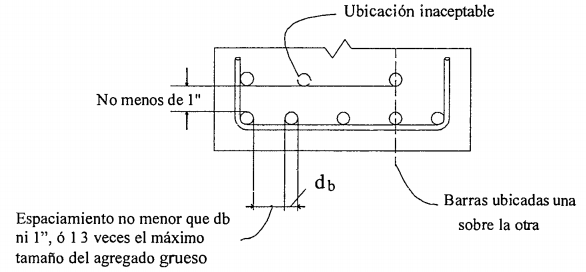
\includegraphics[height=45mm]{IMAGENES/sep.PNG}}\hspace{5mm}
    \subfigure[Recubrimiento]{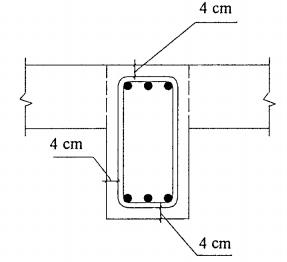
\includegraphics[height=45mm]{IMAGENES/rec.PNG}}
    \caption*{\small Fuente: \it \cite{pasino2011}}
    \label{3}
\end{figure}
Según el articulo 7.7.1 el recubrimiento mínimo para vigas de concreto construidos en sitio sin exposición a la intemperie ni al contacto con el suelo es de 4cm.

La separación entre barras donde existen $4 \phi 5 / 8"$ considerando estribos de 3/8" de diámetro ($d_{e}$) el peralte efectivo sera::
\FPset\rec{4}
\FPset\numvar{4}
\FPeval{\estcm}{round(3*2.54/8,2)}
\FPeval{\vacm}{round(5*2.54/8,2)}
\FPeval{\smin}{round((\bv-2*\rec-2*\estcm-\numvar*\vacm)/(\numvar-1),2)}
\begin{flalign}
s_{var}&=\frac{b-2\cdot r_{e}-2\cdot d_{e}-n_{v}\cdot d_{b}}{n_{v}-1}\\
s_{var}&=\frac{\bv-2\cdot \rec-2\cdot\estcm-\numvar\cdot \vacm}{\numvar-1}=\smin\mathrm{~cm}\notag
\end{flalign}
\textit{Peralte efectivo}
\FPeval{\deft}{round(\h-\rec-\estcm-\vacm/2,2)}
\begin{flalign}
d_{efe}&=h-r_{e}-d_{e}-d_{b}/2\\
d_{efe}&=\h-\rec-\estcm-\vacm/2=\deft\mathrm{~cm}\notag
\end{flalign}
La altura del bloque en compresión y el momento resistente del acero corrido sera:
\FPset\ascor{3.96}
\FPset\asder{7.92}
\FPset\fc{210}
\FPset\fy{4200}
\FPeval{\acor}{round((\fy*\ascor)/(0.85*\fc*\bv),2)}
\FPeval{\mncor}{round((0.9*\fy*\ascor)*(\defe-\acor/2)/100000,2)}
\begin{align*}
a&=\frac{A_{s}\cdot f_{y}}{0.85\cdot f_{c}^{'}\cdot b}\\
a&=\frac{\ascor\cdot \fy}{0.85\cdot\fc\cdot\bv}=\acor\;\mathrm{~cm}\\
\phi M_{n}&=\phi\cdot A_{s}\cdot f_{y}\left ( d-\frac{a}{2} \right )\\
\phi M_{n,1}&=0.9\cdot \ascor \cdot \fy\left ( \defe-\frac{\acor}{2} \right )=\mncor\;\mathrm{~ton.m} 
\end{align*}
\FPeval{\ader}{round((\fy*\asder)/(0.85*\fc*\bv),2)}
\FPeval{\mnder}{round((0.9*\fy*\asder)*(\defe-\ader/2)/100000,2)}
Similarmente en el extremo superior derecho:
\begin{align*}
%a&=\frac{A_{s}\cdot f_{y}}{0.85\cdot f_{c}^{'}\cdot b}\\
a&=\frac{\asder\cdot \fy}{0.85\cdot\fc\cdot\bv}=\ader\;\mathrm{~cm}\\
%\phi M_{n}&=\phi\cdot A_{s}\cdot f_{y}\left ( d-\frac{a}{2} \right )\\
\phi M_{n,2}&=0.9\cdot \asder \cdot \fy\left ( \defe-\frac{\ader}{2} \right )=\mnder\;\mathrm{~ton.m} 
\end{align*}
\newpage

\subsubsection{Desarrollo del refuerzo para flexión Art. 12.10}
%\newpage
\begin{theo}[Art. 12.10.3 :]{thm:ca1}
El refuerzo se debe extender, más allá del punto en el que ya no es necesario para resistir flexión, una distancia igual a d ó 12 db, la que sea mayor, excepto en los apoyos de vigas simplemente apoyadas y en el extremo libre de los voladizos.
\end{theo}
\noindent
Donde:\\
$d_{b}$ : Diámetro de la varilla\\
$d$ : Peralte efectivo\\

\begin{figure}[h!]
    \centering
    \caption{Punto teórico de corte}
    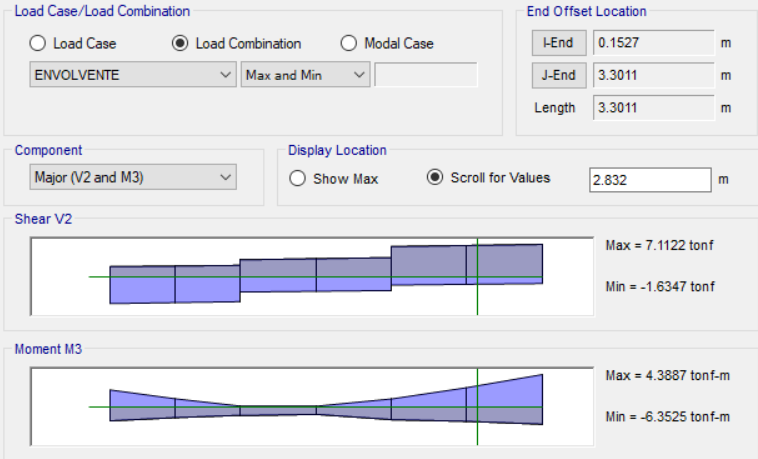
\includegraphics[scale=0.7]{IMAGENES/pcor.PNG}
    %\caption*{\small Fuente: \it \cite{cordova2015}}
    \label{vigcor}
\end{figure}

\begin{figure}[h!]
    \centering
    \caption{Corte de acero}
    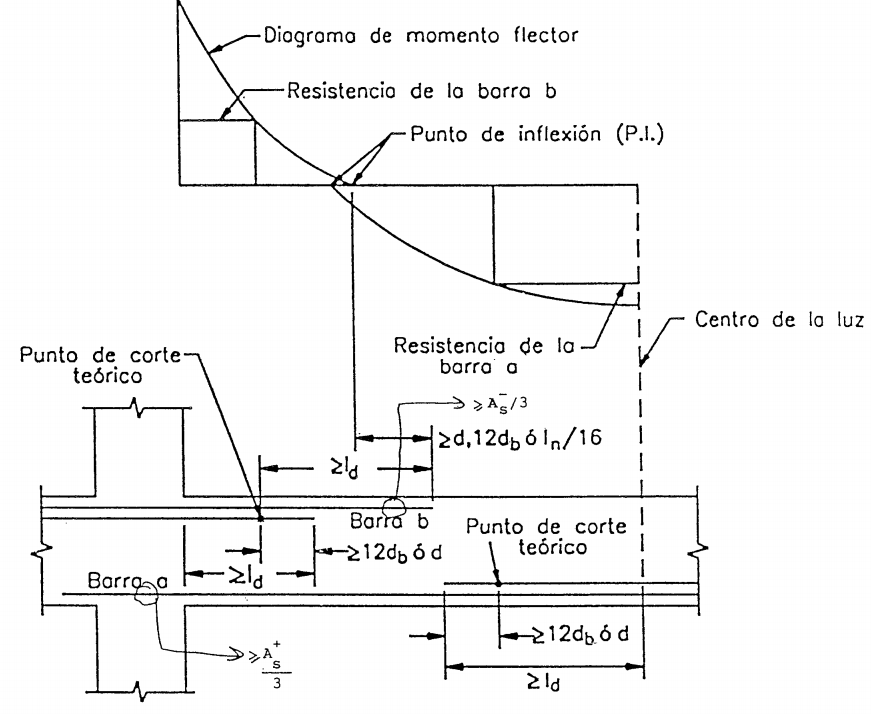
\includegraphics[scale=0.6]{IMAGENES/corte.PNG}
    \caption*{\small Fuente: \it \cite{pasino2011}}
    \label{vigm}
\end{figure}

\noindent La mayor dimensión entre d y 12 db resulta d=44 cm. Como se aprecia en la figura \ref{vigcor} la longitud teórica de corte sera: 3.3011m - 2.832m=0.469m, la longitud del bastón sera: 46.9cm+44cm $\approx$ 100cm.
\newpage
\begin{theo}[Art. 12.1 :]{thm:ca1}
La tracción o compresión calculada en el refuerzo en cada sección de los elementos de concreto estructural, debe ser desarrollada hacia cada lado de dicha sección mediante una longitud embebida en el concreto (longitud de anclaje), gancho, dispositivo mecánico o una combinación de ellos. Los ganchos no se deben emplear para el anclaje de barras en compresión.
\end{theo}
\noindent
Según la tabla 12.1 de la \cite{E-060} la longitud de desarrollo se calcula con la ecuación \ref{ld}
\begin{align}
l_{d}=\left(\frac{f_{y} \cdot \psi_{t} \cdot \psi_{e} \cdot \lambda}{8,2 \cdot \sqrt{f_{c}^{\prime}}}\right) d_{b}
\label{ld}
\end{align}
\noindent
Donde:\\
$\psi_{t}=1,3$ Para varillas superiores\\
$\psi_{e}=1,0$ Para varillas sin tratamiento superficial\\
$\lambda=1,0$ Para concretos de peso normal
\FProot\rc{\fc}{2}
\FPeval{\dbcm}{round(5*2.54/8,2)}
\FPeval{\ld}{round(\fy*1.3*\dbcm/(8.2*\rc),2)}
\begin{align*}
l_{d}=\left(\frac{\fy \cdot 1.3 \cdot 1\cdot 1}{8,2 \cdot \sqrt{\fc}}\right) \dbcm=\ld\;\mathrm{~cm}\approx\;75\;\mathrm{~cm}
%\label{ld}
\end{align*}
\noindent El bastón adicional consiste en 2 varillas de 5/8", el punto de corte de la primera varilla según lo calculado fue de 100cm, para la segunda varilla se puede proceder de manera similar calculando el momento que resiste 3 varillas de 5/8", sin embargo debe ser por lo menos 75cm para que pueda desarrollar. El esquema final de armado se puede ver en la figura.
\begin{figure}[h!]
    \centering
    \caption{Demanda y capacidad de la viga}
    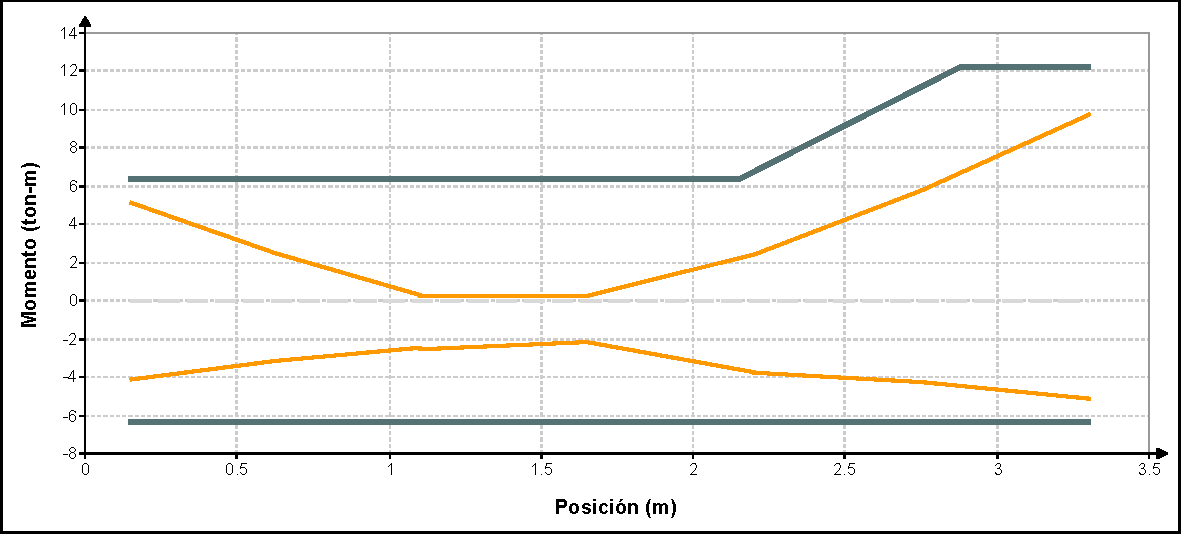
\includegraphics[scale=0.6]{IMAGENES/capb.pdf}
    %\caption*{\small Fuente: \it \cite{cordova2015}}
    \label{vigm}
\end{figure}

\textit{Desarrollo de ganchos estándar en tracción}
\begin{theo}[Art. 12.5.1 y 12.5.2 :]{thm:ca1}
La longitud de desarrollo para barras corrugadas en tracción que terminen en un gancho estándar (véase 7.1), se debe calcular según 12.5.2 y los factores de modificación de 12.5.3, pero no debe ser menor que el menor valor entre  8 db  y 150 mm.\\
Para las barras corrugadas, $l_{dg} $ se calcula con $\psi_{e}$ igual a 1,2 
para refuerzo con recubrimiento epóxico y $\lambda$ igual a 1,3 para concretos livianos.  Para otros casos, $\psi_{e}$  y $\lambda$  deben tomarse igual a 1,0
\end{theo}
\FPeval{\ldg}{round(\fy*0.075*\dbcm/(\rc),2)}
\begin{flalign}
l_{dg}&=\left (0.075 \cdot \psi_{e}\cdot \lambda\cdot  f_{y}/\sqrt{f_{c}^{'}} \right )d_{b}\\
l_{dg}&=\left (0.075 \cdot 1.00 \cdot 1.00 \cdot  \fy/\sqrt{\fc} \right )\dbcm=\ldg\mathrm{~cm}\notag
\end{flalign}
\noindent Se concluye que se necesita por lo menos 40cm para que el acero de 5/8" desarrolle con gancho estándar, dado que la viga del eje 6 llega a columnas con peraltes de 55cm se asegura el anclaje sin necesidad de alguna consideración especial como se menciona en 12.5.3.
\begin{figure}[h!]
    \centering
    \caption{desarrollo de gancho estándar}
    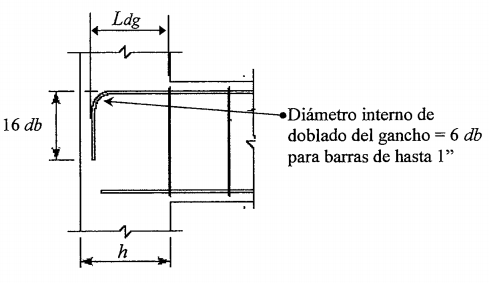
\includegraphics[scale=1]{IMAGENES/gancho.PNG}
    \caption*{\small Fuente: \it \cite{pasino2011}}
    \label{vigm}
\end{figure}
\subsubsection{Refuerzo mínimo de elementos sujetos a flexión Art. 10.5}
\begin{theo}[Art. 10.5.1 E-060 :]{thm:ca1}
En cualquier sección de un elemento estructural - excepto en zapatas y losas macizas - sometidos a flexión, donde por el análisis se requiere refuerzo de acero en tracción, el área de acero que se proporcione será la necesaria para que la resistencia de diseño de la sección sea por lo menos 1.2 veces el momento de agrietamiento de la sección bruta $M_{cr}$ $\left ( \phi\;M_{n}\geq1.2\;M_{cr} \right )$.
\end{theo}
\vspace{-0.8cm}
\begin{flalign}
\textup{Ecu.(9.12) E-060:}\hspace{4.3cm} f_{r}=2\sqrt{f_{c}^{'}}&&
\end{flalign}
\myequations{Modulo de ruptura del concreto}
\vspace{-1.5cm}
\begin{flalign}
\textup{Ecu.(9.11) E-060:}\hspace{4.3cm} M_{cr}=\frac{f_{r}\cdot I_{g}}{Y_{t}}&&
\end{flalign}
\myequations{Momento de agrietamiento}
\vspace{-0.8cm}
\noindent La norma el articulo 10.5.2 también menciona que el acero mínimo en secciones rectangulares no debe ser menor que la ecuación \eqref{min}, \cite{pasino2011} menciona que lo anterior implica que el momento resistente es aproximadamente 1.5 veces el momento de agrietamiento por lo que se cumple con lo dispuesto en 10.5.
\begin{flalign}
\textup{Ecu.(10.3) E-060:}\hspace{3.6cm}A_{s}=\frac{0.7\sqrt{f_{c}^{'}}}{f_{y}}\cdot b_{w}\cdot d&&\label{min}
\end{flalign}
\FPeval{\rb}{round((0.7*\rc*\bv*\defe)/\fy,2)}
\FPeval{\pmin}{round((0.7*\rc)/\fy,4)}
\begin{equation*}
A_{s}=\frac{0.7\sqrt{\fc}}{\fy}\cdot \bv\cdot \defe=\pmin\cdot \bv\cdot \defe=\rb\;\mathrm{cm}^{2}
\end{equation*}
%$\centering \displaystyle A_{s}=\frac{0.7\sqrt{\fc}}{\fy}\cdot \bv\cdot \defe=\rb\;\mathrm{cm}^{2}$\\

%\begin{theo}[Art. 10.5.3 E-060 :]{thm:ca1}
    %No es necesario satisfacer los requisitos de 10.5.1 y 10.5.2, si en cada sección del elemento el área de acero en tracción proporcionada es al menos un tercio superior a la requerida por análisis.
%\end{theo}
\noindent
El acero colocado es mayor al mínimo dispuesto por la norma.
\subsubsection{Refuerzo máximo de elementos sujetos a flexión}
\begin{theo}[Art. 10.3.4 E-060 :]{thm:ca1}
En elementos no preesforzados sujetos a flexión o flexocompresión en los cuales $\phi P_{n}$ sea menor que 0,1 f’c Ag, el refuerzo de acero en tracción no deberá exceder de 0,75 Asb, donde Asb es la cantidad de acero en tracción que produce la falla balanceada en la sección, definida en 10.3.2.
\end{theo}

\begin{theo}[Cuantía balanceada Art. 10.3.2 E-060 :]{thm:ca1}
La condición de falla balanceada se produce en una sección transversal cuando el refuerzo en tracción alcanza la deformación unitaria correspondiente a fy al mismo tiempo que el concreto en compresión alcanza su deformación unitaria máxima utilizable de 0.003. Este criterio es general y se aplica a secciones de cualquier forma sin acero en compresión o con él.
\end{theo}
\begin{align}
\rho_{b}&=\frac{0,85 \cdot f_{c}^{\prime} \cdot \beta_{1}}{f_{y}}\left(\frac{\varepsilon_{c}}{\varepsilon_{y}+\varepsilon_{c}}\right)\\
\rho_{\max }&=0,75\;\rho_{b}
%\label{max}
\end{align}
\begin{figure}[h!]
    \centering
    \caption{Cuantía balanceada}
    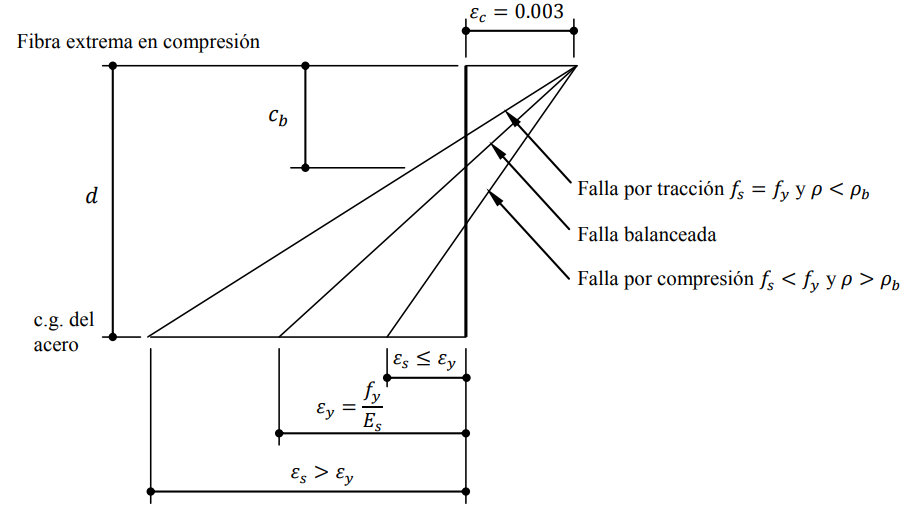
\includegraphics[scale=0.6]{IMAGENES/d1.PNG}
    \caption*{\small Fuente: \it \cite{cordova2015}}
    \label{ver}
\end{figure}
\FPeval{\rcc}{round((0.85*\fc*0.85*0.003)/(\fy*(0.003+0.0021)),4)}
\FPeval{\rcd}{round(0.75*\rcc,3)}
\newpage
\noindent
Para $f_{c}^{\prime}=210\;\mathrm{cm}^{2}$ y $f_{y}=4200\;\mathrm{cm}^{2}$ la cuantía balanceada y máxima sera:
\begin{gather*}
\rho_{b}=\frac{0,85 \cdot \fc \cdot 0.85}{\fy}\left(\frac{0.003}{0.0021+0.003}\right)=\rcc\\
\rho_{\max }=0,75\cdot\rcc=\rcd
%\label{max}
\end{gather*}
\noindent La cuantía colocada esta muy por debajo de la máxima dispuesta por la norma.
%\newpage
\subsubsection{Disposición del acero del refuerzo longitudinal (Art. 21.4.4 y 25.5.2)}
\begin{theo}[Art. 21.4.4.1 y 21.5.2.1 :]{thm:ca1}
\textit{Vigas en sistemas de muros}\\
Deberá existir refuerzo continuo a todo lo largo de la viga, constituido por dos barras tanto en la cara superior como en la inferior, con un área de acero no menor de la especificada en 10.5. No se aplicará lo dispuesto en 10.5.3.\\
\textit{Vigas de sistemas duales o pórticos}\\
Adicionalmente a lo anterior la cuantía de refuerzo en tracción no deberá exceder de 0,025.
\end{theo}
\begin{theo}[Art. 21.4.4.3 y 21.5.2.2 :]{thm:ca1}
La resistencia a momento negativo y positivo en cualquier sección a lo largo de la longitud del elemento deben ser mayores de un cuarto de la máxima resistencia a momento proporcionada en la cara de cualquiera de los nudos.\\
\textit{Vigas en sistemas de muros}\\
La resistencia a momento positivo en la cara del nudo no debe ser menor que un tercio de la resistencia a momento negativo provista en dicha cara.\\
\textit{Vigas de sistemas duales o pórticos}\\
La resistencia a momento positivo en la cara del nudo no debe ser menor que la mitad de la resistencia a momento negativo provista en dicha cara.
\end{theo}

\begin{figure}[h!]
    \centering
    \caption{Requisitos del refuerzo longitudinal en vigas}
    \subfigure[Sistemas de muros]{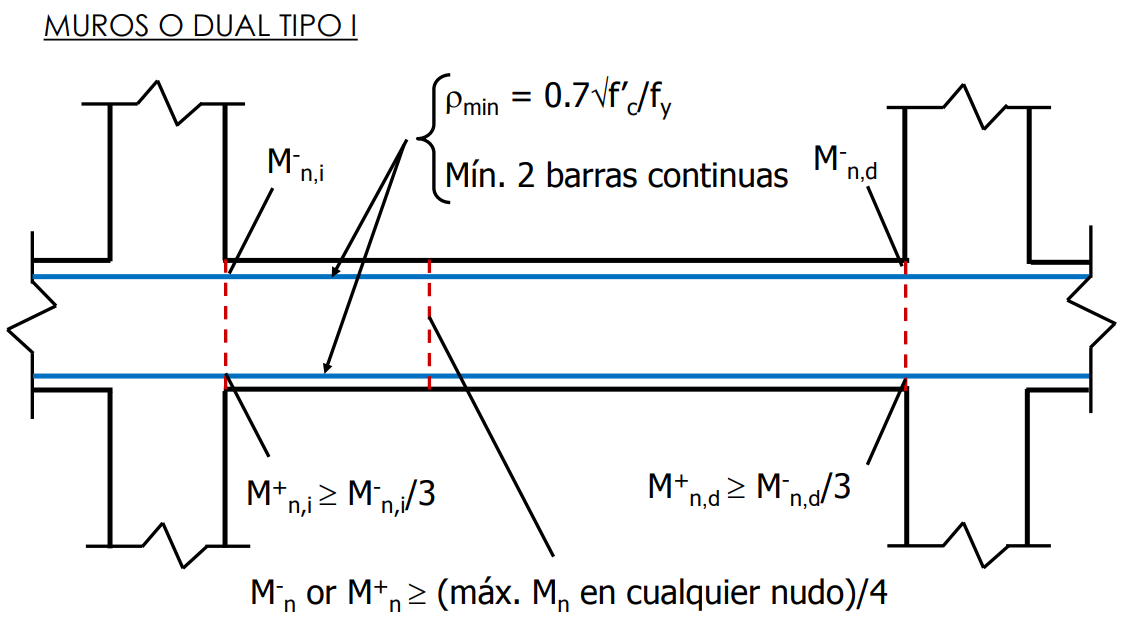
\includegraphics[width=90mm]{IMAGENES/d2.PNG}}\hspace{0mm}
    \subfigure[Sistemas de pórticos o duales]{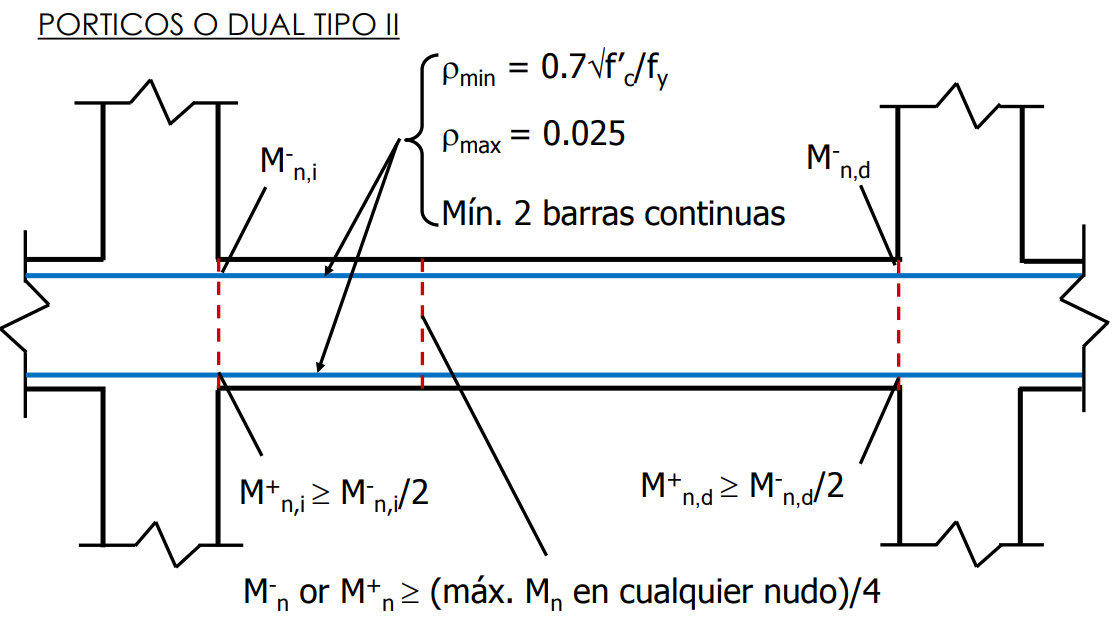
\includegraphics[width=90mm]{IMAGENES/d3.PNG}}
    \caption*{Fuente: \cite{CAPUCP}}
    \label{reqv}
\end{figure}

\noindent En la dirección X se trata de un sistema de muros por lo que se exige que la resistencia a momento mínima en un nudo sea por lo menos la tercera parte del máximo, tal condición se cumple dado que el momento $\phi M_{n,1}$ es mayor que el 50\% que $\phi M_{n,2}$.

\subsubsection{Diseño a corte por capacidad}
\begin{theo}[Art. 21.4.3 y 21.5.4.1:]{thm:ca1}
\textit{Vigas en sistemas de muros}\\
La cortante de diseño para vigas que resistan efectos sísmicos se calculara como la suma del cortante asociado con el desarrollo de los momentos nominales (Mn) del elemento en cada extremo restringido de la luz libre y el cortante isostático calculado para las cargas de gravedad tributarias amplificadas.\\
El cortante máximo obtenido de las combinaciones de carga de diseño de 9.2.3 con un factor de amplificación para los valores del sismo igual a 2,5.\\
\textit{Vigas en sistemas de pórticos o duales}\\
La fuerza cortante de diseño, Vu, de los elementos en flexión, deberá determinarse a partir de la suma de las fuerzas cortantes asociadas con el desarrollo de las resistencias probables en flexión (Mpr = 1,25 Mn) en los extremos de la luz libre del elemento y la fuerza cortante isostática calculada para las cargas de gravedad tributarias amplificadas.
\end{theo}
\begin{align}
V_{u}=\frac{M_{p, i s q}+M_{p, d e r}}{l_{n}} \pm W_{u} \cdot \frac{l_{n}}{2}
\end{align}
\noindent Calculo de la carga distribuida sobre la viga:
\FPset\plosa{0.3}
\FPset\alosa{3.2}
\FPset\wpt{0.1}
\FPset\wlosa{0.2}
\FPeval{\wviga}{round((\plosa+\wpt)*\alosa+2.4*\bv*\h/10000,2)}
\FPeval{\wvigav}{round((\wlosa)*\alosa,2)}
\FPeval{\wvigau}{round(1.25*(\wviga+\wvigav),2)}
\begin{itemize}
  \item Peso distribuido de la losa aligerada: $w_{\text {alig }}=\plosa \mathrm{~ton} / \mathrm{m}^{2}$
  \item Ancho tributario de la losa aligerada: $A_{t}=\alosa \mathrm{~m}$
  \item Sobrecarga muerta por piso terminado: $w_{p t}=\wpt \mathrm{~ton}/ \mathrm{m}^{2}$
  \item Carga viva sobre losas: $w_{sc}=\wlosa \mathrm{~ton}/\mathrm{m}^{2}$
\end{itemize}
\newpage
\noindent Carga muerta total distribuida sobre la viga:
\begin{center}
$W_{c m}=b \cdot h \cdot \gamma_{c}+\left(w_{a l i g}+w_{p t}\right) \cdot A_{t}=\wviga \text {~ton}/{m}$
\end{center}
\noindent Carga viva distribuida  sobre la viga:
\begin{center}
$W_{c v}=w_{sc} \cdot A_{t}=\wlosa\cdot\alosa=\wvigav \text {~ton}/{m}$
\end{center}
\noindent Carga ultima sobre la viga:
\begin{center}
$W_{u}=1,25 \cdot\left(W_{c m}+W_{c v}\right)=1,25 \cdot\left(\wviga+\wvigav\right)=\wvigau \text {~ton}/{m}$
\end{center}
%\newpage
\begin{figure}[h!]
    \centering
    \subfigure[Sistemas de muros]{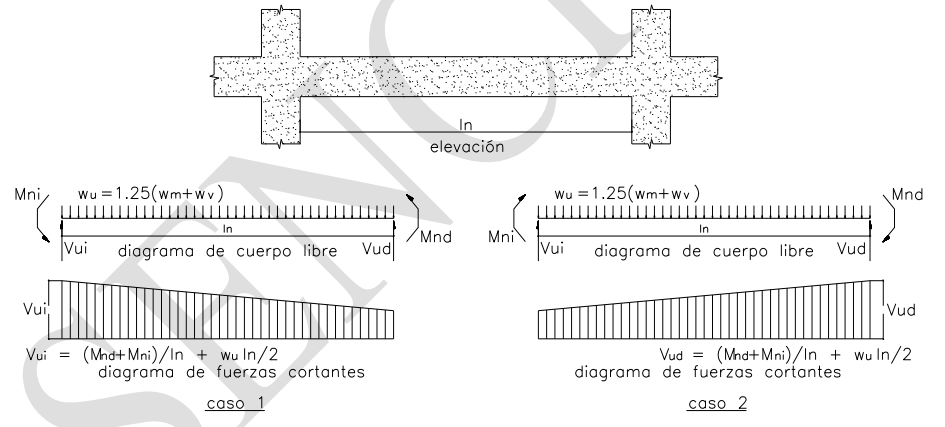
\includegraphics[width=130mm]{IMAGENES/d4.PNG}}\hspace{0mm}
    \subfigure[Sistemas de pórticos o duales]{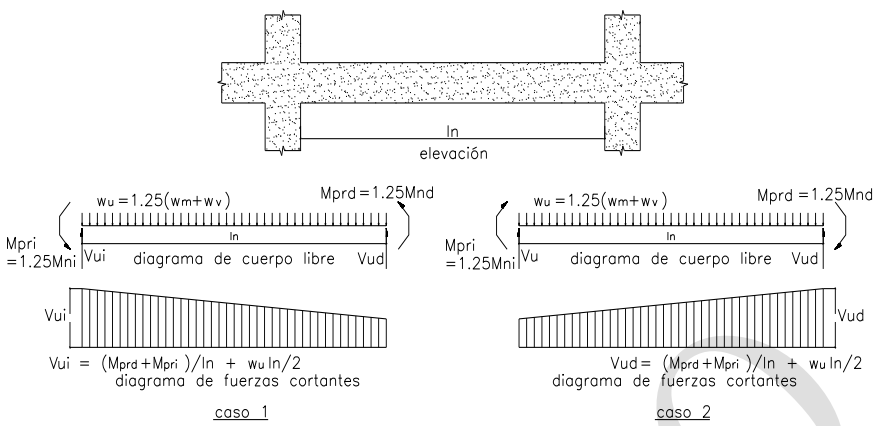
\includegraphics[width=130mm]{IMAGENES/d8.PNG}}
    \caption{Diseño por corte capacidad en vigas}
    \label{reqv}
\end{figure}
\FPeval{mncoru}{round(mncor/0.9,2)}
\FPeval{mnderu}{round(mnder/0.9,2)}
\newpage
\noindent CASO 1:\\
Momento negativo en el extremo izquierdo:
\begin{center}
$M_{n,isq-}=\mncor/0.9=\mncoru\;\mathrm{~ton.m}$
\end{center}
Momento positivo en el extremo derecho:
\begin{center}
$M_{n,der+}=M_{n,isq-}=\mncoru\;\mathrm{~ton.m}$
\end{center}
Cortante por capacidad:
\FPeval{\va}{round(2*\mncoru/\ln+\wvigau*\ln*0.5,2)}
\FPeval{\vb}{round(2*\mncoru/\ln-\wvigau*\ln*0.5,2)}
\begin{align*}
V_{1,1}&=\frac{2\cdot\mncoru}{\ln} + \wvigau  \cdot \frac{\ln}{2}=\va\text {~ton}\\
V_{1,2}&=\frac{2\cdot\mncoru}{\ln} - \wvigau  \cdot \frac{\ln}{2}=\vb\text {~ton}
\end{align*}
CASO 2:\\
\FPeval{\vc}{round((\mnderu+\mncoru)/\ln+\wvigau*\ln*0.5,2)}
\FPeval{\vd}{round((\mnderu+\mncoru)/\ln-\wvigau*\ln*0.5,2)}
Momento positivo en el extremo izquierdo: 
\begin{center}
$M_{n,isq-}=\mncor/0.9=\mncoru\;\mathrm{~ton.m}$
\end{center}
Momento negativo en el extremo derecho: 
\begin{center}
$\displaystyle M_{n,der+}=\mnder/0.9=\mnderu\;\mathrm{~ton.m}$
\end{center}
Cortante por capacidad:
\begin{align*}
V_{2,1}=\frac{\mncoru+\mnderu}{\ln} + \wvigau  \cdot \frac{\ln}{2}=\vc\text {~ton}\\
V_{2,2}=\frac{\mncoru+\mnderu}{\ln} - \wvigau  \cdot \frac{\ln}{2}=\vd\text {~ton}
\end{align*}
En la figura \ref{cor} se muestra las cortantes por capacidad y dado que se trata de una viga perteneciente a un sistema de muros también se muestra las cortantes máximas para las combinaciones de sismo con un factor de amplificación de 2,5 como se menciona en 21.4.3.
\newpage
\begin{figure}[h!]
    \centering
    \caption{Envolvente de cortantes}
    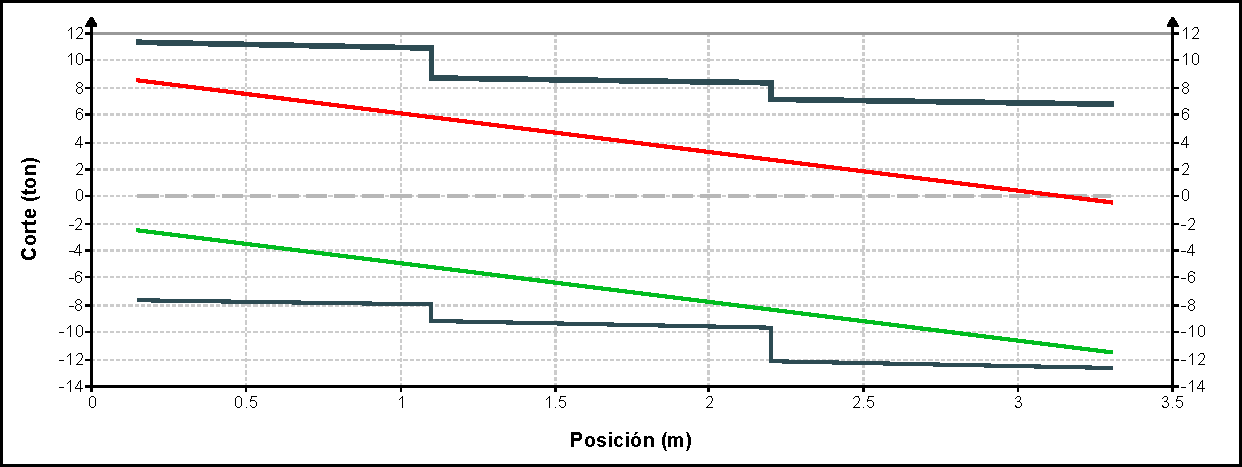
\includegraphics[scale=0.7]{IMAGENES/corta.pdf}
    %\caption*{\small Fuente: \it \cite{cordova2015}}
    \label{cor}
\end{figure}

\subsubsection{Disposiciones del refuerzo transversal en las zonas de confinamiento de vigas}
En ambos extremos del elemento deben disponerse estribos cerrados de confinamiento en longitudes iguales a dos veces el peralte del elemento medido desde la cara del elemento de apoyo hacia el centro de la luz, ya que en estas zonas puede ocurrir fluencia por flexión debido a desplazamientos laterales inelásticos de la estructura.
\begin{theo}[Art. 21.4.4.4 y 21.5.3.2 :]{thm:ca1}
\textit{Vigas en sistemas de muros}\\
El primer estribo cerrado de confinamiento debe estar situado a no más de 100 mm de la cara del elemento de apoyo.  Los estribos serán como mínimo de 8 mm de diámetro para barras longitudinales de hasta 5/8" de diámetro, de 3/8" para barras longitudinales de hasta  1" de diámetro y de 1/2" para barras longitudinales de mayor diámetro. \\
\textit{Vigas en sistemas de pórticos o duales}\\
Los estribos serán como mínimo de 3/8" para barras longitudinales de hasta 1" de diámetro y de  1/2"  para  barras  longitudinales  de  mayor  diámetro. El primer  estribo  cerrado  de confinamiento debe estar situado a no más de 50 mm de la cara del elemento de apoyo.
\end{theo}
\newpage
\noindent El espaciamiento del refuerzo transversal en vigas de sistemas de muros no debe exceder el menor de:
%\vspace{-0.3cm}
\begin{enumerate}
\item[] (a): $d / 4 \geq 15 \mathrm{~cm}$
\item[] (b): $10d_{b}$
\item[] (c): $24d_{e}$
\item[] (d): $30 \mathrm{~cm}$
\end{enumerate}
\noindent
Donde:\\
$d$: Peralte efectivo\\
$d_{b}$: Diámetro de la barra longitudinal de menor diámetro\\
$d_{e}$: Diámetro del estribo\\
En vigas de sistemas de pórticos o duales la condición (b) cambia por: $8d_{b}$ y se debe cumplir que en las zonas de confinamiento, la distancia horizontal entre las ramas verticales del refuerzo transversal (estribos cerrados y/o grapas suplementarias) no deberá exceder de 300 mm (Art. 21.5.3.3)\\
Para el presente caso se tiene:
\FPeval{\dcuar}{round(\defe/4,2)}
\FPeval{\conb}{round(\vacm*10,2)}
\FPeval{\conc}{round(\estcm*24,2)}
\FPeval{\lcon}{round(\h*2/100,2)}
\begin{enumerate}
\item[] (a): $d / 4=\dcuar\mathrm{~cm} \geq 15 \mathrm{~cm}$
\item[] (b): $10d_{b}=\conb\mathrm{~cm}$
\item[] (c): $24d_{e}=\conc\mathrm{~cm}$
\item[] (d): $30 \mathrm{~cm}$
\end{enumerate}
Por lo tanto la separación final de estribos dentro de la longitud de confinamiento $2h=\lcon\mathrm{~m}$ sera 10cm.
\newpage
\subsubsection{Disposiciones del refuerzo transversal fuera de la zona de confinamiento en vigas}
\begin{theo}[Art. 21.4.4.4 y 21.5.3.2 :]{thm:ca1}
\textit{Vigas en sistemas de muros}\\
Los estribos deben estar espaciados a no más de 0,5d a lo largo de la longitud del elemento. En todo el elemento la separación de los estribos, no deberá ser mayor que la requerida por fuerza cortante. \\
\textit{Vigas en sistemas de pórticos o duales}\\
Fuera  de  las  zonas  de  confinamiento,  deben  colocarse  estribos  cerrados con  ganchos sísmicos en ambos extremos, espaciados a no más de d/2 en toda la longitud del elemento. En todo el elemento la separación de los estribos, no será mayor que la requerida por fuerza cortante.
\end{theo}
\FPeval{\sepf}{round(\defe/2,2)}
\noindent La separación del refuerzo transversal fuera de la zona de confinamiento sera: $s=d/2=\sepf\approx20\mathrm{~cm}$\\
Por lo tanto, el diseño final a cortante de la viga será:
\begin{center}
$1 @ 5 \mathrm{~cm}, 10 @ 10 \mathrm{~cm}$, Rto.@20cm   
\end{center}
\subsubsection{Disposiciones adicionales para vigas en sistemas de pórticos o duales}
\begin{theo}[Art. 21.4.4.4 y 21.5.3.2 :]{thm:ca1}
Sólo se permiten empalmes por traslape del refuerzo de flexión cuando se proporcionan estribos de confinamiento o espirales en la toda longitud del empalme.   El espaciamiento del refuerzo transversal que envuelve las barras traslapadas no debe exceder el menor de d/4 ó 150 mm.
\end{theo}
\newpage
\noindent No deben emplearse empalmes por traslape:
\begin{enumerate}
\item[] (a): dentro los nudos
\item[] (b): en una distancia de dos veces el peralte del elemento medida desde la cara del nudo
\item[] (c): donde  el  análisis  indique  fluencia  por  flexión  del  refuerzo causada  por  los desplazamientos laterales inelásticos del pórtico.
\end{enumerate}
\begin{figure}[h!]
    \centering
      \caption{Resumen de requisitos del refuerzo transversal en vigas}
    \subfigure[Sistemas de muros]{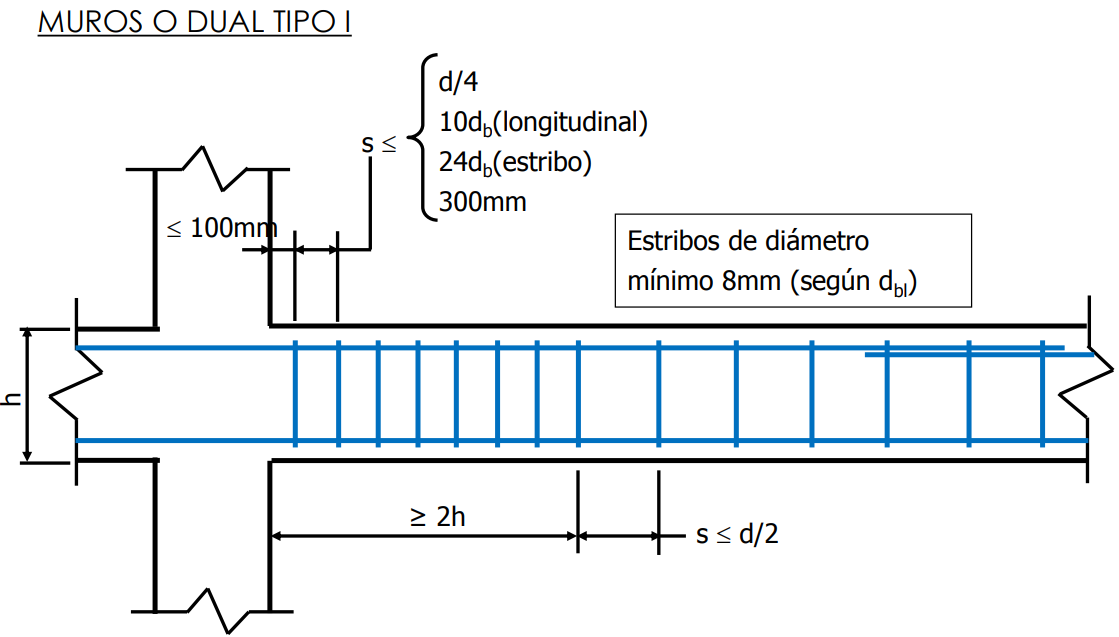
\includegraphics[width=95mm]{IMAGENES/d6.PNG}}\hspace{0mm}
    \subfigure[Sistemas de pórticos o duales]{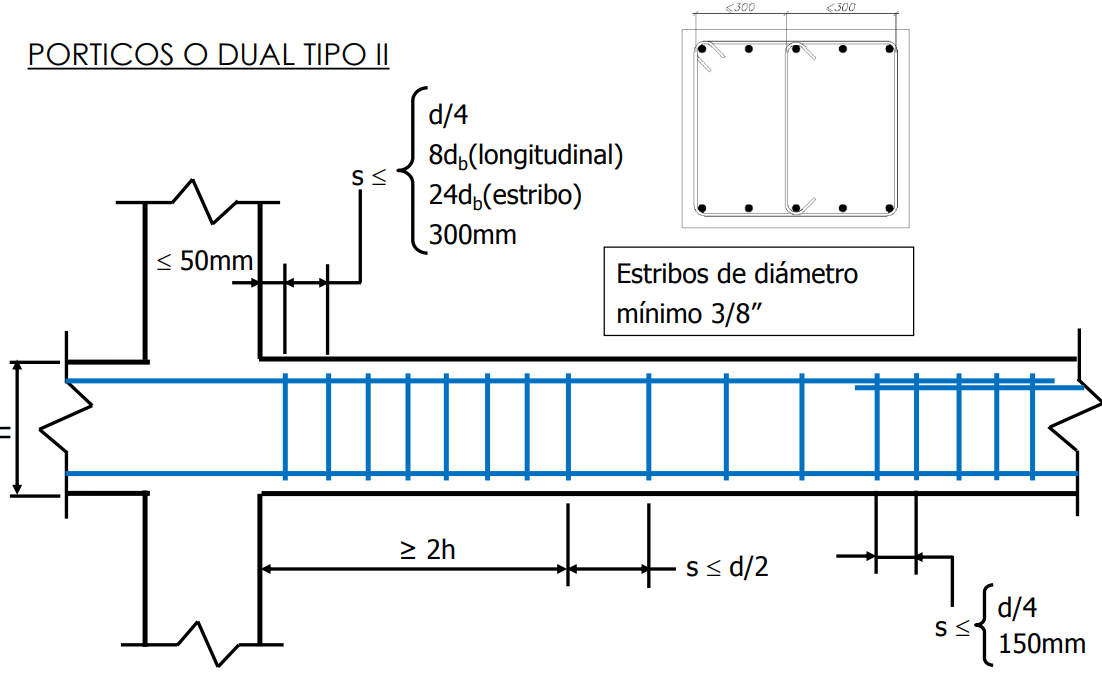
\includegraphics[width=95mm]{IMAGENES/d7.PNG}}
    \caption*{Fuente: \cite{CAPUCP}}
    \label{reqv}
\end{figure}
\subsubsection{Resistencia a corte Cap. 11}
La resistencia a cortante de la sección, concreto y acero transversal esta dado respectivamente por:
\begin{flalign}
&\textup{Ecu.(11.1) y (11.2) E-060:}&\phi V_{n}&=\phi_{c} \cdot\left(V_{c}+V_{e}\right)&&\\
&\textup{Ecu.(11.3) E-060:}&V_{c}&=0,53 \cdot \sqrt{f_{c}^{\prime}} \cdot b \cdot d&&\label{vc}\\
&\textup{Ecu.(11.15) E-060:}&V_{e}&=\frac{n \cdot A_{s h} \cdot f_{y} \cdot d}{s}&&\label{vmax}
\end{flalign}
\noindent
Donde:\\
$n$ : Numero de ramas de estribos\\
$A_{s h}:$ Área del acero transversal\\
$s:$ Separación del refuerzo transversal\\
La cortante máxima que pueden tomar los estribos esta dado por:
\begin{flalign}
&\textup{Art. 11.5.7.9 E-060:}&V_{e, \max }&=2,1 \cdot \sqrt{f_{c}^{\prime}} \cdot b \cdot d&&
\end{flalign}
\noindent
%Verificación de la capacidad a fuerza cortante de la viga:\\
Cortante resistente por el concreto según \ref{vc}:
\FPeval{\vcon}{round(0.53*\rc*\bv*\defe/1000,2)}
\begin{center}
$V_{c}=0,53 \cdot \sqrt{f_{c}^{\prime}} \cdot b \cdot d=0,53 \cdot \sqrt{\fc} \cdot \bv \cdot \defe=\vcon\mathrm{~ton}$
\end{center}
Cortante resistente por los estribos en la zona de confinamiento:
\FPeval{\ves}{round(2*0.71*\fy*\defe/10000,2)}
\begin{center}
$\displaystyle V_{e,1}=\frac{n \cdot A_{s h} \cdot f_{y} \cdot d}{s}=\frac{2 \cdot 0,71 \cdot 4200 \cdot \defe}{10}=\ves \mathrm{ton}$
\end{center}
Cortante resistente por los estribos fuera de la zona de confinamiento:
\FPeval{\vesf}{round(2*0.71*\fy*\defe/20000,2)}
\begin{center}
$\displaystyle V_{e,2}=\frac{n \cdot A_{s h} \cdot f_{y} \cdot d}{s}=\frac{2 \cdot 0,71 \cdot 4200 \cdot \defe}{20}=\vesf \mathrm{ton}$
\end{center}
Cortante máxima que pueden soportar los estribos:
\FPeval{\vmax}{round(2.1*\rc*\bv*\defe/1000,2)}
\begin{center}
$\displaystyle V_{e, \max }=2,1 \cdot \sqrt{\fc} \cdot \bv \cdot \defe=\vmax\mathrm{ton}>V_{e}=\ves\mathrm{ton}$ 
\end{center}
Cortante nominal en la zona de confinamiento:
\FPeval{\vnom}{round((\vcon+\ves)*0.85,2)}
\begin{center}
$\displaystyle \phi V_{n,1}=\phi_{c} \cdot\left(V_{c}+V_{e}\right)=0,85 \cdot(\vcon+\ves)=\vnom\mathrm{Ton}$
\end{center}
Cortante nominal fuera de la zona de confinamiento:
\FPeval{\vnomf}{round((\vcon+\vesf)*0.85,2)}
\begin{center}
$\displaystyle \phi V_{n,2}=\phi_{c} \cdot\left(V_{c}+V_{e}\right)=0,85 \cdot(\vcon+\vesf)=\vnomf\mathrm{ton}$
\end{center}
Según el artículo 11.1.3.1 se permite diseñar los elementos para la fuerza cortante a una distancia $d$ de la cara.\\
Como se aprecia en la figura \ref{corcap} al cumplir las disposiciones del refuerzo transversal se cumple holgadamente con las solicitaciones máximas de la viga a cortante.
\begin{figure}[h!]
    \centering
    \caption{Demanda capacidad a corte de la viga}
    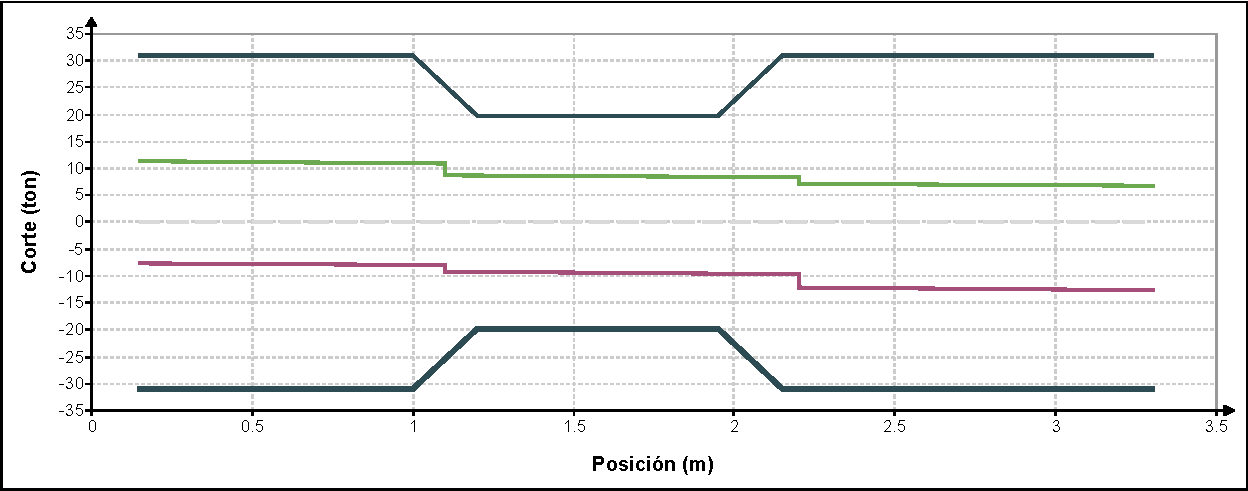
\includegraphics[scale=0.7]{IMAGENES/capcor.pdf}
    %\caption*{\small Fuente: \it \cite{cordova2015}}
    \label{corcap}
\end{figure}

\begin{figure}[h!]
    \caption{Esquema de armado de viga EJE 6 tramo A-B}
    \centering
    



\tikzset{every picture/.style={line width=0.75pt}} %set default line width to 0.75pt        

\begin{tikzpicture}[x=0.75pt,y=0.75pt,yscale=-0.85,xscale=0.85]
%uncomment if require: \path (0,279); %set diagram left start at 0, and has height of 279

%Straight Lines [id:da8216381485043296] 
\draw    (20,100) -- (680,100) ;
%Straight Lines [id:da3359330334123778] 
\draw    (20,190) -- (680,190) ;
%Straight Lines [id:da5424331560324562] 
\draw    (20,100) -- (20,60) ;
%Straight Lines [id:da018993591999090897] 
\draw    (20,230) -- (20,190) ;
%Straight Lines [id:da6552270957993611] 
\draw    (680,100) -- (680,60) ;
%Straight Lines [id:da07733863212657455] 
\draw    (680,230) -- (680,201.5) -- (680,190) ;
%Straight Lines [id:da7882319327917733] 
\draw [color={rgb, 255:red, 144; green, 19; blue, 254 }  ,draw opacity=1 ][line width=1.5]    (0,110) -- (700,110) ;
%Straight Lines [id:da54894949033232] 
\draw [color={rgb, 255:red, 144; green, 19; blue, 254 }  ,draw opacity=1 ][line width=1.5]    (0,180) -- (700,180) ;
%Straight Lines [id:da26484967516193847] 
\draw [color={rgb, 255:red, 126; green, 211; blue, 33 }  ,draw opacity=1 ][line width=1.5]    (30,105) -- (30,185) ;
%Straight Lines [id:da5737580593612992] 
\draw [color={rgb, 255:red, 126; green, 211; blue, 33 }  ,draw opacity=1 ][line width=1.5]    (70,105) -- (70,185) ;
%Straight Lines [id:da6277522044473443] 
\draw [color={rgb, 255:red, 126; green, 211; blue, 33 }  ,draw opacity=1 ][line width=1.5]    (50,105) -- (50,185) ;
%Straight Lines [id:da13849105923311478] 
\draw [color={rgb, 255:red, 126; green, 211; blue, 33 }  ,draw opacity=1 ][line width=1.5]    (90,105) -- (90,185) ;
%Straight Lines [id:da11541108338806993] 
\draw [color={rgb, 255:red, 126; green, 211; blue, 33 }  ,draw opacity=1 ][line width=1.5]    (110,105) -- (110,185) ;
%Straight Lines [id:da7071575489896418] 
\draw [color={rgb, 255:red, 126; green, 211; blue, 33 }  ,draw opacity=1 ][line width=1.5]    (130,105) -- (130,185) ;
%Straight Lines [id:da6966211342573374] 
\draw [color={rgb, 255:red, 126; green, 211; blue, 33 }  ,draw opacity=1 ][line width=1.5]    (150,105) -- (150,185) ;
%Straight Lines [id:da798706719132402] 
\draw [color={rgb, 255:red, 126; green, 211; blue, 33 }  ,draw opacity=1 ][line width=1.5]    (170,105) -- (170,185) ;
%Straight Lines [id:da3276906292450714] 
\draw [color={rgb, 255:red, 126; green, 211; blue, 33 }  ,draw opacity=1 ][line width=1.5]    (190,105) -- (190,185) ;
%Straight Lines [id:da2731164518940632] 
\draw [color={rgb, 255:red, 126; green, 211; blue, 33 }  ,draw opacity=1 ][line width=1.5]    (210,105) -- (210,185) ;
%Straight Lines [id:da283115192526185] 
\draw [color={rgb, 255:red, 126; green, 211; blue, 33 }  ,draw opacity=1 ][line width=1.5]    (230,105) -- (230,185) ;
%Straight Lines [id:da8440765293574195] 
\draw [color={rgb, 255:red, 72; green, 145; blue, 251 }  ,draw opacity=1 ][line width=1.5]    (270,105) -- (270,185) ;
%Straight Lines [id:da36110068367148673] 
\draw [color={rgb, 255:red, 72; green, 145; blue, 251 }  ,draw opacity=1 ][line width=1.5]    (310,105) -- (310,185) ;
%Straight Lines [id:da3837355756909533] 
\draw [color={rgb, 255:red, 72; green, 145; blue, 251 }  ,draw opacity=1 ][line width=1.5]    (350,105) -- (350,185) ;
%Straight Lines [id:da26375379887302697] 
\draw [color={rgb, 255:red, 72; green, 145; blue, 251 }  ,draw opacity=1 ][line width=1.5]    (390,105) -- (390,185) ;
%Straight Lines [id:da867101053954658] 
\draw [color={rgb, 255:red, 72; green, 145; blue, 251 }  ,draw opacity=1 ][line width=1.5]    (430,105) -- (430,185) ;
%Straight Lines [id:da7898101820337782] 
\draw [color={rgb, 255:red, 126; green, 211; blue, 33 }  ,draw opacity=1 ][line width=1.5]    (470,105) -- (470,185) ;
%Straight Lines [id:da7882178509824598] 
\draw [color={rgb, 255:red, 126; green, 211; blue, 33 }  ,draw opacity=1 ][line width=1.5]    (510,105) -- (510,185) ;
%Straight Lines [id:da17202188816739783] 
\draw [color={rgb, 255:red, 126; green, 211; blue, 33 }  ,draw opacity=1 ][line width=1.5]    (490,105) -- (490,185) ;
%Straight Lines [id:da7081343310587527] 
\draw [color={rgb, 255:red, 126; green, 211; blue, 33 }  ,draw opacity=1 ][line width=1.5]    (530,105) -- (530,185) ;
%Straight Lines [id:da6424376057537702] 
\draw [color={rgb, 255:red, 126; green, 211; blue, 33 }  ,draw opacity=1 ][line width=1.5]    (550,105) -- (550,185) ;
%Straight Lines [id:da720929820876927] 
\draw [color={rgb, 255:red, 126; green, 211; blue, 33 }  ,draw opacity=1 ][line width=1.5]    (570,105) -- (570,185) ;
%Straight Lines [id:da9208625514397295] 
\draw [color={rgb, 255:red, 126; green, 211; blue, 33 }  ,draw opacity=1 ][line width=1.5]    (590,105) -- (590,185) ;
%Straight Lines [id:da5102013133871048] 
\draw [color={rgb, 255:red, 126; green, 211; blue, 33 }  ,draw opacity=1 ][line width=1.5]    (610,105) -- (610,185) ;
%Straight Lines [id:da40022767303945894] 
\draw [color={rgb, 255:red, 126; green, 211; blue, 33 }  ,draw opacity=1 ][line width=1.5]    (630,105) -- (630,185) ;
%Straight Lines [id:da08442925729566886] 
\draw [color={rgb, 255:red, 126; green, 211; blue, 33 }  ,draw opacity=1 ][line width=1.5]    (650,105) -- (650,185) ;
%Straight Lines [id:da765109025040853] 
\draw [color={rgb, 255:red, 126; green, 211; blue, 33 }  ,draw opacity=1 ][line width=1.5]    (670,105) -- (670,185) ;
%Straight Lines [id:da8837836561141847] 
\draw    (70,85) -- (90,85) ;
\draw [shift={(90,85)}, rotate = 180] [color={rgb, 255:red, 0; green, 0; blue, 0 }  ][line width=0.75]    (0,5.59) -- (0,-5.59)   ;
\draw [shift={(70,85)}, rotate = 180] [color={rgb, 255:red, 0; green, 0; blue, 0 }  ][line width=0.75]    (0,5.59) -- (0,-5.59)   ;
%Straight Lines [id:da16273587413241297] 
\draw    (230,85) -- (270,85) ;
\draw [shift={(270,85)}, rotate = 180] [color={rgb, 255:red, 0; green, 0; blue, 0 }  ][line width=0.75]    (0,5.59) -- (0,-5.59)   ;
\draw [shift={(230,85)}, rotate = 180] [color={rgb, 255:red, 0; green, 0; blue, 0 }  ][line width=0.75]    (0,5.59) -- (0,-5.59)   ;
%Straight Lines [id:da48768573746932486] 
\draw    (20,205) -- (30,205) ;
\draw [shift={(30,205)}, rotate = 180] [color={rgb, 255:red, 0; green, 0; blue, 0 }  ][line width=0.75]    (0,5.59) -- (0,-5.59)   ;
\draw [shift={(20,205)}, rotate = 180] [color={rgb, 255:red, 0; green, 0; blue, 0 }  ][line width=0.75]    (0,5.59) -- (0,-5.59)   ;
%Straight Lines [id:da8748711892951206] 
\draw [color={rgb, 255:red, 249; green, 59; blue, 59 }  ,draw opacity=1 ][line width=1.5]    (480,120) -- (700,120) ;
%Straight Lines [id:da36112134786222017] 
\draw [color={rgb, 255:red, 246; green, 169; blue, 38 }  ,draw opacity=1 ][line width=1.5]    (530,130) -- (700,130) ;
%Curve Lines [id:da6931974948329667] 
\draw    (450,110) .. controls (458.27,88.82) and (437.05,80.74) .. (401.63,80.03) ;
\draw [shift={(400,80)}, rotate = 0.79] [color={rgb, 255:red, 0; green, 0; blue, 0 }  ][line width=0.75]    (10.93,-3.29) .. controls (6.95,-1.4) and (3.31,-0.3) .. (0,0) .. controls (3.31,0.3) and (6.95,1.4) .. (10.93,3.29)   ;
%Straight Lines [id:da4039801874551141] 
\draw    (22,220) -- (228,220) ;
\draw [shift={(230,220)}, rotate = 180] [color={rgb, 255:red, 0; green, 0; blue, 0 }  ][line width=0.75]    (10.93,-3.29) .. controls (6.95,-1.4) and (3.31,-0.3) .. (0,0) .. controls (3.31,0.3) and (6.95,1.4) .. (10.93,3.29)   ;
\draw [shift={(20,220)}, rotate = 0] [color={rgb, 255:red, 0; green, 0; blue, 0 }  ][line width=0.75]    (10.93,-3.29) .. controls (6.95,-1.4) and (3.31,-0.3) .. (0,0) .. controls (3.31,0.3) and (6.95,1.4) .. (10.93,3.29)   ;
%Curve Lines [id:da7004722060322615] 
\draw    (400,180) .. controls (397.05,211.62) and (379.54,215.97) .. (346.52,210.27) ;
\draw [shift={(345,210)}, rotate = 10.17] [color={rgb, 255:red, 0; green, 0; blue, 0 }  ][line width=0.75]    (10.93,-3.29) .. controls (6.95,-1.4) and (3.31,-0.3) .. (0,0) .. controls (3.31,0.3) and (6.95,1.4) .. (10.93,3.29)   ;
%Straight Lines [id:da5015420847440297] 
\draw    (532,217) -- (678,217) ;
\draw [shift={(680,217)}, rotate = 180] [color={rgb, 255:red, 0; green, 0; blue, 0 }  ][line width=0.75]    (10.93,-3.29) .. controls (6.95,-1.4) and (3.31,-0.3) .. (0,0) .. controls (3.31,0.3) and (6.95,1.4) .. (10.93,3.29)   ;
\draw [shift={(530,217)}, rotate = 0] [color={rgb, 255:red, 0; green, 0; blue, 0 }  ][line width=0.75]    (10.93,-3.29) .. controls (6.95,-1.4) and (3.31,-0.3) .. (0,0) .. controls (3.31,0.3) and (6.95,1.4) .. (10.93,3.29)   ;
%Straight Lines [id:da31965317403249127] 
\draw    (482,217) -- (533,217) ;
\draw [shift={(535,217)}, rotate = 180] [color={rgb, 255:red, 0; green, 0; blue, 0 }  ][line width=0.75]    (10.93,-3.29) .. controls (6.95,-1.4) and (3.31,-0.3) .. (0,0) .. controls (3.31,0.3) and (6.95,1.4) .. (10.93,3.29)   ;
\draw [shift={(480,217)}, rotate = 0] [color={rgb, 255:red, 0; green, 0; blue, 0 }  ][line width=0.75]    (10.93,-3.29) .. controls (6.95,-1.4) and (3.31,-0.3) .. (0,0) .. controls (3.31,0.3) and (6.95,1.4) .. (10.93,3.29)   ;
%Straight Lines [id:da04041867041496894] 
\draw    (640,120) -- (615,50) -- (587,50) ;
\draw [shift={(585,50)}, rotate = 360] [color={rgb, 255:red, 0; green, 0; blue, 0 }  ][line width=0.75]    (10.93,-3.29) .. controls (6.95,-1.4) and (3.31,-0.3) .. (0,0) .. controls (3.31,0.3) and (6.95,1.4) .. (10.93,3.29)   ;
%Straight Lines [id:da2424759164995669] 
\draw    (605,130) -- (585,80) -- (557,80) ;
\draw [shift={(555,80)}, rotate = 360] [color={rgb, 255:red, 0; green, 0; blue, 0 }  ][line width=0.75]    (10.93,-3.29) .. controls (6.95,-1.4) and (3.31,-0.3) .. (0,0) .. controls (3.31,0.3) and (6.95,1.4) .. (10.93,3.29)   ;
%Straight Lines [id:da7726301208754935] 
\draw  [dash pattern={on 4.5pt off 4.5pt}]  (660,75) -- (660,147.5) -- (660,210) ;
%Straight Lines [id:da4995163010381978] 
\draw  [dash pattern={on 4.5pt off 4.5pt}]  (195,77.5) -- (195,150) -- (195,212.5) ;

% Text Node
\draw (508,39) node [anchor=north west][inner sep=0.75pt]   [align=left] {$1\ \phi \ 5/8''$};
% Text Node
\draw (272,199) node [anchor=north west][inner sep=0.75pt]   [align=left] {$2\ \phi \ 5/8''$};
% Text Node
\draw (60,57) node [anchor=north west][inner sep=0.75pt]   [align=left] {$10\ cm$};
% Text Node
\draw (106,227) node [anchor=north west][inner sep=0.75pt]   [align=left] {$105\ cm$};
% Text Node
\draw (36,194) node [anchor=north west][inner sep=0.75pt]   [align=left] {$5\ cm$};
% Text Node
\draw (228,59) node [anchor=north west][inner sep=0.75pt]   [align=left] {$20\ cm$};
% Text Node
\draw (486,224) node [anchor=north west][inner sep=0.75pt]   [align=left] {$25\ cm$};
% Text Node
\draw (586,224) node [anchor=north west][inner sep=0.75pt]   [align=left] {$75\ cm$};
% Text Node
\draw (326,70) node [anchor=north west][inner sep=0.75pt]   [align=left] {$2\ \phi \ 5/8''$};
% Text Node
\draw (479,67) node [anchor=north west][inner sep=0.75pt]   [align=left] {$1\ \phi \ 5/8''$};
% Text Node
\draw (645,64) node [anchor=north west][inner sep=0.75pt]  [rotate=-0.01] [align=left] {$B$};
% Text Node
\draw (643,196) node [anchor=north west][inner sep=0.75pt]   [align=left] {$B$};
% Text Node
\draw (176,67) node [anchor=north west][inner sep=0.75pt]  [rotate=-0.01] [align=left] {$A$};
% Text Node
\draw (176,197) node [anchor=north west][inner sep=0.75pt]  [rotate=-0.01] [align=left] {$A$};


\end{tikzpicture}
    \vspace{.5cm}
    

\tikzset{every picture/.style={line width=0.75pt}} %set default line width to 0.75pt        

\begin{tikzpicture}[x=0.75pt,y=0.75pt,yscale=-0.45,xscale=0.45]
%uncomment if require: \path (0,345); %set diagram left start at 0, and has height of 345

%Shape: Rectangle [id:dp3799252843864027] 
\draw  [fill={rgb, 255:red, 248; green, 247; blue, 244 }  ,fill opacity=1 ] (405,19) -- (540,19) -- (540,244) -- (405,244) -- cycle ;
%Shape: Rectangle [id:dp17977041821908535] 
\draw  [fill={rgb, 255:red, 248; green, 247; blue, 244 }  ,fill opacity=1 ] (156,19) -- (291,19) -- (291,244) -- (156,244) -- cycle ;
%Straight Lines [id:da04578068769888577] 
\draw    (133,21) -- (133,242) ;
\draw [shift={(133,244)}, rotate = 270] [color={rgb, 255:red, 0; green, 0; blue, 0 }  ][line width=0.75]    (10.93,-3.29) .. controls (6.95,-1.4) and (3.31,-0.3) .. (0,0) .. controls (3.31,0.3) and (6.95,1.4) .. (10.93,3.29)   ;
\draw [shift={(133,19)}, rotate = 90] [color={rgb, 255:red, 0; green, 0; blue, 0 }  ][line width=0.75]    (10.93,-3.29) .. controls (6.95,-1.4) and (3.31,-0.3) .. (0,0) .. controls (3.31,0.3) and (6.95,1.4) .. (10.93,3.29)   ;
%Straight Lines [id:da4255263101709299] 
\draw    (157,267.01) -- (289,267.99) ;
\draw [shift={(291,268)}, rotate = 180.42] [color={rgb, 255:red, 0; green, 0; blue, 0 }  ][line width=0.75]    (10.93,-3.29) .. controls (6.95,-1.4) and (3.31,-0.3) .. (0,0) .. controls (3.31,0.3) and (6.95,1.4) .. (10.93,3.29)   ;
\draw [shift={(155,267)}, rotate = 0.42] [color={rgb, 255:red, 0; green, 0; blue, 0 }  ][line width=0.75]    (10.93,-3.29) .. controls (6.95,-1.4) and (3.31,-0.3) .. (0,0) .. controls (3.31,0.3) and (6.95,1.4) .. (10.93,3.29)   ;
%Shape: Rectangle [id:dp36647391456307044] 
\draw  [color={rgb, 255:red, 126; green, 211; blue, 33 }  ,draw opacity=1 ][line width=1.5]  (174,37) -- (273,37) -- (273,226) -- (174,226) -- cycle ;
%Flowchart: Connector [id:dp35786410761960985] 
\draw  [color={rgb, 255:red, 144; green, 19; blue, 254 }  ,draw opacity=1 ][fill={rgb, 255:red, 144; green, 19; blue, 254 }  ,fill opacity=1 ] (174,41) .. controls (174,38.79) and (176.01,37) .. (178.5,37) .. controls (180.99,37) and (183,38.79) .. (183,41) .. controls (183,43.21) and (180.99,45) .. (178.5,45) .. controls (176.01,45) and (174,43.21) .. (174,41) -- cycle ;
%Flowchart: Connector [id:dp192757780757856] 
\draw  [color={rgb, 255:red, 144; green, 19; blue, 254 }  ,draw opacity=1 ][fill={rgb, 255:red, 144; green, 19; blue, 254 }  ,fill opacity=1 ] (264,42) .. controls (264,39.79) and (266.01,38) .. (268.5,38) .. controls (270.99,38) and (273,39.79) .. (273,42) .. controls (273,44.21) and (270.99,46) .. (268.5,46) .. controls (266.01,46) and (264,44.21) .. (264,42) -- cycle ;
%Flowchart: Connector [id:dp5009151099789939] 
\draw  [color={rgb, 255:red, 144; green, 19; blue, 254 }  ,draw opacity=1 ][fill={rgb, 255:red, 144; green, 19; blue, 254 }  ,fill opacity=1 ] (174,222) .. controls (174,219.79) and (176.01,218) .. (178.5,218) .. controls (180.99,218) and (183,219.79) .. (183,222) .. controls (183,224.21) and (180.99,226) .. (178.5,226) .. controls (176.01,226) and (174,224.21) .. (174,222) -- cycle ;
%Flowchart: Connector [id:dp9588020835269297] 
\draw  [color={rgb, 255:red, 144; green, 19; blue, 254 }  ,draw opacity=1 ][fill={rgb, 255:red, 144; green, 19; blue, 254 }  ,fill opacity=1 ] (264,222) .. controls (264,219.79) and (266.01,218) .. (268.5,218) .. controls (270.99,218) and (273,219.79) .. (273,222) .. controls (273,224.21) and (270.99,226) .. (268.5,226) .. controls (266.01,226) and (264,224.21) .. (264,222) -- cycle ;
%Straight Lines [id:da584811874652629] 
\draw [color={rgb, 255:red, 126; green, 211; blue, 33 }  ,draw opacity=1 ][line width=1.5]    (174,44) -- (186,58) ;
%Straight Lines [id:da9939172405564869] 
\draw [color={rgb, 255:red, 126; green, 211; blue, 33 }  ,draw opacity=1 ][line width=1.5]    (183,37) -- (195,51) ;
%Straight Lines [id:da4359060635645533] 
\draw    (564,20) -- (564,241) ;
\draw [shift={(564,243)}, rotate = 270] [color={rgb, 255:red, 0; green, 0; blue, 0 }  ][line width=0.75]    (10.93,-3.29) .. controls (6.95,-1.4) and (3.31,-0.3) .. (0,0) .. controls (3.31,0.3) and (6.95,1.4) .. (10.93,3.29)   ;
\draw [shift={(564,18)}, rotate = 90] [color={rgb, 255:red, 0; green, 0; blue, 0 }  ][line width=0.75]    (10.93,-3.29) .. controls (6.95,-1.4) and (3.31,-0.3) .. (0,0) .. controls (3.31,0.3) and (6.95,1.4) .. (10.93,3.29)   ;
%Straight Lines [id:da8879341411938839] 
\draw    (406,267.01) -- (538,267.99) ;
\draw [shift={(540,268)}, rotate = 180.42] [color={rgb, 255:red, 0; green, 0; blue, 0 }  ][line width=0.75]    (10.93,-3.29) .. controls (6.95,-1.4) and (3.31,-0.3) .. (0,0) .. controls (3.31,0.3) and (6.95,1.4) .. (10.93,3.29)   ;
\draw [shift={(404,267)}, rotate = 0.42] [color={rgb, 255:red, 0; green, 0; blue, 0 }  ][line width=0.75]    (10.93,-3.29) .. controls (6.95,-1.4) and (3.31,-0.3) .. (0,0) .. controls (3.31,0.3) and (6.95,1.4) .. (10.93,3.29)   ;
%Shape: Rectangle [id:dp3402539322897493] 
\draw  [color={rgb, 255:red, 126; green, 211; blue, 33 }  ,draw opacity=1 ][line width=1.5]  (423,37) -- (522,37) -- (522,226) -- (423,226) -- cycle ;
%Flowchart: Connector [id:dp5606372634955583] 
\draw  [color={rgb, 255:red, 144; green, 19; blue, 254 }  ,draw opacity=1 ][fill={rgb, 255:red, 144; green, 19; blue, 254 }  ,fill opacity=1 ] (423,41) .. controls (423,38.79) and (425.01,37) .. (427.5,37) .. controls (429.99,37) and (432,38.79) .. (432,41) .. controls (432,43.21) and (429.99,45) .. (427.5,45) .. controls (425.01,45) and (423,43.21) .. (423,41) -- cycle ;
%Flowchart: Connector [id:dp37064820830287193] 
\draw  [color={rgb, 255:red, 144; green, 19; blue, 254 }  ,draw opacity=1 ][fill={rgb, 255:red, 144; green, 19; blue, 254 }  ,fill opacity=1 ] (513,42) .. controls (513,39.79) and (515.01,38) .. (517.5,38) .. controls (519.99,38) and (522,39.79) .. (522,42) .. controls (522,44.21) and (519.99,46) .. (517.5,46) .. controls (515.01,46) and (513,44.21) .. (513,42) -- cycle ;
%Flowchart: Connector [id:dp849868420962052] 
\draw  [color={rgb, 255:red, 144; green, 19; blue, 254 }  ,draw opacity=1 ][fill={rgb, 255:red, 144; green, 19; blue, 254 }  ,fill opacity=1 ] (423,222) .. controls (423,219.79) and (425.01,218) .. (427.5,218) .. controls (429.99,218) and (432,219.79) .. (432,222) .. controls (432,224.21) and (429.99,226) .. (427.5,226) .. controls (425.01,226) and (423,224.21) .. (423,222) -- cycle ;
%Flowchart: Connector [id:dp5667009457850207] 
\draw  [color={rgb, 255:red, 144; green, 19; blue, 254 }  ,draw opacity=1 ][fill={rgb, 255:red, 144; green, 19; blue, 254 }  ,fill opacity=1 ] (513,222) .. controls (513,219.79) and (515.01,218) .. (517.5,218) .. controls (519.99,218) and (522,219.79) .. (522,222) .. controls (522,224.21) and (519.99,226) .. (517.5,226) .. controls (515.01,226) and (513,224.21) .. (513,222) -- cycle ;
%Straight Lines [id:da7961867467118633] 
\draw [color={rgb, 255:red, 126; green, 211; blue, 33 }  ,draw opacity=1 ][line width=1.5]    (423,44) -- (435,58) ;
%Straight Lines [id:da803815196747204] 
\draw [color={rgb, 255:red, 126; green, 211; blue, 33 }  ,draw opacity=1 ][line width=1.5]    (432,37) -- (444,51) ;
%Flowchart: Connector [id:dp8777701736575583] 
\draw  [color={rgb, 255:red, 254; green, 35; blue, 19 }  ,draw opacity=1 ][fill={rgb, 255:red, 254; green, 44; blue, 19 }  ,fill opacity=1 ] (453,42) .. controls (453,39.79) and (455.01,38) .. (457.5,38) .. controls (459.99,38) and (462,39.79) .. (462,42) .. controls (462,44.21) and (459.99,46) .. (457.5,46) .. controls (455.01,46) and (453,44.21) .. (453,42) -- cycle ;
%Flowchart: Connector [id:dp23917890353479443] 
\draw  [color={rgb, 255:red, 245; green, 166; blue, 35 }  ,draw opacity=1 ][fill={rgb, 255:red, 245; green, 166; blue, 35 }  ,fill opacity=1 ] (482,42) .. controls (482,39.79) and (484.01,38) .. (486.5,38) .. controls (488.99,38) and (491,39.79) .. (491,42) .. controls (491,44.21) and (488.99,46) .. (486.5,46) .. controls (484.01,46) and (482,44.21) .. (482,42) -- cycle ;

% Text Node
\draw (180,275) node [anchor=north west][inner sep=0.75pt]   [align=left] {$30\ cm$};
% Text Node
\draw (30,115) node [anchor=north west][inner sep=0.75pt]   [align=left] {$50\ cm$};
% Text Node
\draw (430,275) node [anchor=north west][inner sep=0.75pt]   [align=left] {$30\ cm$};
% Text Node
\draw (580,116) node [anchor=north west][inner sep=0.75pt]   [align=left] {$50\ cm$};
% Text Node
\draw (170,330) node [anchor=north west][inner sep=0.75pt]   [align=left] {$\underline{A-A}$};
% Text Node
\draw (430,330) node [anchor=north west][inner sep=0.75pt]   [align=left] {$\underline{B-B}$};


\end{tikzpicture}
    \label{fig:my_label}
\end{figure}
\FPset\bc{30}
\FPset\hc{65}
\FPeval{\Ag}{round(\bc*\hc,2)}
\FPset\nvc{12}
\FPeval{\Ast}{round(\nvc*1.98,2)}
\FPeval{\pn}{round(0.8*0.7*(0.85*\fc*(\Ag-\Ast)+\fy*\Ast)/1000,2)}
\subsection{Diseño de columnas}
\noindent Se diseñara la columna del eje A con intersección del eje 5:\\
\noindent Geometría de la columna:
\begin{itemize}
  \item Ancho: $b=\bc \mathrm{~cm}$
  \item Peralte: $h=\hc \mathrm{~cm}$
\end{itemize}
\noindent
Datos de los materiales:\\
\noindent Igual que los definidos para el diseño de vigas.\\
Datos del refuerzo:
\begin{itemize}
  \item Recubrimiento: $r_{e}=4 \mathrm{~cm}$
  \item Diámetro del acero longitudinal: $d_{b}=5/8"$
  \item Diámetro de estribos: $d_{e}=3/8"$
\end{itemize}
\subsubsection{Factores de minoración}
\begin{itemize}
  \item Según el artículo 9.3.2.2 el factor de minoración para compresión es $\phi_{\text {com }}=0,70$

  \item Según el artículo 9.3.2.2 el factor de minoración para flexocompresión $\phi$ puede incrementarse linealmente hasta 0,90 en la medida que $\phi P_{n}$ disminuye desde $0,1 \cdot f_{c}^{\prime} A_{g}$ o $\phi P_{b}$, el que sea menor, hasta cero.
\end{itemize}

\subsubsection{Diseño por flexión y carga axial (Capítulo 10)}
\noindent
Como se menciona en 21.5.1.1 y 21.6.1.1 un elemento es considerado como columna cuando la carga axial amplificada en compresión $P_{u}$ excede $0,1 \cdot f_{c}^{\prime} A_{g}$.\\
La cuantía mínima para elementos en compresión según el artículo 10.9.1 no debe ser menor que $1 \%$.\\
La resistencia máxima de diseño a compresión Ecu. 10-2 de E-060 sera:
\begin{align}
\phi P_{n}=0,80 \cdot \phi_{c o m} \cdot\left[0,85 \cdot f_{c}^{\prime} \cdot\left(A_{g}-A_{s t}\right)+f_{y} \cdot A_{s t}\right]
\end{align}
\begin{figure}[h!]
    \centering
    \caption{Distribución de esfuerzos y deformaciones en una columna}
    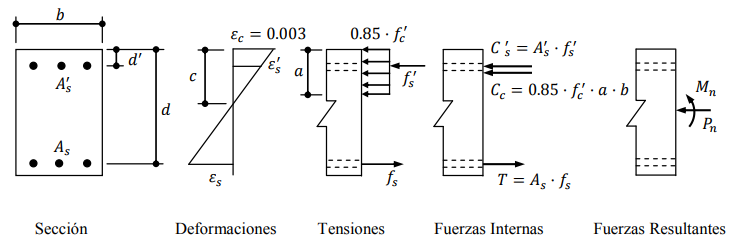
\includegraphics[scale=0.67]{IMAGENES/c1.PNG}
    \caption*{\small Fuente: \it \cite{cordova2015}}
    \label{vig}
\end{figure}
\newpage
\begin{figure}[ht!]
    \centering
    \caption{Diagrama de interacción en una columna}
    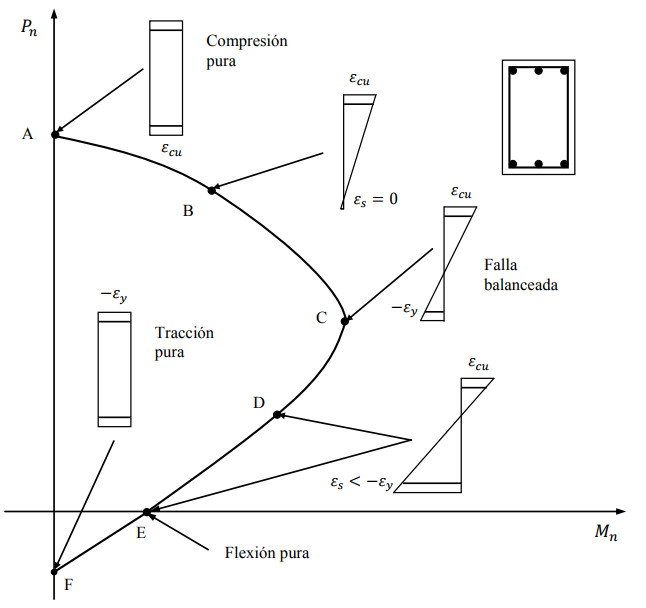
\includegraphics[scale=0.67]{IMAGENES/c2.PNG}
    \caption*{\small Fuente: \it \cite{cordova2015}}
    \label{vig}
\end{figure}
\noindent Preliminarmente se considerara $\nvc$ varillas de 5/8", lo cual cumple con la cuantía mínima del 1\%.\\
Capacidad máxima a carga axial de la columna.
\begin{align*}
\phi P_{n}=0,80 \cdot 0,70 \cdot\left[0,85 \cdot \fc \cdot\left(\Ag-\Ast\right)+\fy \cdot \Ast\right]=\pn \mathrm{~ton}
\end{align*}
\newpage
\begin{figure}[h!]
    \centering
    \subfigure[Eje débil]{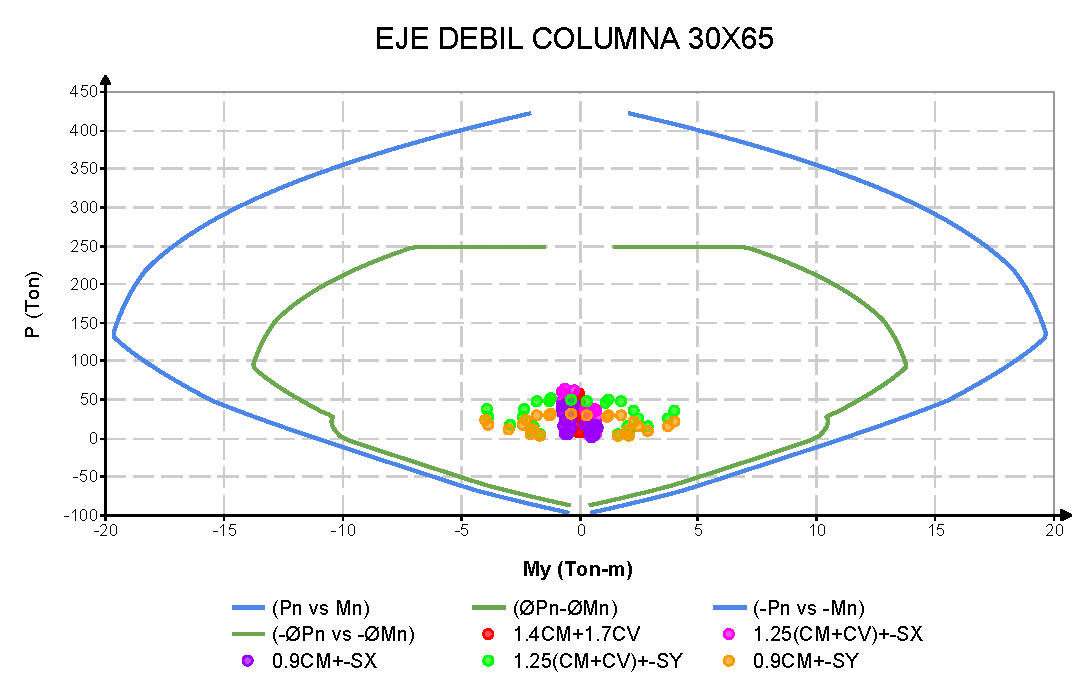
\includegraphics[width=150mm]{IMAGENES/colx.pdf}}\hspace{0mm}
    \subfigure[Eje fuerte]{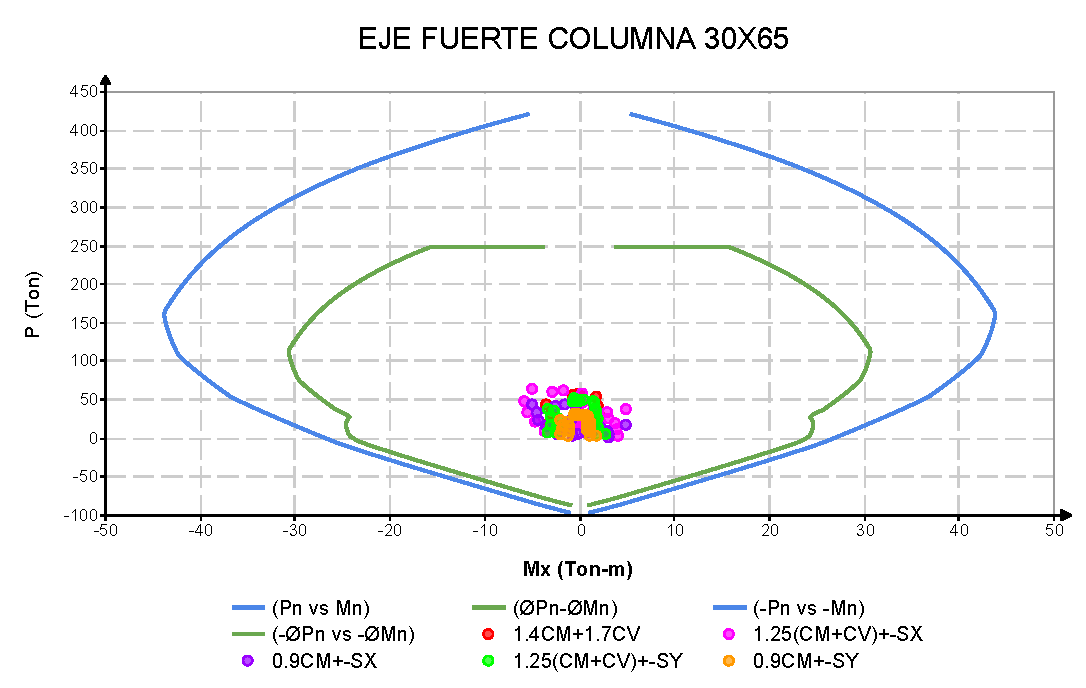
\includegraphics[width=150mm]{IMAGENES/coly.pdf}}
    \caption{Diagrama de interacción de la columna C-1 30x65 cm}
    \label{reqv}
\end{figure}

\begin{figure}[ht!]
    \centering
    \caption{Corte por capacidad en columnas}
    \subfigure[Fuerza cortante de columnas en sistemas de muros ]{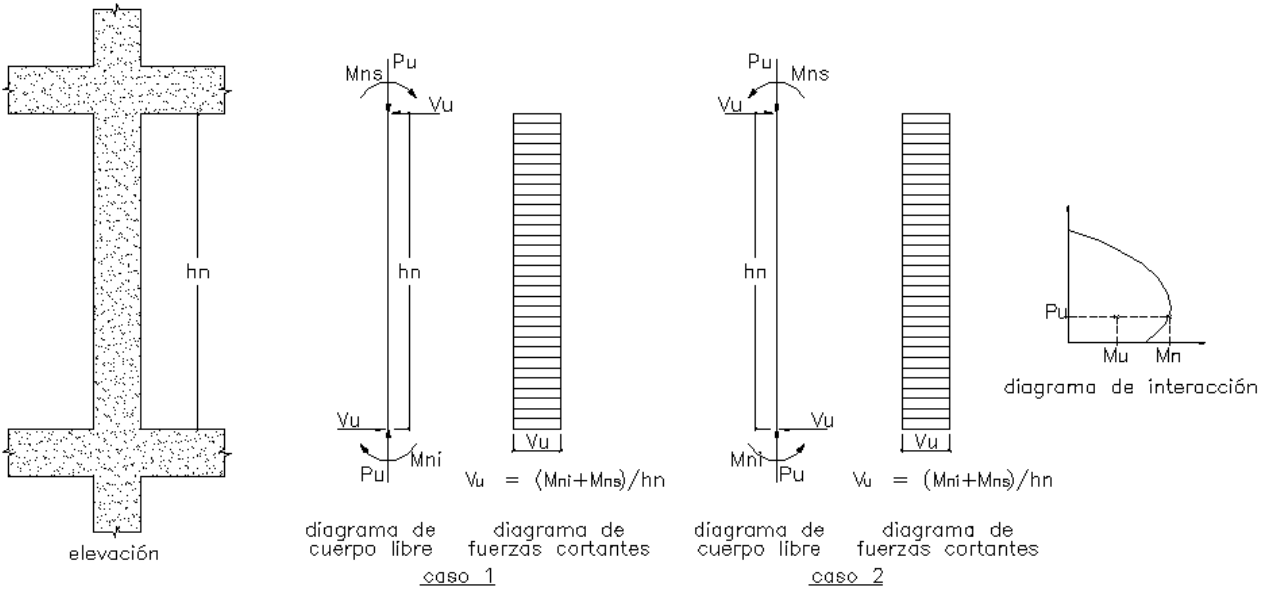
\includegraphics[width=150mm]{IMAGENES/colm.PNG}}\hspace{0mm}
    \subfigure[Fuerza cortante de columnas en sistemas duales o aporticados]{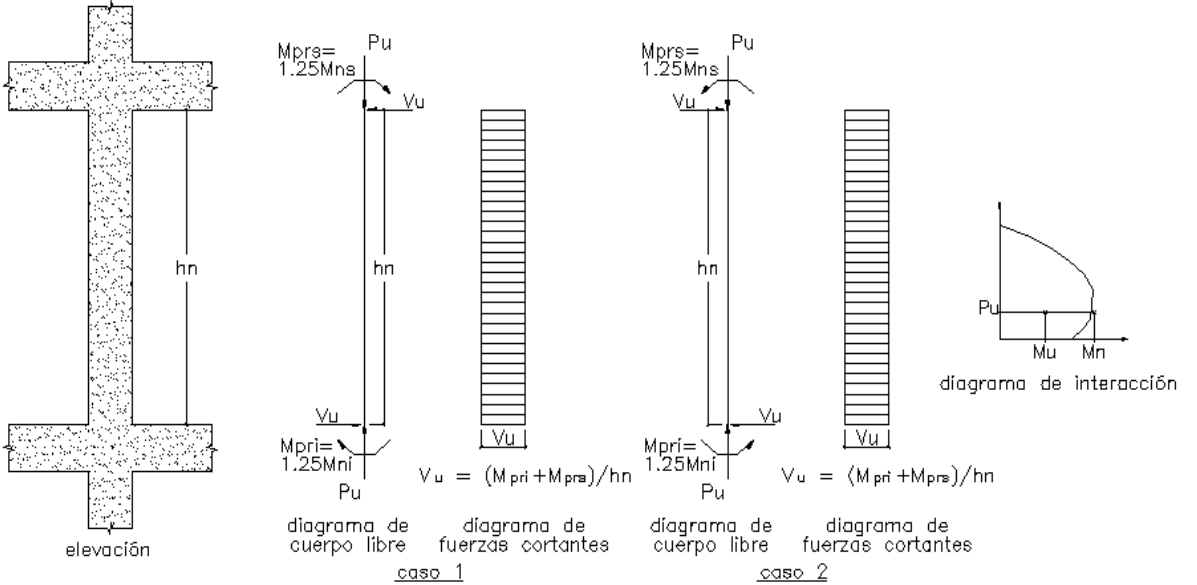
\includegraphics[width=150mm]{IMAGENES/colp.PNG}}
    \caption*{\small Fuente: \it \cite{E-060}}
    \label{reqv}
\end{figure}
\begin{align}
V_{u,1}=\frac{M_{n i}+M_{n s}}{h_{n}}\label{vcap1}\\
V_{u,2}=\frac{M_{p i}+M_{p s}}{h_{n}}\label{vcap2}
\end{align}
\newpage
\noindent
Donde:\\
$V_{u,1}$: Cortante en columnas, sistema de muros\\
$V_{u,2}$: Cortante en columnas, sistema de pórticos\\
$M_{n i}, M_{n s}$: Momentos nominales inferior e superior de la columna\\
$M_{p i}, M_{p s}$: Momentos probables inferior e superior de la columna\\

\subsubsection{Resistencia a corte Cap. 11}
La resistencia a cortante del concreto en una columna en compresión y tracción, esta dado respectivamente por:
\begin{flalign}
&\textup{Ecu.(11.4) E-060:}&\phi V_{c}&=\phi_{c} \cdot 0,53 \cdot \sqrt{f_{c}^{\prime}} \cdot b \cdot d \cdot\left(1+\frac{N_{u}}{140 \cdot A_{g}}\right)&&\label{vc1}\\
&\textup{Ecu.(11.8) E-060:}&\phi V_{c}&=\phi_{c} \cdot 0,53 \cdot \sqrt{f_{c}^{\prime}} \cdot b \cdot d \cdot\left(1-\frac{N_{u}}{35 \cdot A_{g}}\right)\label{vc2}
\end{flalign}
\noindent
Donde:\\
$N_{u}:$ Es la carga axial\\
$A_{g}:$ Es el área bruta de la sección\\
$d:$ Peralte efectivo en la dirección de análisis\\
$b:$ Ancho de la columna en la dirección de análisis\\
\noindent Los peraltes efectivos en las direcciones fuerte y débil de la columna serán:
\FPset\rec{4}
\FPeval{\dest}{round(3*2.54/8,2)}
\FPeval{\dvarc}{round(5*2.54/8,2)}
\FPeval{\defecx}{round(\hc-\rec-\dest-\dvarc/2,2)}
\FPeval{\defecy}{round(\bc-\rec-\dest-\dvarc/2,2)}
\FPeval{\vmaxx}{round(2.1*\rc*\hc*\defecx/1000,2)}
\FPeval{\vmaxy}{round(2.1*\rc*\bc*\defecy/1000,2)}
\begin{flalign*}
d_{x}=h_{c}-r_{e}-d_{e}-d_{b}/2&=\hc-\rec-\dest-\dvarc/2=\defecx \mathrm{~cm}\\
d_{y}=b_{c}-r_{e}-d_{e}-d_{b}/2&=\bc-\rec-\dest-\dvarc/2=\defecy \mathrm{~cm}
\end{flalign*}
\noindent La máxima capacidad de los estribos a corte en las direcciones fuerte y débil de la columna según la ecuación \ref{vmax} serán:
\begin{flalign*}
V_{ex, \max }&=2,1 \cdot \sqrt{\fc} \cdot \hc \cdot \defecx=\vmaxx \mathrm{ton}\\
V_{ey, \max }&=2,1 \cdot \sqrt{\fc} \cdot \bc \cdot \defecy=\vmaxy \mathrm{ton}
\end{flalign*}
\newpage
\begin{table}[ht!]
  \centering
  \caption{Diseño por capacidad en columnas (a)}
    {
\extrarowheight = 0ex
\renewcommand{\arraystretch}{1.2}
\begin{tabular}{*{2}{>{\centering\arraybackslash}m{0.8cm}}*{3}{|>{\centering\arraybackslash}m{1.5cm}}*{3}{|>{\centering\arraybackslash}m{1cm}}*{1}{|>{\centering\arraybackslash}m{1.1cm}}*{1}{|>{\centering\arraybackslash}m{1cm}}|}
\hline
\multicolumn{10}{|c|}{\textit{\textbf{1.25(CM+CV)+SX}}}                                                                                                                                                                                                          \\ \hline
\multicolumn{1}{|c|}{\multirow{2}{*}{\textbf{Piso}}} & \multicolumn{1}{c|}{(1)}            & \multicolumn{1}{c|}{(2)}               & \multicolumn{1}{c|}{(3)}            & \multicolumn{1}{c|}{(4)}                & \multicolumn{1}{c|}{(5)}                    & \multicolumn{1}{c|}{(6)}                    & \multicolumn{1}{c|}{(7)}                    & \multicolumn{1}{c|}{(8)}                & (9)                    \\ \cline{2-10} 
\multicolumn{1}{|c|}{}                               & \textbf{h (m)} & \textbf{Pu (ton)} & \textbf{a (cm)} & \textbf{Mn (ton.m)} & \textbf{Vu (ton)}     & \textbf{$\phi$Vc (ton)}    & \textbf{Ve}          & \textbf{ramas}    & \textbf{s (cm)}        \\ \hline
\multicolumn{1}{|c|}{\multirow{2}{*}{5}}             & \multicolumn{1}{c|}{2.2}            & \multicolumn{1}{c|}{-7.44}             & \multicolumn{1}{c|}{10.76}          & \multicolumn{1}{c|}{28.11}              & \multicolumn{1}{c|}{\multirow{2}{*}{25.67}} & \multicolumn{1}{c|}{\multirow{2}{*}{11.92}} & \multicolumn{1}{c|}{\multirow{2}{*}{16.17}} & \multicolumn{1}{c|}{\multirow{2}{*}{3}} & \multirow{2}{*}{32.89} \\ \cline{2-5}
\multicolumn{1}{|c|}{}                               & \multicolumn{1}{c|}{0}              & \multicolumn{1}{c|}{-8.73}             & \multicolumn{1}{c|}{10.89}          & \multicolumn{1}{c|}{28.37}              & \multicolumn{1}{c|}{}                       & \multicolumn{1}{c|}{}                       & \multicolumn{1}{c|}{}                       & \multicolumn{1}{c|}{}                   &                        \\ \hline
\multicolumn{1}{|c|}{\multirow{2}{*}{4}}             & \multicolumn{1}{c|}{2.2}            & \multicolumn{1}{c|}{-19.93}            & \multicolumn{1}{c|}{12.05}          & \multicolumn{1}{c|}{30.54}              & \multicolumn{1}{c|}{\multirow{2}{*}{27.88}} & \multicolumn{1}{c|}{\multirow{2}{*}{12.45}} & \multicolumn{1}{c|}{\multirow{2}{*}{18.14}} & \multicolumn{1}{c|}{\multirow{2}{*}{3}} & \multirow{2}{*}{29.32} \\ \cline{2-5}
\multicolumn{1}{|c|}{}                               & \multicolumn{1}{c|}{0}              & \multicolumn{1}{c|}{-21.22}            & \multicolumn{1}{c|}{12.19}          & \multicolumn{1}{c|}{30.79}              & \multicolumn{1}{c|}{}                       & \multicolumn{1}{c|}{}                       & \multicolumn{1}{c|}{}                       & \multicolumn{1}{c|}{}                   &                        \\ \hline
\multicolumn{1}{|c|}{\multirow{2}{*}{3}}             & \multicolumn{1}{c|}{2.2}            & \multicolumn{1}{c|}{-32.94}            & \multicolumn{1}{c|}{13.53}          & \multicolumn{1}{c|}{32.99}              & \multicolumn{1}{c|}{\multirow{2}{*}{30.11}} & \multicolumn{1}{c|}{\multirow{2}{*}{13.01}} & \multicolumn{1}{c|}{\multirow{2}{*}{20.12}} & \multicolumn{1}{c|}{\multirow{2}{*}{3}} & \multirow{2}{*}{26.44} \\ \cline{2-5}
\multicolumn{1}{|c|}{}                               & \multicolumn{1}{c|}{0}              & \multicolumn{1}{c|}{-34.23}            & \multicolumn{1}{c|}{13.69}          & \multicolumn{1}{c|}{33.24}              & \multicolumn{1}{c|}{}                       & \multicolumn{1}{c|}{}                       & \multicolumn{1}{c|}{}                       & \multicolumn{1}{c|}{}                   &                        \\ \hline
\multicolumn{1}{|c|}{\multirow{2}{*}{2}}             & \multicolumn{1}{c|}{2.2}            & \multicolumn{1}{c|}{-46.19}            & \multicolumn{1}{c|}{15.17}          & \multicolumn{1}{c|}{35.37}              & \multicolumn{1}{c|}{\multirow{2}{*}{32.26}} & \multicolumn{1}{c|}{\multirow{2}{*}{13.57}} & \multicolumn{1}{c|}{\multirow{2}{*}{21.99}} & \multicolumn{1}{c|}{\multirow{2}{*}{3}} & \multirow{2}{*}{24.19} \\ \cline{2-5}
\multicolumn{1}{|c|}{}                               & \multicolumn{1}{c|}{0}              & \multicolumn{1}{c|}{-47.47}            & \multicolumn{1}{c|}{15.34}          & \multicolumn{1}{c|}{35.60}              & \multicolumn{1}{c|}{}                       & \multicolumn{1}{c|}{}                       & \multicolumn{1}{c|}{}                       & \multicolumn{1}{c|}{}                   &                        \\ \hline
\multicolumn{1}{|c|}{\multirow{2}{*}{1}}             & \multicolumn{1}{c|}{2.8}            & \multicolumn{1}{c|}{-59.25}            & \multicolumn{1}{c|}{16.78}          & \multicolumn{1}{c|}{37.33}              & \multicolumn{1}{c|}{\multirow{2}{*}{26.73}} & \multicolumn{1}{c|}{\multirow{2}{*}{14.12}} & \multicolumn{1}{c|}{\multirow{2}{*}{14.83}} & \multicolumn{1}{c|}{\multirow{2}{*}{3}} & \multirow{2}{*}{35.86} \\ \cline{2-5}
\multicolumn{1}{|c|}{}                               & \multicolumn{1}{c|}{0}              & \multicolumn{1}{c|}{-60.88}            & \multicolumn{1}{c|}{16.96}          & \multicolumn{1}{c|}{37.52}              & \multicolumn{1}{c|}{}                       & \multicolumn{1}{c|}{}                       & \multicolumn{1}{c|}{}                       & \multicolumn{1}{c|}{}                   &                        \\ \hline
\multicolumn{1}{|c|}{\multirow{2}{*}{0}}             & \multicolumn{1}{c|}{2.15}           & \multicolumn{1}{c|}{-62.91}            & \multicolumn{1}{c|}{17.19}          & \multicolumn{1}{c|}{37.75}              & \multicolumn{1}{c|}{\multirow{2}{*}{35.18}} & \multicolumn{1}{c|}{\multirow{2}{*}{14.28}} & \multicolumn{1}{c|}{\multirow{2}{*}{24.59}} & \multicolumn{1}{c|}{\multirow{2}{*}{3}} & \multirow{2}{*}{21.64} \\ \cline{2-5}
\multicolumn{1}{|c|}{}                               & \multicolumn{1}{c|}{0}              & \multicolumn{1}{c|}{-64.17}            & \multicolumn{1}{c|}{17.33}          & \multicolumn{1}{c|}{37.89}              & \multicolumn{1}{c|}{}                       & \multicolumn{1}{c|}{}                       & \multicolumn{1}{c|}{}                       & \multicolumn{1}{c|}{}                   &                        \\ \hline
\end{tabular}
}
\end{table}
\vspace{0.5cm}
% Please add the following required packages to your document preamble:
% \usepackage{multirow}
\begin{table}[hb!]
  \centering
  \caption{Diseño por capacidad en columnas (b)}
    {
\extrarowheight = 0ex
\renewcommand{\arraystretch}{1.2}
\begin{tabular}{*{2}{>{\centering\arraybackslash}m{0.8cm}}*{3}{|>{\centering\arraybackslash}m{1.5cm}}*{3}{|>{\centering\arraybackslash}m{1cm}}*{1}{|>{\centering\arraybackslash}m{1.1cm}}*{1}{|>{\centering\arraybackslash}m{1cm}}|}
\hline
\multicolumn{10}{|c|}{\textit{\textbf{1.25(CM+CV)-SX}}}                                                                                                                                                                                                          \\ \hline
\multicolumn{1}{|c|}{\multirow{2}{*}{\textbf{Piso}}} & \multicolumn{1}{c|}{(1)}            & \multicolumn{1}{c|}{(2)}               & \multicolumn{1}{c|}{(3)}            & \multicolumn{1}{c|}{(4)}                & \multicolumn{1}{c|}{(5)}                    & \multicolumn{1}{c|}{(6)}                    & \multicolumn{1}{c|}{(7)}                    & \multicolumn{1}{c|}{(8)}                & (9)                    \\ \cline{2-10} 
\multicolumn{1}{|c|}{}                               & \textbf{h (m)} & \textbf{Pu (ton)} & \textbf{a (cm)} & \textbf{Mn (ton.m)} & \textbf{Vu (ton)}     & \textbf{$\phi$Vc (ton)}    & \textbf{Ve}          & \textbf{ramas}    & \textbf{s (cm)}        \\ \hline
\multicolumn{1}{|c|}{\multirow{2}{*}{5}}             & \multicolumn{1}{c|}{2.2}            & \multicolumn{1}{c|}{-4.22}             & \multicolumn{1}{c|}{10.45}           & \multicolumn{1}{c|}{27.47}               & \multicolumn{1}{c|}{\multirow{2}{*}{25.10}} & \multicolumn{1}{c|}{\multirow{2}{*}{11.78}} & \multicolumn{1}{c|}{\multirow{2}{*}{15.66}} & \multicolumn{1}{c|}{\multirow{2}{*}{3}} & \multirow{2}{*}{33.97} \\ \cline{2-5}
\multicolumn{1}{|c|}{}                               & \multicolumn{1}{c|}{0}              & \multicolumn{1}{c|}{-5.51}             & \multicolumn{1}{c|}{10.58}           & \multicolumn{1}{c|}{27.74}               & \multicolumn{1}{c|}{}                       & \multicolumn{1}{c|}{}                       & \multicolumn{1}{c|}{}                       & \multicolumn{1}{c|}{}                   &                        \\ \hline
\multicolumn{1}{|c|}{\multirow{2}{*}{4}}             & \multicolumn{1}{c|}{2.2}            & \multicolumn{1}{c|}{-11.91}            & \multicolumn{1}{c|}{11.21}           & \multicolumn{1}{c|}{28.99}               & \multicolumn{1}{c|}{\multirow{2}{*}{26.47}} & \multicolumn{1}{c|}{\multirow{2}{*}{12.11}} & \multicolumn{1}{c|}{\multirow{2}{*}{16.89}} & \multicolumn{1}{c|}{\multirow{2}{*}{3}} & \multirow{2}{*}{31.50} \\ \cline{2-5}
\multicolumn{1}{|c|}{}                               & \multicolumn{1}{c|}{0}              & \multicolumn{1}{c|}{-13.20}            & \multicolumn{1}{c|}{11.34}           & \multicolumn{1}{c|}{29.24}               & \multicolumn{1}{c|}{}                       & \multicolumn{1}{c|}{}                       & \multicolumn{1}{c|}{}                       & \multicolumn{1}{c|}{}                   &                        \\ \hline
\multicolumn{1}{|c|}{\multirow{2}{*}{3}}             & \multicolumn{1}{c|}{2.2}            & \multicolumn{1}{c|}{-19.16}            & \multicolumn{1}{c|}{11.97}           & \multicolumn{1}{c|}{30.40}               & \multicolumn{1}{c|}{\multirow{2}{*}{27.75}} & \multicolumn{1}{c|}{\multirow{2}{*}{12.42}} & \multicolumn{1}{c|}{\multirow{2}{*}{18.03}} & \multicolumn{1}{c|}{\multirow{2}{*}{3}} & \multirow{2}{*}{29.50} \\ \cline{2-5}
\multicolumn{1}{|c|}{}                               & \multicolumn{1}{c|}{0}              & \multicolumn{1}{c|}{-20.45}            & \multicolumn{1}{c|}{12.11}           & \multicolumn{1}{c|}{30.65}               & \multicolumn{1}{c|}{}                       & \multicolumn{1}{c|}{}                       & \multicolumn{1}{c|}{}                       & \multicolumn{1}{c|}{}                   &                        \\ \hline
\multicolumn{1}{|c|}{\multirow{2}{*}{2}}             & \multicolumn{1}{c|}{2.2}            & \multicolumn{1}{c|}{-26.38}            & \multicolumn{1}{c|}{12.77}           & \multicolumn{1}{c|}{31.77}               & \multicolumn{1}{c|}{\multirow{2}{*}{29.00}} & \multicolumn{1}{c|}{\multirow{2}{*}{12.73}} & \multicolumn{1}{c|}{\multirow{2}{*}{19.14}} & \multicolumn{1}{c|}{\multirow{2}{*}{3}} & \multirow{2}{*}{27.79} \\ \cline{2-5}
\multicolumn{1}{|c|}{}                               & \multicolumn{1}{c|}{0}              & \multicolumn{1}{c|}{-27.67}            & \multicolumn{1}{c|}{12.92}           & \multicolumn{1}{c|}{32.02}               & \multicolumn{1}{c|}{}                       & \multicolumn{1}{c|}{}                       & \multicolumn{1}{c|}{}                       & \multicolumn{1}{c|}{}                   &                        \\ \hline
\multicolumn{1}{|c|}{\multirow{2}{*}{1}}             & \multicolumn{1}{c|}{2.8}            & \multicolumn{1}{c|}{-34.02}          & \multicolumn{1}{c|}{13.66}           & \multicolumn{1}{c|}{33.19}           & \multicolumn{1}{c|}{\multirow{2}{*}{23.82}} & \multicolumn{1}{c|}{\multirow{2}{*}{13.05}} & \multicolumn{1}{c|}{\multirow{2}{*}{12.67}} & \multicolumn{1}{c|}{\multirow{2}{*}{3}} & \multirow{2}{*}{42.00} \\ \cline{2-5}
\multicolumn{1}{|c|}{}                               & \multicolumn{1}{c|}{0}              & \multicolumn{1}{c|}{-35.66}          & \multicolumn{1}{c|}{13.86}           & \multicolumn{1}{c|}{33.50}           & \multicolumn{1}{c|}{}                       & \multicolumn{1}{c|}{}                       & \multicolumn{1}{c|}{}                       & \multicolumn{1}{c|}{}                   &                        \\ \hline
\multicolumn{1}{|c|}{\multirow{2}{*}{0}}             & \multicolumn{1}{c|}{2.15}           & \multicolumn{1}{c|}{-35.97}            & \multicolumn{1}{c|}{13.90}           & \multicolumn{1}{c|}{33.56}               & \multicolumn{1}{c|}{\multirow{2}{*}{31.32}} & \multicolumn{1}{c|}{\multirow{2}{*}{13.13}} & \multicolumn{1}{c|}{\multirow{2}{*}{21.40}} & \multicolumn{1}{c|}{\multirow{2}{*}{3}} & \multirow{2}{*}{24.86} \\ \cline{2-5}
\multicolumn{1}{|c|}{}                               & \multicolumn{1}{c|}{0}              & \multicolumn{1}{c|}{-37.23}            & \multicolumn{1}{c|}{14.05}           & \multicolumn{1}{c|}{33.78}               & \multicolumn{1}{c|}{}                       & \multicolumn{1}{c|}{}                       & \multicolumn{1}{c|}{}                       & \multicolumn{1}{c|}{}                   &                        \\ \hline
\end{tabular}
}
\end{table}
\begin{table}[ht!]
  \centering
  \caption{Diseño por capacidad en columnas (c)}
    {
\extrarowheight = 0ex
\renewcommand{\arraystretch}{1.2}
\begin{tabular}{*{2}{>{\centering\arraybackslash}m{0.8cm}}*{3}{|>{\centering\arraybackslash}m{1.5cm}}*{3}{|>{\centering\arraybackslash}m{1cm}}*{1}{|>{\centering\arraybackslash}m{1.1cm}}*{1}{|>{\centering\arraybackslash}m{1cm}}|}
\hline
\multicolumn{10}{|c|}{\textit{\textbf{0.9CM+SX}}}                                                                                                                                                                                                          \\ \hline
\multicolumn{1}{|c|}{\multirow{2}{*}{\textbf{Piso}}} & \multicolumn{1}{c|}{(1)}            & \multicolumn{1}{c|}{(2)}               & \multicolumn{1}{c|}{(3)}            & \multicolumn{1}{c|}{(4)}                & \multicolumn{1}{c|}{(5)}                    & \multicolumn{1}{c|}{(6)}                    & \multicolumn{1}{c|}{(7)}                    & \multicolumn{1}{c|}{(8)}                & (9)                    \\ \cline{2-10} 
\multicolumn{1}{|c|}{}                               & \textbf{h (m)} & \textbf{Pu (ton)} & \textbf{a (cm)} & \textbf{Mn (ton.m)} & \textbf{Vu (Ton)}     & \textbf{$\phi$Vc (ton)}    & \textbf{Ve}          & \textbf{ramas}    & \textbf{s (cm)}        \\ \hline
\multicolumn{1}{|c|}{\multirow{2}{*}{5}}             & \multicolumn{1}{c|}{2.2}            & \multicolumn{1}{c|}{-5.30}             & \multicolumn{1}{c|}{10.56}          & \multicolumn{1}{c|}{27.70}              & \multicolumn{1}{c|}{\multirow{2}{*}{25.26}} & \multicolumn{1}{c|}{\multirow{2}{*}{11.83}} & \multicolumn{1}{c|}{\multirow{2}{*}{15.80}} & \multicolumn{1}{c|}{\multirow{2}{*}{3}} & \multirow{2}{*}{33.66} \\ \cline{2-5}
\multicolumn{1}{|c|}{}                               & \multicolumn{1}{c|}{0}              & \multicolumn{1}{c|}{-6.23}             & \multicolumn{1}{c|}{10.65}          & \multicolumn{1}{c|}{27.88}              & \multicolumn{1}{c|}{}                       & \multicolumn{1}{c|}{}                       & \multicolumn{1}{c|}{}                       & \multicolumn{1}{c|}{}                   &                        \\ \hline
\multicolumn{1}{|c|}{\multirow{2}{*}{4}}             & \multicolumn{1}{c|}{2.2}            & \multicolumn{1}{c|}{-13.87}            & \multicolumn{1}{c|}{11.41}          & \multicolumn{1}{c|}{29.37}              & \multicolumn{1}{c|}{\multirow{2}{*}{26.79}} & \multicolumn{1}{c|}{\multirow{2}{*}{12.19}} & \multicolumn{1}{c|}{\multirow{2}{*}{17.17}} & \multicolumn{1}{c|}{\multirow{2}{*}{3}} & \multirow{2}{*}{30.99} \\ \cline{2-5}
\multicolumn{1}{|c|}{}                               & \multicolumn{1}{c|}{0}              & \multicolumn{1}{c|}{-14.80}            & \multicolumn{1}{c|}{11.51}          & \multicolumn{1}{c|}{29.56}              & \multicolumn{1}{c|}{}                       & \multicolumn{1}{c|}{}                       & \multicolumn{1}{c|}{}                       & \multicolumn{1}{c|}{}                   &                        \\ \hline
\multicolumn{1}{|c|}{\multirow{2}{*}{3}}             & \multicolumn{1}{c|}{2.2}            & \multicolumn{1}{c|}{-22.95}            & \multicolumn{1}{c|}{12.39}          & \multicolumn{1}{c|}{31.13}              & \multicolumn{1}{c|}{\multirow{2}{*}{28.38}} & \multicolumn{1}{c|}{\multirow{2}{*}{12.58}} & \multicolumn{1}{c|}{\multirow{2}{*}{18.59}} & \multicolumn{1}{c|}{\multirow{2}{*}{3}} & \multirow{2}{*}{28.62} \\ \cline{2-5}
\multicolumn{1}{|c|}{}                               & \multicolumn{1}{c|}{0}              & \multicolumn{1}{c|}{-23.88}            & \multicolumn{1}{c|}{12.49}          & \multicolumn{1}{c|}{31.30}              & \multicolumn{1}{c|}{}                       & \multicolumn{1}{c|}{}                       & \multicolumn{1}{c|}{}                       & \multicolumn{1}{c|}{}                   &                        \\ \hline
\multicolumn{1}{|c|}{\multirow{2}{*}{2}}             & \multicolumn{1}{c|}{2.2}            & \multicolumn{1}{c|}{-32.22}            & \multicolumn{1}{c|}{13.45}          & \multicolumn{1}{c|}{32.87}              & \multicolumn{1}{c|}{\multirow{2}{*}{29.96}} & \multicolumn{1}{c|}{\multirow{2}{*}{12.97}} & \multicolumn{1}{c|}{\multirow{2}{*}{19.98}} & \multicolumn{1}{c|}{\multirow{2}{*}{3}} & \multirow{2}{*}{26.63} \\ \cline{2-5}
\multicolumn{1}{|c|}{}                               & \multicolumn{1}{c|}{0}              & \multicolumn{1}{c|}{-33.15}            & \multicolumn{1}{c|}{13.56}          & \multicolumn{1}{c|}{33.04}              & \multicolumn{1}{c|}{}                       & \multicolumn{1}{c|}{}                       & \multicolumn{1}{c|}{}                       & \multicolumn{1}{c|}{}                   &                        \\ \hline
\multicolumn{1}{|c|}{\multirow{2}{*}{1}}             & \multicolumn{1}{c|}{2.8}            & \multicolumn{1}{c|}{-41.27}            & \multicolumn{1}{c|}{14.55}          & \multicolumn{1}{c|}{34.51}              & \multicolumn{1}{c|}{\multirow{2}{*}{24.73}} & \multicolumn{1}{c|}{\multirow{2}{*}{13.36}} & \multicolumn{1}{c|}{\multirow{2}{*}{13.37}} & \multicolumn{1}{c|}{\multirow{2}{*}{3}} & \multirow{2}{*}{39.78} \\ \cline{2-5}
\multicolumn{1}{|c|}{}                               & \multicolumn{1}{c|}{0}              & \multicolumn{1}{c|}{-42.45}            & \multicolumn{1}{c|}{14.70}          & \multicolumn{1}{c|}{34.72}              & \multicolumn{1}{c|}{}                       & \multicolumn{1}{c|}{}                       & \multicolumn{1}{c|}{}                       & \multicolumn{1}{c|}{}                   &                        \\ \hline
\multicolumn{1}{|c|}{\multirow{2}{*}{0}}             & \multicolumn{1}{c|}{2.15}           & \multicolumn{1}{c|}{-44.17}            & \multicolumn{1}{c|}{14.92}          & \multicolumn{1}{c|}{35.03}              & \multicolumn{1}{c|}{\multirow{2}{*}{32.66}} & \multicolumn{1}{c|}{\multirow{2}{*}{13.48}} & \multicolumn{1}{c|}{\multirow{2}{*}{22.56}} & \multicolumn{1}{c|}{\multirow{2}{*}{3}} & \multirow{2}{*}{23.58} \\ \cline{2-5}
\multicolumn{1}{|c|}{}                               & \multicolumn{1}{c|}{0}              & \multicolumn{1}{c|}{-45.08}            & \multicolumn{1}{c|}{15.03}          & \multicolumn{1}{c|}{35.18}              & \multicolumn{1}{c|}{}                       & \multicolumn{1}{c|}{}                       & \multicolumn{1}{c|}{}                       & \multicolumn{1}{c|}{}                   &                        \\ \hline
\end{tabular}
}
\end{table}
%\vspace{0.5cm}
% Please add the following required packages to your document preamble:
% \usepackage{multirow}
\begin{table}[hb!]
  \centering
  \caption{Diseño por capacidad en columnas (d)}
    {
\extrarowheight = 0ex
\renewcommand{\arraystretch}{1.2}
\begin{tabular}{*{2}{>{\centering\arraybackslash}m{0.8cm}}*{3}{|>{\centering\arraybackslash}m{1.5cm}}*{3}{|>{\centering\arraybackslash}m{1cm}}*{1}{|>{\centering\arraybackslash}m{1.1cm}}*{1}{|>{\centering\arraybackslash}m{1cm}}|}
\hline
\multicolumn{10}{|c|}{\textit{\textbf{0.9CM-SX}}}                                                                                                                                                                                                          \\ \hline
\multicolumn{1}{|c|}{\multirow{2}{*}{\textbf{Piso}}} & \multicolumn{1}{c|}{(1)}            & \multicolumn{1}{c|}{(2)}               & \multicolumn{1}{c|}{(3)}            & \multicolumn{1}{c|}{(4)}                & \multicolumn{1}{c|}{(5)}                    & \multicolumn{1}{c|}{(6)}                    & \multicolumn{1}{c|}{(7)}                    & \multicolumn{1}{c|}{(8)}                & (9)                    \\ \cline{2-10} 
\multicolumn{1}{|c|}{}                               & \textbf{h (m)} & \textbf{Pu (ton)} & \textbf{a (cm)} & \textbf{Mn (ton.m)} & \textbf{Vu (Ton)}     & \textbf{$\phi$Vc (ton)}    & \textbf{Ve}          & \textbf{ramas}    & \textbf{s (cm)}        \\ \hline
\multicolumn{1}{|c|}{\multirow{2}{*}{5}}             & \multicolumn{1}{c|}{2.2}            & \multicolumn{1}{c|}{-2.08}             & \multicolumn{1}{c|}{10.25}          & \multicolumn{1}{c|}{27.05}              & \multicolumn{1}{c|}{\multirow{2}{*}{24.68}} & \multicolumn{1}{c|}{\multirow{2}{*}{11.69}} & \multicolumn{1}{c|}{\multirow{2}{*}{15.28}} & \multicolumn{1}{c|}{\multirow{2}{*}{3}} & \multirow{2}{*}{34.83} \\ \cline{2-5}
\multicolumn{1}{|c|}{}                               & \multicolumn{1}{c|}{0}              & \multicolumn{1}{c|}{-3.01}             & \multicolumn{1}{c|}{10.34}          & \multicolumn{1}{c|}{27.24}              & \multicolumn{1}{c|}{}                       & \multicolumn{1}{c|}{}                       & \multicolumn{1}{c|}{}                       & \multicolumn{1}{c|}{}                   &                        \\ \hline
\multicolumn{1}{|c|}{\multirow{2}{*}{4}}             & \multicolumn{1}{c|}{2.2}            & \multicolumn{1}{c|}{-5.86}             & \multicolumn{1}{c|}{10.61}          & \multicolumn{1}{c|}{27.80}              & \multicolumn{1}{c|}{\multirow{2}{*}{25.36}} & \multicolumn{1}{c|}{\multirow{2}{*}{11.85}} & \multicolumn{1}{c|}{\multirow{2}{*}{15.89}} & \multicolumn{1}{c|}{\multirow{2}{*}{3}} & \multirow{2}{*}{33.49} \\ \cline{2-5}
\multicolumn{1}{|c|}{}                               & \multicolumn{1}{c|}{0}              & \multicolumn{1}{c|}{-6.78}             & \multicolumn{1}{c|}{10.70}          & \multicolumn{1}{c|}{27.98}              & \multicolumn{1}{c|}{}                       & \multicolumn{1}{c|}{}                       & \multicolumn{1}{c|}{}                       & \multicolumn{1}{c|}{}                   &                        \\ \hline
\multicolumn{1}{|c|}{\multirow{2}{*}{3}}             & \multicolumn{1}{c|}{2.2}            & \multicolumn{1}{c|}{-9.17}             & \multicolumn{1}{c|}{10.93}          & \multicolumn{1}{c|}{28.44}              & \multicolumn{1}{c|}{\multirow{2}{*}{25.95}} & \multicolumn{1}{c|}{\multirow{2}{*}{11.99}} & \multicolumn{1}{c|}{\multirow{2}{*}{16.42}} & \multicolumn{1}{c|}{\multirow{2}{*}{3}} & \multirow{2}{*}{32.41} \\ \cline{2-5}
\multicolumn{1}{|c|}{}                               & \multicolumn{1}{c|}{0}              & \multicolumn{1}{c|}{-10.10}            & \multicolumn{1}{c|}{11.03}          & \multicolumn{1}{c|}{28.64}              & \multicolumn{1}{c|}{}                       & \multicolumn{1}{c|}{}                       & \multicolumn{1}{c|}{}                       & \multicolumn{1}{c|}{}                   &                        \\ \hline
\multicolumn{1}{|c|}{\multirow{2}{*}{2}}             & \multicolumn{1}{c|}{2.2}            & \multicolumn{1}{c|}{-12.42}            & \multicolumn{1}{c|}{11.26}          & \multicolumn{1}{c|}{29.09}              & \multicolumn{1}{c|}{\multirow{2}{*}{26.53}} & \multicolumn{1}{c|}{\multirow{2}{*}{12.13}} & \multicolumn{1}{c|}{\multirow{2}{*}{16.94}} & \multicolumn{1}{c|}{\multirow{2}{*}{3}} & \multirow{2}{*}{31.41} \\ \cline{2-5}
\multicolumn{1}{|c|}{}                               & \multicolumn{1}{c|}{0}              & \multicolumn{1}{c|}{-13.34}            & \multicolumn{1}{c|}{11.36}          & \multicolumn{1}{c|}{29.28}              & \multicolumn{1}{c|}{}                       & \multicolumn{1}{c|}{}                       & \multicolumn{1}{c|}{}                       & \multicolumn{1}{c|}{}                   &                        \\ \hline
\multicolumn{1}{|c|}{\multirow{2}{*}{1}}             & \multicolumn{1}{c|}{2.8}            & \multicolumn{1}{c|}{-16.05}            & \multicolumn{1}{c|}{11.64}          & \multicolumn{1}{c|}{29.80}              & \multicolumn{1}{c|}{\multirow{2}{*}{21.36}} & \multicolumn{1}{c|}{\multirow{2}{*}{12.29}} & \multicolumn{1}{c|}{\multirow{2}{*}{10.68}} & \multicolumn{1}{c|}{\multirow{2}{*}{3}} & \multirow{2}{*}{49.82} \\ \cline{2-5}
\multicolumn{1}{|c|}{}                               & \multicolumn{1}{c|}{0}              & \multicolumn{1}{c|}{-17.23}            & \multicolumn{1}{c|}{11.76}          & \multicolumn{1}{c|}{30.02}              & \multicolumn{1}{c|}{}                       & \multicolumn{1}{c|}{}                       & \multicolumn{1}{c|}{}                       & \multicolumn{1}{c|}{}                   &                        \\ \hline
\multicolumn{1}{|c|}{\multirow{2}{*}{0}}             & \multicolumn{1}{c|}{2.15}           & \multicolumn{1}{c|}{-17.23}            & \multicolumn{1}{c|}{11.76}          & \multicolumn{1}{c|}{30.02}              & \multicolumn{1}{c|}{\multirow{2}{*}{28.01}} & \multicolumn{1}{c|}{\multirow{2}{*}{12.34}} & \multicolumn{1}{c|}{\multirow{2}{*}{18.44}} & \multicolumn{1}{c|}{\multirow{2}{*}{3}} & \multirow{2}{*}{28.85} \\ \cline{2-5}
\multicolumn{1}{|c|}{}                               & \multicolumn{1}{c|}{0}              & \multicolumn{1}{c|}{-18.13}            & \multicolumn{1}{c|}{11.86}          & \multicolumn{1}{c|}{30.20}              & \multicolumn{1}{c|}{}                       & \multicolumn{1}{c|}{}                       & \multicolumn{1}{c|}{}                       & \multicolumn{1}{c|}{}                   &                        \\ \hline
\end{tabular}
}
\end{table}
\begin{table}[ht!]
  \centering
  \caption{Diseño por capacidad en columnas (e)}
    {
\extrarowheight = 0ex
\renewcommand{\arraystretch}{1.2}
\begin{tabular}{*{2}{>{\centering\arraybackslash}m{0.8cm}}*{3}{|>{\centering\arraybackslash}m{1.5cm}}*{3}{|>{\centering\arraybackslash}m{1cm}}*{1}{|>{\centering\arraybackslash}m{1.1cm}}*{1}{|>{\centering\arraybackslash}m{1cm}}|}
\hline
\multicolumn{10}{|c|}{\textit{\textbf{1.25(CM+CV)+SY}}}                                                                                                                                                                                                          \\ \hline
\multicolumn{1}{|c|}{\multirow{2}{*}{\textbf{Piso}}} & \multicolumn{1}{c|}{(1)}            & \multicolumn{1}{c|}{(2)}               & \multicolumn{1}{c|}{(3)}            & \multicolumn{1}{c|}{(4)}                & \multicolumn{1}{c|}{(5)}                    & \multicolumn{1}{c|}{(6)}                    & \multicolumn{1}{c|}{(7)}                    & \multicolumn{1}{c|}{(8)}                & (9)                    \\ \cline{2-10} 
\multicolumn{1}{|c|}{}                               & \textbf{h (m)} & \textbf{Pu (ton)} & \textbf{a (cm)} & \textbf{Mn (ton.m)} & \textbf{Vu (Ton)}     & \textbf{$\phi$Vc (ton)}    & \textbf{Ve}          & \textbf{ramas}    & \textbf{s (cm)}        \\ \hline
\multicolumn{1}{|c|}{\multirow{2}{*}{5}}             & \multicolumn{1}{c|}{2.2}            & \multicolumn{1}{c|}{-6.23}             & \multicolumn{1}{c|}{5.20}           & \multicolumn{1}{c|}{11.66}              & \multicolumn{1}{c|}{\multirow{2}{*}{13.31}} & \multicolumn{1}{c|}{\multirow{2}{*}{10.53}} & \multicolumn{1}{c|}{\multirow{2}{*}{3.28}} & \multicolumn{1}{c|}{\multirow{2}{*}{2}} & \multirow{2}{*}{44.31} \\ \cline{2-5}
\multicolumn{1}{|c|}{}                               & \multicolumn{1}{c|}{0}              & \multicolumn{1}{c|}{-7.51}             & \multicolumn{1}{c|}{5.25}           & \multicolumn{1}{c|}{11.77}              & \multicolumn{1}{c|}{}                       & \multicolumn{1}{c|}{}                       & \multicolumn{1}{c|}{}                      & \multicolumn{1}{c|}{}                   &                        \\ \hline
\multicolumn{1}{|c|}{\multirow{2}{*}{4}}             & \multicolumn{1}{c|}{2.2}            & \multicolumn{1}{c|}{-16.69}            & \multicolumn{1}{c|}{5.68}           & \multicolumn{1}{c|}{12.63}              & \multicolumn{1}{c|}{\multirow{2}{*}{14.43}} & \multicolumn{1}{c|}{\multirow{2}{*}{10.92}} & \multicolumn{1}{c|}{\multirow{2}{*}{4.13}} & \multicolumn{1}{c|}{\multirow{2}{*}{2}} & \multirow{2}{*}{35.19} \\ \cline{2-5}
\multicolumn{1}{|c|}{}                               & \multicolumn{1}{c|}{0}              & \multicolumn{1}{c|}{-17.98}            & \multicolumn{1}{c|}{5.75}           & \multicolumn{1}{c|}{12.76}              & \multicolumn{1}{c|}{}                       & \multicolumn{1}{c|}{}                       & \multicolumn{1}{c|}{}                      & \multicolumn{1}{c|}{}                   &                        \\ \hline
\multicolumn{1}{|c|}{\multirow{2}{*}{3}}             & \multicolumn{1}{c|}{2.2}            & \multicolumn{1}{c|}{-26.99}            & \multicolumn{1}{c|}{6.20}           & \multicolumn{1}{c|}{13.57}              & \multicolumn{1}{c|}{\multirow{2}{*}{15.49}} & \multicolumn{1}{c|}{\multirow{2}{*}{11.31}} & \multicolumn{1}{c|}{\multirow{2}{*}{4.92}} & \multicolumn{1}{c|}{\multirow{2}{*}{2}} & \multirow{2}{*}{29.50} \\ \cline{2-5}
\multicolumn{1}{|c|}{}                               & \multicolumn{1}{c|}{0}              & \multicolumn{1}{c|}{-28.27}            & \multicolumn{1}{c|}{6.27}           & \multicolumn{1}{c|}{13.69}              & \multicolumn{1}{c|}{}                       & \multicolumn{1}{c|}{}                       & \multicolumn{1}{c|}{}                      & \multicolumn{1}{c|}{}                   &                        \\ \hline
\multicolumn{1}{|c|}{\multirow{2}{*}{2}}             & \multicolumn{1}{c|}{2.2}            & \multicolumn{1}{c|}{-37.29}            & \multicolumn{1}{c|}{6.76}           & \multicolumn{1}{c|}{14.48}              & \multicolumn{1}{c|}{\multirow{2}{*}{16.52}} & \multicolumn{1}{c|}{\multirow{2}{*}{11.70}} & \multicolumn{1}{c|}{\multirow{2}{*}{5.67}} & \multicolumn{1}{c|}{\multirow{2}{*}{2}} & \multirow{2}{*}{25.58} \\ \cline{2-5}
\multicolumn{1}{|c|}{}                               & \multicolumn{1}{c|}{0}              & \multicolumn{1}{c|}{-38.58}            & \multicolumn{1}{c|}{6.83}           & \multicolumn{1}{c|}{14.59}              & \multicolumn{1}{c|}{}                       & \multicolumn{1}{c|}{}                       & \multicolumn{1}{c|}{}                      & \multicolumn{1}{c|}{}                   &                        \\ \hline
\multicolumn{1}{|c|}{\multirow{2}{*}{1}}             & \multicolumn{1}{c|}{2.8}            & \multicolumn{1}{c|}{-47.51}            & \multicolumn{1}{c|}{7.34}           & \multicolumn{1}{c|}{15.33}              & \multicolumn{1}{c|}{\multirow{2}{*}{13.75}} & \multicolumn{1}{c|}{\multirow{2}{*}{12.08}} & \multicolumn{1}{c|}{\multirow{2}{*}{1.96}} & \multicolumn{1}{c|}{\multirow{2}{*}{2}} & \multirow{2}{*}{73.92} \\ \cline{2-5}
\multicolumn{1}{|c|}{}                               & \multicolumn{1}{c|}{0}              & \multicolumn{1}{c|}{-49.15}            & \multicolumn{1}{c|}{7.44}           & \multicolumn{1}{c|}{15.47}              & \multicolumn{1}{c|}{}                       & \multicolumn{1}{c|}{}                       & \multicolumn{1}{c|}{}                      & \multicolumn{1}{c|}{}                   &                        \\ \hline
\multicolumn{1}{|c|}{\multirow{2}{*}{0}}             & \multicolumn{1}{c|}{2.15}           & \multicolumn{1}{c|}{-50.20}            & \multicolumn{1}{c|}{7.50}           & \multicolumn{1}{c|}{15.55}              & \multicolumn{1}{c|}{\multirow{2}{*}{18.13}} & \multicolumn{1}{c|}{\multirow{2}{*}{12.18}} & \multicolumn{1}{c|}{\multirow{2}{*}{7.00}} & \multicolumn{1}{c|}{\multirow{2}{*}{2}} & \multirow{2}{*}{20.75} \\ \cline{2-5}
\multicolumn{1}{|c|}{}                               & \multicolumn{1}{c|}{0}              & \multicolumn{1}{c|}{-51.46}            & \multicolumn{1}{c|}{7.56}           & \multicolumn{1}{c|}{15.63}              & \multicolumn{1}{c|}{}                       & \multicolumn{1}{c|}{}                       & \multicolumn{1}{c|}{}                      & \multicolumn{1}{c|}{}                   &                        \\ \hline
\end{tabular}
}
\end{table}
%\vspace{0.5cm}
% Please add the following required packages to your document preamble:
% \usepackage{multirow}
\begin{table}[hb!]
  \centering
  \caption{Diseño por capacidad en columnas (f)}
    {
\extrarowheight = 0ex
\renewcommand{\arraystretch}{1.2}
\begin{tabular}{*{2}{>{\centering\arraybackslash}m{0.8cm}}*{3}{|>{\centering\arraybackslash}m{1.5cm}}*{3}{|>{\centering\arraybackslash}m{1cm}}*{1}{|>{\centering\arraybackslash}m{1.1cm}}*{1}{|>{\centering\arraybackslash}m{1cm}}|}
\hline
\multicolumn{10}{|c|}{\textit{\textbf{1.25(CM+CV)-SY}}}                                                                                                                                                                                                          \\ \hline
\multicolumn{1}{|c|}{\multirow{2}{*}{\textbf{Piso}}} & \multicolumn{1}{c|}{(1)}            & \multicolumn{1}{c|}{(2)}               & \multicolumn{1}{c|}{(3)}            & \multicolumn{1}{c|}{(4)}                & \multicolumn{1}{c|}{(5)}                    & \multicolumn{1}{c|}{(6)}                    & \multicolumn{1}{c|}{(7)}                    & \multicolumn{1}{c|}{(8)}                & (9)                    \\ \cline{2-10} 
\multicolumn{1}{|c|}{}                               & \textbf{h (m)} & \textbf{Pu (ton)} & \textbf{a (cm)} & \textbf{Mn (ton.m)} & \textbf{Vu (Ton)}     & \textbf{$\phi$Vc (ton)}    & \textbf{Ve}          & \textbf{ramas}    & \textbf{s (cm)}        \\ \hline
\multicolumn{1}{|c|}{\multirow{2}{*}{5}}             & \multicolumn{1}{c|}{2.2}            & \multicolumn{1}{c|}{-5.44}             & \multicolumn{1}{c|}{5.16}           & \multicolumn{1}{c|}{11.58}              & \multicolumn{1}{c|}{\multirow{2}{*}{13.23}} & \multicolumn{1}{c|}{\multirow{2}{*}{10.50}} & \multicolumn{1}{c|}{\multirow{2}{*}{3.21}} & \multicolumn{1}{c|}{\multirow{2}{*}{2}} & \multirow{2}{*}{45.20} \\ \cline{2-5}
\multicolumn{1}{|c|}{}                               & \multicolumn{1}{c|}{0}              & \multicolumn{1}{c|}{-6.72}             & \multicolumn{1}{c|}{5.22}           & \multicolumn{1}{c|}{11.70}              & \multicolumn{1}{c|}{}                       & \multicolumn{1}{c|}{}                       & \multicolumn{1}{c|}{}                      & \multicolumn{1}{c|}{}                   &                        \\ \hline
\multicolumn{1}{|c|}{\multirow{2}{*}{4}}             & \multicolumn{1}{c|}{2.2}            & \multicolumn{1}{c|}{-15.15}            & \multicolumn{1}{c|}{5.61}           & \multicolumn{1}{c|}{12.49}              & \multicolumn{1}{c|}{\multirow{2}{*}{14.26}} & \multicolumn{1}{c|}{\multirow{2}{*}{10.86}} & \multicolumn{1}{c|}{\multirow{2}{*}{4.00}} & \multicolumn{1}{c|}{\multirow{2}{*}{2}} & \multirow{2}{*}{36.28} \\ \cline{2-5}
\multicolumn{1}{|c|}{}                               & \multicolumn{1}{c|}{0}              & \multicolumn{1}{c|}{-16.44}            & \multicolumn{1}{c|}{5.67}           & \multicolumn{1}{c|}{12.61}              & \multicolumn{1}{c|}{}                       & \multicolumn{1}{c|}{}                       & \multicolumn{1}{c|}{}                      & \multicolumn{1}{c|}{}                   &                        \\ \hline
\multicolumn{1}{|c|}{\multirow{2}{*}{3}}             & \multicolumn{1}{c|}{2.2}            & \multicolumn{1}{c|}{-25.12}            & \multicolumn{1}{c|}{6.10}           & \multicolumn{1}{c|}{13.40}              & \multicolumn{1}{c|}{\multirow{2}{*}{15.30}} & \multicolumn{1}{c|}{\multirow{2}{*}{11.24}} & \multicolumn{1}{c|}{\multirow{2}{*}{4.77}} & \multicolumn{1}{c|}{\multirow{2}{*}{2}} & \multirow{2}{*}{30.42} \\ \cline{2-5}
\multicolumn{1}{|c|}{}                               & \multicolumn{1}{c|}{0}              & \multicolumn{1}{c|}{-26.40}            & \multicolumn{1}{c|}{6.17}           & \multicolumn{1}{c|}{13.52}              & \multicolumn{1}{c|}{}                       & \multicolumn{1}{c|}{}                       & \multicolumn{1}{c|}{}                      & \multicolumn{1}{c|}{}                   &                        \\ \hline
\multicolumn{1}{|c|}{\multirow{2}{*}{2}}             & \multicolumn{1}{c|}{2.2}            & \multicolumn{1}{c|}{-35.28}            & \multicolumn{1}{c|}{6.65}           & \multicolumn{1}{c|}{14.31}              & \multicolumn{1}{c|}{\multirow{2}{*}{16.33}} & \multicolumn{1}{c|}{\multirow{2}{*}{11.62}} & \multicolumn{1}{c|}{\multirow{2}{*}{5.54}} & \multicolumn{1}{c|}{\multirow{2}{*}{2}} & \multirow{2}{*}{26.22} \\ \cline{2-5}
\multicolumn{1}{|c|}{}                               & \multicolumn{1}{c|}{0}              & \multicolumn{1}{c|}{-36.56}            & \multicolumn{1}{c|}{6.72}           & \multicolumn{1}{c|}{14.42}              & \multicolumn{1}{c|}{}                       & \multicolumn{1}{c|}{}                       & \multicolumn{1}{c|}{}                      & \multicolumn{1}{c|}{}                   &                        \\ \hline
\multicolumn{1}{|c|}{\multirow{2}{*}{1}}             & \multicolumn{1}{c|}{2.8}            & \multicolumn{1}{c|}{-45.76}            & \multicolumn{1}{c|}{7.24}           & \multicolumn{1}{c|}{15.19}              & \multicolumn{1}{c|}{\multirow{2}{*}{13.63}} & \multicolumn{1}{c|}{\multirow{2}{*}{12.02}} & \multicolumn{1}{c|}{\multirow{2}{*}{1.90}} & \multicolumn{1}{c|}{\multirow{2}{*}{2}} & \multirow{2}{*}{76.58} \\ \cline{2-5}
\multicolumn{1}{|c|}{}                               & \multicolumn{1}{c|}{0}              & \multicolumn{1}{c|}{-47.40}            & \multicolumn{1}{c|}{7.34}           & \multicolumn{1}{c|}{15.33}              & \multicolumn{1}{c|}{}                       & \multicolumn{1}{c|}{}                       & \multicolumn{1}{c|}{}                      & \multicolumn{1}{c|}{}                   &                        \\ \hline
\multicolumn{1}{|c|}{\multirow{2}{*}{0}}             & \multicolumn{1}{c|}{2.15}           & \multicolumn{1}{c|}{-48.68}            & \multicolumn{1}{c|}{7.41}           & \multicolumn{1}{c|}{15.43}              & \multicolumn{1}{c|}{\multirow{2}{*}{18.01}} & \multicolumn{1}{c|}{\multirow{2}{*}{12.13}} & \multicolumn{1}{c|}{\multirow{2}{*}{6.92}} & \multicolumn{1}{c|}{\multirow{2}{*}{2}} & \multirow{2}{*}{20.99} \\ \cline{2-5}
\multicolumn{1}{|c|}{}                               & \multicolumn{1}{c|}{0}              & \multicolumn{1}{c|}{-49.94}            & \multicolumn{1}{c|}{7.49}           & \multicolumn{1}{c|}{15.54}              & \multicolumn{1}{c|}{}                       & \multicolumn{1}{c|}{}                       & \multicolumn{1}{c|}{}                      & \multicolumn{1}{c|}{}                   &                        \\ \hline
\end{tabular}
}
\end{table}
\begin{table}[ht!]
  \centering
  \caption{Diseño por capacidad en columnas (g)}
    {
\extrarowheight = 0ex
\renewcommand{\arraystretch}{1.2}
\begin{tabular}{*{2}{>{\centering\arraybackslash}m{0.8cm}}*{3}{|>{\centering\arraybackslash}m{1.5cm}}*{3}{|>{\centering\arraybackslash}m{1cm}}*{1}{|>{\centering\arraybackslash}m{1.1cm}}*{1}{|>{\centering\arraybackslash}m{1cm}}|}
\hline
\multicolumn{10}{|c|}{\textit{\textbf{0.9CM+SY}}}                                                                                                                                                                                                          \\ \hline
\multicolumn{1}{|c|}{\multirow{2}{*}{\textbf{Piso}}} & \multicolumn{1}{c|}{(1)}            & \multicolumn{1}{c|}{(2)}               & \multicolumn{1}{c|}{(3)}            & \multicolumn{1}{c|}{(4)}                & \multicolumn{1}{c|}{(5)}                    & \multicolumn{1}{c|}{(6)}                    & \multicolumn{1}{c|}{(7)}                    & \multicolumn{1}{c|}{(8)}                & (9)                    \\ \cline{2-10} 
\multicolumn{1}{|c|}{}                               & \textbf{h (m)} & \textbf{Pu (ton)} & \textbf{a (cm)} & \textbf{Mn (ton.m)} & \textbf{Vu (Ton)}     & \textbf{$\phi$Vc (ton)}    & \textbf{Ve}          & \textbf{ramas}    & \textbf{s (cm)}        \\ \hline
\multicolumn{1}{|c|}{\multirow{2}{*}{5}}             & \multicolumn{1}{c|}{2.2}            & \multicolumn{1}{c|}{-4.09}             & \multicolumn{1}{c|}{5.10}           & \multicolumn{1}{c|}{11.45}              & \multicolumn{1}{c|}{\multirow{2}{*}{10.44}} & \multicolumn{1}{c|}{\multirow{2}{*}{10.45}} & \multicolumn{1}{c|}{\multirow{2}{*}{0.00}}  & \multicolumn{1}{c|}{\multirow{2}{*}{2}} & \multirow{2}{*}{---} \\ \cline{2-5}
\multicolumn{1}{|c|}{}                               & \multicolumn{1}{c|}{0}              & \multicolumn{1}{c|}{-5.01}             & \multicolumn{1}{c|}{5.14}           & \multicolumn{1}{c|}{11.53}              & \multicolumn{1}{c|}{}                       & \multicolumn{1}{c|}{}                       & \multicolumn{1}{c|}{}                       & \multicolumn{1}{c|}{}                   &                            \\ \hline
\multicolumn{1}{|c|}{\multirow{2}{*}{4}}             & \multicolumn{1}{c|}{2.2}            & \multicolumn{1}{c|}{-10.63}            & \multicolumn{1}{c|}{5.40}           & \multicolumn{1}{c|}{12.08}              & \multicolumn{1}{c|}{\multirow{2}{*}{11.02}} & \multicolumn{1}{c|}{\multirow{2}{*}{10.69}} & \multicolumn{1}{c|}{\multirow{2}{*}{0.38}}  & \multicolumn{1}{c|}{\multirow{2}{*}{2}} & \multirow{2}{*}{381.34}    \\ \cline{2-5}
\multicolumn{1}{|c|}{}                               & \multicolumn{1}{c|}{0}              & \multicolumn{1}{c|}{-11.56}            & \multicolumn{1}{c|}{5.44}           & \multicolumn{1}{c|}{12.16}              & \multicolumn{1}{c|}{}                       & \multicolumn{1}{c|}{}                       & \multicolumn{1}{c|}{}                       & \multicolumn{1}{c|}{}                   &                            \\ \hline
\multicolumn{1}{|c|}{\multirow{2}{*}{3}}             & \multicolumn{1}{c|}{2.2}            & \multicolumn{1}{c|}{-17.00}            & \multicolumn{1}{c|}{5.70}           & \multicolumn{1}{c|}{12.67}              & \multicolumn{1}{c|}{\multirow{2}{*}{11.55}} & \multicolumn{1}{c|}{\multirow{2}{*}{10.93}} & \multicolumn{1}{c|}{\multirow{2}{*}{0.73}}  & \multicolumn{1}{c|}{\multirow{2}{*}{2}} & \multirow{2}{*}{199.60}    \\ \cline{2-5}
\multicolumn{1}{|c|}{}                               & \multicolumn{1}{c|}{0}              & \multicolumn{1}{c|}{-17.92}            & \multicolumn{1}{c|}{5.74}           & \multicolumn{1}{c|}{12.74}              & \multicolumn{1}{c|}{}                       & \multicolumn{1}{c|}{}                       & \multicolumn{1}{c|}{}                       & \multicolumn{1}{c|}{}                   &                            \\ \hline
\multicolumn{1}{|c|}{\multirow{2}{*}{2}}             & \multicolumn{1}{c|}{2.2}            & \multicolumn{1}{c|}{-23.33}            & \multicolumn{1}{c|}{6.01}           & \multicolumn{1}{c|}{13.24}              & \multicolumn{1}{c|}{\multirow{2}{*}{12.08}} & \multicolumn{1}{c|}{\multirow{2}{*}{11.17}} & \multicolumn{1}{c|}{\multirow{2}{*}{1.06}}  & \multicolumn{1}{c|}{\multirow{2}{*}{2}} & \multirow{2}{*}{136.31}    \\ \cline{2-5}
\multicolumn{1}{|c|}{}                               & \multicolumn{1}{c|}{0}              & \multicolumn{1}{c|}{-24.25}            & \multicolumn{1}{c|}{6.06}           & \multicolumn{1}{c|}{13.33}              & \multicolumn{1}{c|}{}                       & \multicolumn{1}{c|}{}                       & \multicolumn{1}{c|}{}                       & \multicolumn{1}{c|}{}                   &                            \\ \hline
\multicolumn{1}{|c|}{\multirow{2}{*}{1}}             & \multicolumn{1}{c|}{2.8}            & \multicolumn{1}{c|}{-29.54}            & \multicolumn{1}{c|}{6.34}           & \multicolumn{1}{c|}{13.81}              & \multicolumn{1}{c|}{\multirow{2}{*}{9.90}}  & \multicolumn{1}{c|}{\multirow{2}{*}{11.41}} & \multicolumn{1}{c|}{\multirow{2}{*}{-1.77}} & \multicolumn{1}{c|}{\multirow{2}{*}{2}} & \multirow{2}{*}{-81.97}    \\ \cline{2-5}
\multicolumn{1}{|c|}{}                               & \multicolumn{1}{c|}{0}              & \multicolumn{1}{c|}{-30.72}            & \multicolumn{1}{c|}{6.40}           & \multicolumn{1}{c|}{13.91}              & \multicolumn{1}{c|}{}                       & \multicolumn{1}{c|}{}                       & \multicolumn{1}{c|}{}                       & \multicolumn{1}{c|}{}                   &                            \\ \hline
\multicolumn{1}{|c|}{\multirow{2}{*}{0}}             & \multicolumn{1}{c|}{2.15}           & \multicolumn{1}{c|}{-31.46}            & \multicolumn{1}{c|}{6.44}           & \multicolumn{1}{c|}{13.98}              & \multicolumn{1}{c|}{\multirow{2}{*}{13.04}} & \multicolumn{1}{c|}{\multirow{2}{*}{11.48}} & \multicolumn{1}{c|}{\multirow{2}{*}{1.84}}  & \multicolumn{1}{c|}{\multirow{2}{*}{2}} & \multirow{2}{*}{79.07}     \\ \cline{2-5}
\multicolumn{1}{|c|}{}                               & \multicolumn{1}{c|}{0}              & \multicolumn{1}{c|}{-32.37}            & \multicolumn{1}{c|}{6.49}           & \multicolumn{1}{c|}{14.06}              & \multicolumn{1}{c|}{}                       & \multicolumn{1}{c|}{}                       & \multicolumn{1}{c|}{}                       & \multicolumn{1}{c|}{}                   &                            \\ \hline
\end{tabular}
}
\end{table}
%\vspace{0.5cm}
% Please add the following required packages to your document preamble:
% \usepackage{multirow}
\begin{table}[hb!]
  \centering
  \caption{Diseño por capacidad en columnas (h)}
    {
\extrarowheight = 0ex
\renewcommand{\arraystretch}{1.2}
\begin{tabular}{*{2}{>{\centering\arraybackslash}m{0.8cm}}*{3}{|>{\centering\arraybackslash}m{1.5cm}}*{3}{|>{\centering\arraybackslash}m{1cm}}*{1}{|>{\centering\arraybackslash}m{1.1cm}}*{1}{|>{\centering\arraybackslash}m{1cm}}|}
\hline
\multicolumn{10}{|c|}{\textit{\textbf{0.9CM-SY}}}                                                                                                                                                                                                          \\ \hline
\multicolumn{1}{|c|}{\multirow{2}{*}{\textbf{Piso}}} & \multicolumn{1}{c|}{(1)}            & \multicolumn{1}{c|}{(2)}               & \multicolumn{1}{c|}{(3)}            & \multicolumn{1}{c|}{(4)}                & \multicolumn{1}{c|}{(5)}                    & \multicolumn{1}{c|}{(6)}                    & \multicolumn{1}{c|}{(7)}                    & \multicolumn{1}{c|}{(8)}                & (9)                    \\ \cline{2-10} 
\multicolumn{1}{|c|}{}                               & \textbf{h (m)} & \textbf{Pu (ton)} & \textbf{a (cm)} & \textbf{Mn (ton.m)} & \textbf{Vu (Ton)}     & \textbf{$\phi$Vc (ton)}    & \textbf{Ve}          & \textbf{ramas}    & \textbf{s (cm)}        \\ \hline
\multicolumn{1}{|c|}{\multirow{2}{*}{5}}             & \multicolumn{1}{c|}{2.2}            & \multicolumn{1}{c|}{-3.30}             & \multicolumn{1}{c|}{5.07}           & \multicolumn{1}{c|}{11.38}              & \multicolumn{1}{c|}{\multirow{2}{*}{10.39}} & \multicolumn{1}{c|}{\multirow{2}{*}{10.42}} & \multicolumn{1}{c|}{\multirow{2}{*}{-0.04}} & \multicolumn{1}{c|}{\multirow{2}{*}{2}} & \multirow{2}{*}{---} \\ \cline{2-5}
\multicolumn{1}{|c|}{}                               & \multicolumn{1}{c|}{0}              & \multicolumn{1}{c|}{-4.22}             & \multicolumn{1}{c|}{5.11}           & \multicolumn{1}{c|}{11.47}              & \multicolumn{1}{c|}{}                       & \multicolumn{1}{c|}{}                       & \multicolumn{1}{c|}{}                       & \multicolumn{1}{c|}{}                   &                           \\ \hline
\multicolumn{1}{|c|}{\multirow{2}{*}{4}}             & \multicolumn{1}{c|}{2.2}            & \multicolumn{1}{c|}{-9.10}             & \multicolumn{1}{c|}{5.32}           & \multicolumn{1}{c|}{11.91}              & \multicolumn{1}{c|}{\multirow{2}{*}{10.88}} & \multicolumn{1}{c|}{\multirow{2}{*}{10.63}} & \multicolumn{1}{c|}{\multirow{2}{*}{0.29}}  & \multicolumn{1}{c|}{\multirow{2}{*}{2}} & \multirow{2}{*}{509.34}   \\ \cline{2-5}
\multicolumn{1}{|c|}{}                               & \multicolumn{1}{c|}{0}              & \multicolumn{1}{c|}{-10.02}            & \multicolumn{1}{c|}{5.37}           & \multicolumn{1}{c|}{12.02}              & \multicolumn{1}{c|}{}                       & \multicolumn{1}{c|}{}                       & \multicolumn{1}{c|}{}                       & \multicolumn{1}{c|}{}                   &                           \\ \hline
\multicolumn{1}{|c|}{\multirow{2}{*}{3}}             & \multicolumn{1}{c|}{2.2}            & \multicolumn{1}{c|}{-15.13}            & \multicolumn{1}{c|}{5.61}           & \multicolumn{1}{c|}{12.49}              & \multicolumn{1}{c|}{\multirow{2}{*}{11.39}} & \multicolumn{1}{c|}{\multirow{2}{*}{10.86}} & \multicolumn{1}{c|}{\multirow{2}{*}{0.63}}  & \multicolumn{1}{c|}{\multirow{2}{*}{2}} & \multirow{2}{*}{231.94}   \\ \cline{2-5}
\multicolumn{1}{|c|}{}                               & \multicolumn{1}{c|}{0}              & \multicolumn{1}{c|}{-16.05}            & \multicolumn{1}{c|}{5.65}           & \multicolumn{1}{c|}{12.57}              & \multicolumn{1}{c|}{}                       & \multicolumn{1}{c|}{}                       & \multicolumn{1}{c|}{}                       & \multicolumn{1}{c|}{}                   &                           \\ \hline
\multicolumn{1}{|c|}{\multirow{2}{*}{2}}             & \multicolumn{1}{c|}{2.2}            & \multicolumn{1}{c|}{-21.31}            & \multicolumn{1}{c|}{5.91}           & \multicolumn{1}{c|}{13.06}              & \multicolumn{1}{c|}{\multirow{2}{*}{11.91}} & \multicolumn{1}{c|}{\multirow{2}{*}{11.10}} & \multicolumn{1}{c|}{\multirow{2}{*}{0.96}}  & \multicolumn{1}{c|}{\multirow{2}{*}{2}} & \multirow{2}{*}{150.86}   \\ \cline{2-5}
\multicolumn{1}{|c|}{}                               & \multicolumn{1}{c|}{0}              & \multicolumn{1}{c|}{-22.24}            & \multicolumn{1}{c|}{5.96}           & \multicolumn{1}{c|}{13.15}              & \multicolumn{1}{c|}{}                       & \multicolumn{1}{c|}{}                       & \multicolumn{1}{c|}{}                       & \multicolumn{1}{c|}{}                   &                           \\ \hline
\multicolumn{1}{|c|}{\multirow{2}{*}{1}}             & \multicolumn{1}{c|}{2.8}            & \multicolumn{1}{c|}{-27.79}            & \multicolumn{1}{c|}{6.24}           & \multicolumn{1}{c|}{13.64}              & \multicolumn{1}{c|}{\multirow{2}{*}{9.79}}  & \multicolumn{1}{c|}{\multirow{2}{*}{11.34}} & \multicolumn{1}{c|}{\multirow{2}{*}{-1.83}} & \multicolumn{1}{c|}{\multirow{2}{*}{2}} & \multirow{2}{*}{-79.44}   \\ \cline{2-5}
\multicolumn{1}{|c|}{}                               & \multicolumn{1}{c|}{0}              & \multicolumn{1}{c|}{-28.97}            & \multicolumn{1}{c|}{6.31}           & \multicolumn{1}{c|}{13.76}              & \multicolumn{1}{c|}{}                       & \multicolumn{1}{c|}{}                       & \multicolumn{1}{c|}{}                       & \multicolumn{1}{c|}{}                   &                           \\ \hline
\multicolumn{1}{|c|}{\multirow{2}{*}{0}}             & \multicolumn{1}{c|}{2.15}           & \multicolumn{1}{c|}{-29.94}            & \multicolumn{1}{c|}{6.36}           & \multicolumn{1}{c|}{13.84}              & \multicolumn{1}{c|}{\multirow{2}{*}{12.92}} & \multicolumn{1}{c|}{\multirow{2}{*}{11.42}} & \multicolumn{1}{c|}{\multirow{2}{*}{1.76}}  & \multicolumn{1}{c|}{\multirow{2}{*}{2}} & \multirow{2}{*}{82.50}    \\ \cline{2-5}
\multicolumn{1}{|c|}{}                               & \multicolumn{1}{c|}{0}              & \multicolumn{1}{c|}{-30.84}            & \multicolumn{1}{c|}{6.41}           & \multicolumn{1}{c|}{13.93}              & \multicolumn{1}{c|}{}                       & \multicolumn{1}{c|}{}                       & \multicolumn{1}{c|}{}                       & \multicolumn{1}{c|}{}                   &                           \\ \hline
\end{tabular}
}
\end{table}
\newpage
\noindent Donde:\\
$(1):$ Altura libre de cada piso.\\
$(2):$ Carga axial para la combinación de diseño.\\
$(3):$ Altura del bloque equivalente en compresión para la carga axial de diseño.\\
$(4):$ Momento nominal para la carga axial de diseño.\\
$(5):$ Cortante por capacidad en la columna con la ecuación \ref{vcap1} o \ref{vcap2} según corresponda. \\
$(6):$ Cortante resistente del concreto con ecuación\ref{vc1} o \ref{vc2} según corresponda. \\
$(7):$ Cortante en los estribos.\\
$(8):$ Numero de ramas en la dirección de análisis.\\
$(9):$ Espaciamiento de estribos requerido por fuerza cortante.
\subsubsection{Disposiciones del refuerzo transversal en las zonas de confinamiento de columnas}

La longitud de confinamiento según los artículos 21.4.5.3 y 21.6.4.4 sera el mayor entre:
\begin{enumerate}
\item[] (a): Una sexta parte de la luz libre de la columna. $h_{n}/6$
\item[] (b): La mayor dimensión del elemento $\max (b_{c},h_{c})$
\item[] (c): $50 \mathrm{~cm}$
\end{enumerate}
\noindent El espaciamiento del refuerzo transversal dentro la zona de confinamiento según los artículos 21.4.5.3 y 21.6.4.2 sera el menor de:\\
\begin{table}[h!]
\centering
\begin{tabular}{>{\arraybackslash}m{5cm}>{\arraybackslash}m{6cm}}
\hline
\textit{Sistemas de muros} & \textit{Sistemas de pórticos o duales} \\ \hline
\begin{itemize} 
\item $8d_{b}$
\item $\min (b,h)/ 2$
\item $10 \mathrm{~cm}$
\end{itemize}                  &      
 \begin{itemize} 
\item $6d_{b}$
\item $\min (b,h)/ 3$
\item $10 \mathrm{~cm}$
    \end{itemize} \\ \hline
\end{tabular}
\end{table}


\noindent
El espaciamiento del refuerzo transversal fuera de la zona de confinamiento según los artículos 21.4.5.4 y 21.6.4.5 sera el menor de:\\
\begin{table}[h!]
\centering
\begin{tabular}{>{\arraybackslash}m{5cm}>{\arraybackslash}m{6cm}}
\hline
\textit{Sistemas de muros} & \textit{Sistemas de pórticos o duales} \\ \hline
\begin{itemize} 
\item $16d_{b}$
\item $48d_{e}$
\item $30 \mathrm{~cm}$
\item $\min (b, h)$
\end{itemize}                  &      
 \begin{itemize} 
\item $10d_{b}$
\item $25 \mathrm{~cm}$
    \end{itemize} \\ \hline
\end{tabular}
\end{table}

\begin{figure}[hb!]
    \centering
      \caption{Requisitos del refuerzo transversal en columnas}
    \subfigure[Sistemas de muros]{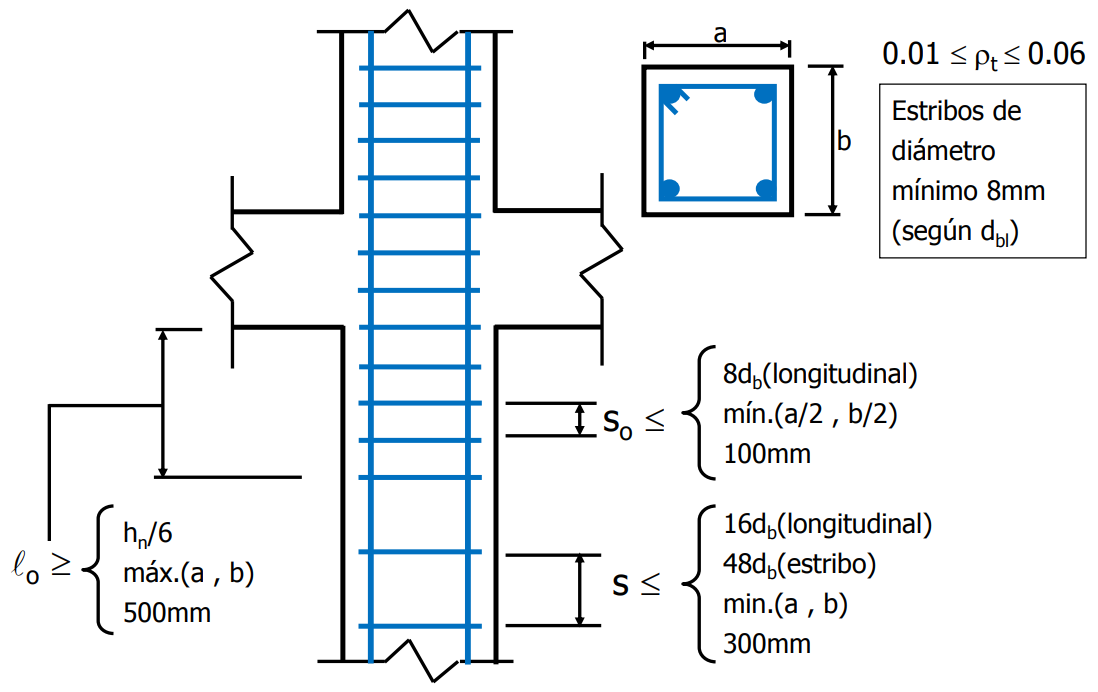
\includegraphics[width=102mm]{IMAGENES/col1.PNG}}\vspace{5mm}
    \subfigure[Sistemas de pórticos o duales]{\includegraphics[width=102mm]{IMAGENES/col2.PNG}}
   \caption*{Fuente: \cite{CAPUCP}} 
    \label{reqv}
\end{figure}
\noindent
\textit{Refuerzo transversal mínimo en columnas de pórticos}\\
\begin{align}
A_{sh} &=0.3\; \frac{s\; b_{c}\;f_{c}^{\prime}}{f_{yh}}\left[\left(\frac{A_{g}}{A_{ch}}\right)-1\right]\label{ascolmin} \\
A_{sh} &=0.09\; \frac{s\; b_{c}\; f_{c}^{\prime}}{f_{yh}}\label{ascolmin2}
\end{align}
\noindent Donde:\\
$A_{sh}$: Área de refuerzo transversal (ver figura \ref{atrans})\\
$b_{c}$: es la dimensión del núcleo confinado del elemento normal al refuerzo medida centro a centro del refuerzo de confinamiento\\
$A_{ch}$: es el área del núcleo confinado medida al exterior del refuerzo de confinamiento\\
$A_{g}$: es el área de la sección bruta de la columna\\
$s$: separación del refuerzo transversal\\
$f_{yh}$: Esfuerzo de fluencia del refuerzo transversal
\begin{figure}[h!]
    \centering
    \caption{Área de acero transversal en columnas}
    \includegraphics[scale=0.67]{IMAGENES/cc3.PNG}
    \caption*{\small Fuente: \it \cite{E-060}}
    \label{atrans}
\end{figure}
\newpage
\begin{theo}[Art. 21.6.4.1 (c) E-060 :]{thm:ca1}
Cuando la resistencia de diseño del núcleo de la sección transversal del elemento satisface los requisitos de las combinaciones de carga de diseño, incluyendo el efecto sísmico, no es necesario satisfacer la ecuación \ref{ascolmin}.
\end{theo}

\noindent En el presente caso de estudio la altura libre de mayor longitud se encuentra en el primer piso $h_{n}=3.3\;m-0.4\;m=\fpeval{3.3-0.4}\;m$
:\\
La longitud de confinamiento sera el mayor de:
\begin{itemize}
\item $h_{n} / 6= 2.9\;m/6 = 48.3\mathrm{~cm}$
\item $\max (b_{c},h_{c})= 65\mathrm{~cm}$
\item $50 \mathrm{~cm}$
\end{itemize}
La condición (b) es la mas critica por lo tanto se confinara 65cm por encima y por debajo de la luz libre de la columna.\\
La separación en esta longitud sera el menor de:
 \begin{itemize} 
\item $6d_{b}=9.53 \mathrm{~cm}$
\item $\min (b,h)/ 3=10 \mathrm{~cm}$
\item $10 \mathrm{~cm}$
    \end{itemize} 
Se adopta 10cm.\\
La separación fuera de la longitud de confinamiento sera el menor de:
 \begin{itemize} 
\item $10d_{b}=15.88 \mathrm{~cm}$
\item $25 \mathrm{~cm}$
    \end{itemize}
Se adopta 15cm.\\
La resistencia de diseño del núcleo sera:
\FPeval{\ach}{round((\bc-2*\rec)*(\hc-2*\rec),2)}
\FPeval{\pnn}{round(0.8*0.7*(0.85*\fc*(\ach-\Ast)+\Ast*\fy)/1000,2)}
\begin{align*}
    A_{ch}&=\left ( b-2\cdot r_{e} \right )\left ( h-2\cdot r_{e} \right )= \left ( \bc-2\cdot \rec \right )\left ( \hc-2\cdot \rec \right )=\ach \mathrm{~cm^2}\\
    \phi P_{n}&=0,80 \cdot 0,70 \cdot\left[0,85 \cdot \fc \cdot\left(\ach-\Ast\right)+\fy \cdot \Ast\right]=\pnn \mathrm{~ton}
\end{align*}
La capacidad de la columna cuando se pierde el recubrimiento es suficiente para soportar las cargas amplificadas que incluyen sismo, por lo que no es necesario satisfacer la ecuación \ref{ascolmin}.\\
El área de acero transversal requerido por la ecuación \ref{ascolmin2} sera:\\
Dirección del eje fuerte:
\FPeval{\bcc}{round((\bc-2*\rec-\dest),2)}
\FPeval{\hcc}{round((\hc-2*\rec-\dest),2)}
\FPset\sep{10}
\FPeval{\asnif}{round((0.09*\sep*\bcc*\fc/\fy),2)}
\FPeval{\asniff}{round((0.09*\sep*\hcc*\fc/\fy),2)}
\begin{align*}
b_{c}&=b-2\cdot r_{e}-d_{e}=\bc-2\cdot\rec-\dest=\bcc \mathrm{~cm}\\
A_{sh} &=0.09\; \frac{\sep\cdot \bcc\cdot \fc}{\fy}=\asnif\mathrm{~cm^2}
\end{align*}
Dirección del eje débil:
\begin{align*}
b_{c}&=h-2\cdot r_{e}-d_{e}=\hc-2\cdot\rec-\dest=\hcc \mathrm{~cm}\\
A_{sh} &=0.09\; \frac{\sep\cdot \hcc\cdot \fc}{\fy}=\asniff \mathrm{~cm^2}
\end{align*}
\noindent
Por lo tanto se colocaran 4 ramas en la dirección débil por el requisito de la ecuación \ref{ascolmin2}, en la dirección fuerte se colocara 3 ramas por requisito de fuerza cortante. 
\subsubsection{Requisitos adicionales para columnas de sistemas de pórticos o duales}
Según el articulo 21.6.1 estos elementos deben cumplir con:
\FPeval{\limp}{round(0.1*\fc*\Ag/1000,2)}
\begin{enumerate}
\item[] (a): La carga axial amplificada excede $0.1\;f_{c}^{'}\;A_{g}=0.1\cdot\fc\cdot\Ag=\limp\mathrm{~ton}$
\item[] (b): La menor dimensión deber ser mínimamente $B=25 \mathrm{~cm}$
\item[] (c): La relación entre la menor dimensión y la mayor sera menor que $B/L\geq 0.25$
\end{enumerate}
\begin{figure}[hb!]
    \centering
    \caption{Columna de un sistema aporticado o dual}
    \includegraphics[trim={0 5.5cm 0 0},clip,scale=0.6]{IMAGENES/cc1.PNG}
    %\caption*{\small Fuente: \it \cite{cordova2015}}
    \label{vig}
\end{figure}
\newpage
\noindent
Según la carga axial obtenida, las columnas de los niveles 1 y 2 entrarían en esta categoría.\\
\textit{Resistencia mínima a flexión de las columnas}\\
El articulo 21.6.6.2 requiere que las resistencias a flexión de las columnas en las caras de los nudos deben satisfacer la ecuación (21-1) de la \cite{E-060}:
\begin{align}
\sum M_{nc}\geq 1.2\sum M_{nv}
\end{align}
\noindent Donde:\\
$M_{nc}$: suma de los momentos nominales de flexión de las columnas que llegan al nudo, evaluados en las caras del nudo.   La resistencia a la flexión de la columna debe calcularse para  la  fuerza  axial  amplificada,  consistente  con la  dirección  de  las  fuerzas  laterales consideradas, que conduzca a la resistencia a la flexión más baja.\\
$M_{nv}$: suma de los momentos resistentes nominales a flexión de las vigas que llegan al nudo, evaluados en las caras del nudo.\\
\begin{figure}[h!]
    \centering
    \caption{Criterio columna fuerte-viga débil}
    \includegraphics[scale=0.5]{IMAGENES/cc2.PNG}
    %\caption*{\small Fuente: \it \cite{cordova2015}}
    \label{vig}
\end{figure}
\FPset\bsec{25}
\FPset\hsec{40}
\FPeval\asec{round(2*1.98,2)}
\FPeval\dsec{round(\hsec-6,2)}
\FPeval{\mnsec}{round((\asec*\fy*(\dsec-\asec*\fy/(1.7*\fc*\bsec)))/100000,2)}
\FPeval\mnsecd{round(1.2*2*\mnsec,2)}
\noindent La resistencia a la flexión de las vigas secundarias (25x40) que llegan a la columna considerando 2$\phi$5/8" como armado sera:
$$
M_{n}=A_{s}\cdot f_{y}\left ( d-\frac{A_{s}\cdot f_{y}}{1.7\cdot f_{c}^{'}\cdot b} \right )$$
$$
M_{n}=\asec \cdot \fy\left ( \dsec-\frac{\asec\cdot \fy}{1.7\cdot\fc \cdot \bsec} \right )=\mnsec\;\mathrm{~ton.m} 
$$
\FPset\mncol{13.05}
\FPeval\mncoll{round(2*\mncol,2)}
\noindent 
Del diseño por capacidad la menor resistencia de la columna en los pisos 1 y 2 resulta 13.05 ton.m.
\begin{align*}
\sum M_{nc}&\geq 1.2\sum M_{nv}\\
\left ( \mncol+\asnifmncol \right )&\geq 1.2\left ( \mnsec+\mnsec \right )\\
\mncoll \mathrm{~ton.m} &\geq \mnsecd \mathrm{~ton.m}
\end{align*}
\noindent Se cumple el criterio de columna fuerte viga débil.\\
\textit{Refuerzo transversal en nudos}
\begin{theo}[Art. 21.7.3 E-060 :]{thm:ca1}
Dentro  del  nudo  deben  colocarse  estribos  cerrados  de  confinamiento  como refuerzo transversal, tal como lo específica 21.6.4, a menos que dicho nudo esté confinado por elementos estructurales, como lo específica 21.7.3.2.\\
Cuando existan elementos que llegan en los cuatro lados del nudo y el ancho de cada elemento mide por lo menos tres cuartas partes del ancho de la columna, debe disponerse refuerzo transversal igual, por lo menos a la mitad de la cantidad requerida en 21.6.4.1, dentro del peralte del elemento de menor altura. En estos lugares, se permite que el espaciamiento especificado en 21.6.4.2 se  incremente a 150 mm.
\end{theo}
\noindent
\textit{Resistencia a cortante en nudos}\\
Art. 21.7.4: La  resistencia  Vn en  el  nudo  no  debe  ser  mayor  que  las  fuerzas  especificadas  a continuación, para concreto de peso normal:
\begin{flalign}
&\textup{Para nudos confinados en las cuatro caras:}\quad \text{\makebox[7cm]{\dotfill $5.3\sqrt{f_{c}^{\prime}}\;A_{j}$}}&&\\
&\textup{Para nudos confinados en tres caras o en dos caras opuestas:}
\quad \text{\makebox[3.7cm]{\dotfill $4.0\sqrt{f_{c}^{\prime}}\;A_{j}$}}&&\\
&\textup{Para otros casos:} \quad \text{\makebox[11.6cm]{\dotfill $3.2\sqrt{f_{c}^{\prime}}\;A_{j}$}}&&
\end{flalign}
\newpage
Se considera que un elemento (viga) proporciona confinamiento al nudo si al menos las tres cuartas partes de la cara lateral del nudo está cubierta por el elemento que llega al nudo.
\begin{figure}[h!]
    \centering
    \subfigure[Tipos de nudos]{\includegraphics[width=150mm]{IMAGENES/cc6.PNG}}\vspace{10mm}
    \subfigure[Área efectiva del nudo]{\includegraphics[width=100mm]{IMAGENES/cc4.PNG}}
    \caption{Resistencia a cortante de nudos}
    \label{reqv}
\end{figure}
\newpage
\begin{figure}[ht!]
    \centering
    \subfigure[Equilibrio de fuerzas en el nudo]{\includegraphics[width=80mm]{IMAGENES/cc5.PNG}}\hspace{10mm}
    \subfigure[Cortante en columna]{\includegraphics[width=60mm]{IMAGENES/cc7.PNG}}
    \caption{Resistencia a cortante de nudos}
    \label{reqn}
\end{figure}
\textit{Refuerzo transversal en nudos}
\begin{theo}[Area efectiva del nudo Art. 21.7.4.1 E-060 :]{thm:ca1}
$A_{j}$ es el área efectiva de la sección transversal dentro del nudo en la dirección de análisis, calculada  como  el  producto  de  la  profundidad  del  nudo  por su  ancho  efectivo. La profundidad del nudo es la dimensión total de la columna en la dirección de análisis. El ancho efectivo del nudo es el ancho total de la columna, excepto que cuando la viga llega a una columna más ancha que ésta, el ancho efectivo del nudo no debe exceder el menor de (a) y (b):
\begin{enumerate}
\item[] (a): el ancho de la viga más la profundidad del nudo.  Si el ancho difiere a ambos lados de la columna, se utilizará el promedio de ellos.
\item[] (b): dos veces la distancia del eje longitudinal de la viga al borde más cercano de la columna
\end{enumerate}
\end{theo}
\noindent 
En este caso se trata de un columna exterior, por tanto la profundidad del nudo es igual al ancho de la columna \bc cm y teniendo en cuenta que el ancho de la viga es de \bsec cm el ancho efectivo sera el menor de:
\FPeval{\aa}{round(\bsec+\bc,0)}
\FPeval{\xx}{round(0.5*\bsec,2)}
\FPeval{\bb}{round(\bsec+\xx*2,0)}
\begin{enumerate}
\item[] (a): \bsec+\bc=\aa cm
\item[] (b): \bsec+$2x$=\bsec+\xx=\bb cm
\end{enumerate}
\FPmin\cc{\aa}{\bb}
El área efectiva y la resistencia a cortante del nudo respectivamente sera:
\FPeval{\aj}{round(\cc*\bc,2)}
\FPeval{\vnu}{round(0.5*4*\rc*\aj/1000,2)}
\begin{align*}
A_{j}&=\cc\cdot\bc=\aj \mathrm{~cm^2}\\
\phi V_{n}&=0.85\cdot4.0\cdot\sqrt{\fc}\cdot\aj=\vnu \mathrm{~ton}
\end{align*}
\noindent La cortante en la columna producto de la fluencia de las vigas sera:
\FPset\hcol{2.4}
\FPeval\vcoln{round(1.25*2*\mnsec/\hcol,2)}
\begin{align}
V_{col}&=2\;\frac{M_{pi}+M_{pd}}{H}\\
V_{col}&=2\cdot\frac{1.25\cdot2\cdot\mnsec}{\hcol}=\vcoln\notag \mathrm{~ton}
\end{align}
\noindent
Donde:\\
$M_{pi},M_{pd}$: Momentos de vigas a cada lado del nudo para 1.25$f_{y}$ (Art. 21.7.2.1)\\
$H$: Altura entre puntos de inflexión de la columna (ver figura \ref{reqn})\\
\noindent La cortante producida en el nudo según 21.7.4.3 sera:
\FPeval{\vnuu}{round(1.25*2*\asec*\fy/1000-\vcoln,2)}
\begin{align}
V_{u}&=1.25\left ( A_{s1}+A_{s2} \right )f_{y}-V_{col}\\
V_{u}&=1.25\left ( \asec+\asec \right )\cdot \fy-\vcoln \mathrm{~ton}=\vnuu\mathrm{~ton}\notag
\end{align}
\noindent Se cumple con $\phi V_{n}\geq V_{u}$.

\newpage
\subsection{Diseño de muros de corte o placas}
\subsubsection{Diseño a flexocompresión}
La cuantía mínima según el artículo 11.10.10.3: $\rho_{\mathrm{v}}=0.0025$\\
Para el muro en estudio de espesor 25cm se colocara en el alma doble malla de 3/8"@20cm lo que representa una cuantía de:
\FPset\svwall{20}
\FPset\ewall{25}
\FPset\asvwall{0.71}
\FPset\nfvwall{2}
\FPeval\pvwall{round(2*\asvwall/(\ewall*\svwall),4)}
\begin{align*}
\rho_{v} =\frac{n\cdot A_{sh}}{e\cdot s}=\frac{\nfvwall\cdot \asvwall}{\ewall\cdot \svwall}=\pvwall
\end{align*}
\noindent
Donde:\\
$e$: Espesor del muro\\
$\rho_{v}$: Cuantía vertical en el muro\\
$A_{sh}$: Área de la varilla utilizada\\
$n$: numero de capas\\
$s$: separación del refuerzo.\\
En el borde izquierdo de espesor constante se coloco 6 $\phi$ 5/8" en una longitud de 30cm, en el borde derecho que también funciona como una columna de 25x65cm se coloco una cuantía de 1\% haciendo un total de 10 $\phi$ 5/8", con el armado propuesto se hace la verificación en flexocompresión: 
\begin{figure}[h!]
    \centering
    \caption{Diagrama de interacción del muro PL-1}
    \includegraphics[scale=0.67]{IMAGENES/pl2.pdf}
    %\caption*{\small Fuente: \it \cite{E-060}}
    \label{atrans}
\end{figure}

\FPset\agwall{6750}
\FPeval{\limwall}{round(0.1*\fc*\agwall/1000,2)}
\noindent El limite de carga axial es:
\begin{align*}
0.1\;f_{c}^{'}\;A_{g}=0.1\cdot\fc\cdot\agwall=\limwall\mathrm{~ton}
\end{align*}
Las cargas ultimas amplificadas están por debajo de este valor por lo que no seria necesario las verificaciones que se mencionan a continuación para muros en flexocompresión.
\subsubsection{Diseño de elementos especiales de borde}
Los elementos de borde en la zona en compresión deben ser confinados cuando la profundidad del eje neutro exceda:
\begin{align}
c \geq \frac{l_{m}}{600\left(\delta_{u} / h_{m}\right)}  
\end{align}
\noindent
Según el artículo 21.9.7.4 este criterio solo aplica para muros continuos y diseñados para tener una sola sección critica para flexión y carga axial.\\
Si se requiere elementos de borde especiales la separación máxima $s_{0}$ dentro del núcleo confinado según 21.9.7.6 (e) será el menor de:
\begin{enumerate}
\item[] (a): $10 d_{b}$
\item[] (b): $\min \left(e, l_{c}\right)$
\item[] (c): $25 \mathrm{~cm}$
\end{enumerate}
\noindent
La longitud del elemento de borde debe cumplir con 21.9.7.6 (a) y no será menor que:
\begin{enumerate}
\item[] (a): $c/2$
\item[] (b): $c-0,1 \cdot l_{m}$
\end{enumerate}
La altura de confinamiento debe cumplir con 21.9.7.4 y no será menor del mayor valor obtenido con:
\begin{enumerate}
\item[] (a): $l_{m}$
\item[] (b): $ \displaystyle\frac{M_{u}}{4 \cdot V_{u}}$
\end{enumerate}
\noindent
Donde no se requiera elementos de borde confinados se debe cumplir con 21.9.7.7:\\
\noindent
La separación máxima del refuerzo transversal no deberá exceder 16 veces el diámetro de la barra longitudinal, 48 veces el diámetro del estribo y la menor dimensión del elemento en compresión.
\begin{enumerate}
\item[] (a): $16 d_{b}$
\item[] (b): $48 d_{e}$
\item[] (c): $\min (b, h)$
\item[] (d): $25 \mathrm{~cm}$
\end{enumerate}

\begin{figure}[h!]
    \centering
    \caption{Elemento especial de borde}
    \includegraphics[scale=0.67]{IMAGENES/pl1.PNG}
    %\caption*{\small Fuente: \it \cite{E-060}}
    \label{atrans}
\end{figure}

En cualquier caso, los estribos deberán cumplir con:
\begin{itemize}
  \item Ninguna barra longitudinal esté separada a más de $150 \mathrm{~mm}$ libres de una barra apoyada lateralmente. (figura 13)

  \item El refuerzo transversal debe disponerse mediante estribos cerrados de confinamiento sencillos o múltiples. Se pueden usar grapas suplementarias del mismo diámetro de barra y con el mismo espaciamiento que los estribos cerrados de confinamiento.

  \item La distancia, centro a centro, transversal al eje del elemento, entre las ramas de estribos cerrados de confinamiento múltiples o entre las grapas suplementarias, hx, no deben exceder 350 mm medidos centro a centro.

\end{itemize}

\begin{figure}[h!]
    \centering
    \subfigure[]{\includegraphics[width=100mm]{IMAGENES/est2.PNG}}\hspace{0mm}
    \subfigure[]{\includegraphics[width=50mm]{IMAGENES/est1.PNG}}
    \caption{Requisitos en estribos}
    \label{reqv}
\end{figure}

\subsubsection{Diseño a cortante}

\noindent Peralte efectivo del muro (Art. 21.9.4.5)
\begin{align}
    d=0,80 \cdot l_{w}
\end{align}
Contribución del concreto a cortante (Art. 11.10.5)
\begin{align}
   V_{c}=A_{c w} \cdot\left(\alpha_{c} \cdot \sqrt{f_{c}^{\prime}}\right)
\end{align}
\noindent
Donde:\\
$A_{c w}:$ Área resistente a cortante (área del alma) $A_{c w}=d \cdot e$\\
$e:$ Espesor del muro Donde $\alpha_{c}$ depende de la esbeltez del muro según:
\begin{align*}
&\alpha_{c} \text { es } 0,80 \text { para } \frac{h_{m}}{l_{w}} \leq 1,5 ; \\
&\alpha_{c} \text { es } 0,53 \text { para } \frac{h_{m}}{l_{w}}>2 \\
&\alpha_{c} \text { varia linealmente entre } 0,80 \text { y } 0,53 \text { para } \frac{h_{m}}{l_{w}} \text { entre } 1,5 \text { y } 2,0.
\end{align*}

\begin{figure}[h!]
    \centering
    \subfigure[]{\includegraphics[width=65mm]{IMAGENES/wall2.PNG}}\hspace{10mm}
    \subfigure[]{\includegraphics[width=75mm]{IMAGENES/walls.PNG}}
    \caption{Diseño a cortante de muros}
    \label{corw}
\end{figure}

Cortante máxima según el Art. 11.10.4
\begin{align}
    V_{n} \leq 2,6 \cdot \sqrt{f_{c}^{\prime}} \cdot A_{c w}
\end{align}
Cortante máxima en los estribos según la Ecu. 11-2
\begin{align}
    V_{s, \max }=V_{n}-V_{c}
\end{align}
Cortante requerida en estribos según la Ecu. 11-1
\begin{align}
    V_{s, r e q}=\frac{V_{u}-\phi_{c} \cdot V_{c}}{\phi_{c}}
\end{align}
Resistencia a corte del refuerzo horizontal según la Ecu. 11-31
\begin{align}
    V_{s}=A_{c w} \cdot \rho_{h} \cdot f_{y}
\end{align}
Cuantía de refuerzo horizontal en muro
\begin{align}
    \rho_{h}=\frac{A_{v}}{s \cdot e}
\end{align}
\noindent
Donde:\\
$A_{v}:$ Área de la varilla de refuerzo transversal\\
s : Separación del acero transversal\\
\noindent
La cortante de diseño según el Art. 21.9.5.3 se ajustará a la capacidad a flexión instalada del muro según:
\begin{align}
    V_{u}=V_{u a}\left(\frac{M_{n}}{M_{u a}}\right)
\end{align}
\noindent
Donde:\\
$V_{u a}:$ Cortante obtenido del análisis\\
$M_{u a}:$ Momento obtenido del análisis.\\
$M_{n}:$ Momento nominal obtenido para la carga axial de diseño.\\
\noindent
Esta disposición se limita al mayor valor obtenido de:
\begin{enumerate}
\item[] (a): $l_{w}$
\item[] (b): $\displaystyle\frac{M_{u}}{4 \cdot V_{u}}$
\item[] (c): Altura de los 2 primeros pisos.
\end{enumerate}
\noindent
Para el presente muro se tiene:
\FPset\lw{2.3}
\FPset\hw{16.6}
\FPeval{\esbw}{round(\hw/\lw,2)}
\FPeval{\dwall}{round(0.8*\lw,2)}
\FPeval{\acwall}{round(\ewall*\dwall*100,2)}
\begin{itemize}
    \item Longitud del muro: $l_{w}=\lw\mathrm{~m}$
    \item Altura total del muro: $h_{m}=\hw\mathrm{~m}$
    \item Esbeltez del muro: $h_{m}/l_{w}=\esbw\mathrm{~m}$
    \item Coeficiente: $\alpha_{c}=0.53 $
    \item Peralte efectivo: $d=0.8\cdot l_{w}=0.8\cdot\lw=\dwall \mathrm{~m}$
    \item Área resistente a cortante: $A_{c w}=d \cdot e=\dwall \cdot\ewall= \acwall\mathrm{~cm^2}$
\end{itemize}

Cortante resistente por el concreto según:
\FPeval{\vconw}{round(0.53*\rc*\acwall/1000,2)}
\begin{center}
$V_{c}=A_{c w} \cdot\left(\alpha_{c} \cdot \sqrt{f_{c}^{\prime}}\right)=\acwall \cdot 0.53 \cdot \sqrt{\fc}=\vconw\mathrm{~ton}$
\end{center}

\FPset\puw{114.28}
\FPset\muw{62.72}
\FPset\vuw{18}
\FPset\mnwall{336.32}
Solicitaciones para la combinación critica 1.25(CM+CV)+SX:
\begin{itemize}
    \item Carga axial: $P_{u}=\puw\mathrm{~ton}$
    \item Momento: $M_{ua}=\muw\mathrm{~ton.m}$
    \item Cortante: $V_{ua}=\vuw\mathrm{~ton}$
\end{itemize}
El momento nominal del muro para la carga axial obtenida según la figura \ref{corw} (a) resulta $M_{n}=\mnwall\mathrm{~ton.m}$, el factor de amplificación por capacidad del muro sera:
\FPeval{\ampw}{round(\mnwall/\muw,2)}
\begin{center}
$\displaystyle\frac{M_{n}}{M_{u a}}=\frac{\mnwall}{\muw}=\ampw$
\end{center}
Este valor según \cite{E-060} debe ser menor que el factor de reducción R, sin embargo este valor se puede limitar a 2.5 que es el factor de sobreresistencia en edificios de muros según normas extranjeras, el \cite{ACI19} limita este valor a 3 pero incluye el factor de amplificación por modos superiores.\\
\noindent Por lo tanto, la cortante ultima de diseño sera igual a:
\FPeval{\vuuw}{round(2.5*\vuw,2)}
\begin{center}
 $\displaystyle V_{u}=V_{u a}\left(\frac{M_{n}}{M_{u a}}\right)=\vuw\cdot2.5=\vuuw\mathrm{~ton}$
\end{center}
Cortante requerido por el refuerzo horizontal:
\FPeval{\vswa}{round((\vuuw-0.85*\vconw)/0.85,2)}
\begin{center}
    $\displaystyle V_{s, r e q}=\frac{V_{u}-\phi_{c} \cdot V_{c}}{\phi_{c}}=\frac{\vuuw-0.85 \cdot \vconw}{0.85}=\vswa\mathrm{~ton}$
\end{center}
Se propone una cuantía mínima igual a la colocada como acero vertical en el alma que consiste en una doble malla de 3/8"@20cm.
La resistencia al cote por el refuerzo horizontal sera:
\FPeval{\vsswa}{round((\acwall*\pvwall*\fy)/1000,2)}
\begin{center}
    $\displaystyle V_{s}=A_{c w} \cdot \rho_{h} \cdot f_{y}=\acwall \cdot \pvwall \cdot \fy=\vsswa\mathrm{~ton}$
\end{center}
La resistencia a cortante nominal del muro sera:
\FPeval{\vnwall}{round(\vconw+\vsswa,2)}
\begin{center}
    $\displaystyle V_{n}=V_{c}+V_{s}=\vconw+\vsswa=\vnwall\mathrm{~ton}$
\end{center}
La cortante nominal máxima del muro sera:
\FPeval{\vnmaxwall}{round(2.6*\rc*\acwall/1000,2)}
\begin{center}
    $\displaystyle V_{n,max} =2,6 \cdot \sqrt{f_{c}^{\prime}} \cdot A_{c w}=2,6 \cdot \sqrt{\fc} \cdot \acwall=\vnmaxwall\mathrm{~ton}$
\end{center}
La condición $V_{n}\leq V_{n,max}$ se cumple.
Finalmente la cortante resistente sera:
\FPeval{\vnuwall}{round(\vnwall*0.85,2)}
\begin{center}
    $\displaystyle \phi V_{n}=0.85\cdot\vnwall= \vnuwall\mathrm{~ton}$
\end{center}
La condición $\phi V_{n}\leq V_{u}$ se cumple.
\subsection{Diseño de muro de sótano}
Del estudio de mecánica de suelos se obtiene los siguientes parámetros geotécnicos:
\FPset\gamas{1.9}
\FPset\ko{0.431}
\FPset\kp{3.639}
\FPset\ka{0.275}
\begin{itemize}
    \item Densidad del suelo: $\gamma =\gamas\mathrm{~ton/m^3}$
    \item Coeficiente de presión en reposo: $K_{o}=\ko$
    \item Coeficiente de presión pasiva: $K_{p}=\kp$
    \item Coeficiente de presión activa: $K_{a}=\ka$
\end{itemize}
Las cotas del muro con respecto al nivel de la cara superior de cimentación de la parte mas profunda del edificio son:
\FPset\zone{3.3}
\FPset\ztwo{11.2}
\FPset\zthree{5.8}
\FPeval{\hmcon}{round(\ztwo-\zone,2)}
\begin{itemize}
    \item Cota inferior del muro: $z_{1} =\zone\mathrm{~m}$
    \item Cota superior del muro: $z_{2}=\ztwo\mathrm{~m}$
    \item Cota del segundo nivel: $z_{3}=\zthree\mathrm{~m}$
    \item Altura total del muro: $H=z_{2}-z_{1}=\hmcon\mathrm{~m}$
\end{itemize}
\FPset\wsc{2}
\FPset\wscr{0.2}
Se considero una sobrecarga de un edificio de 2 niveles en la parte posterior del muro equivalente a $w_{sc}=\wsc\mathrm{~ton/m^2}$ y una carga permanente en el primer de $w_{sc}^{\prime}=\wscr\mathrm{~ton/m^2}$.\\
Para ingresar la carga variable en ETABS es necesario definir una ecuación de la forma:
\begin{align}
    P=Ax+By+Cz+D
\end{align}
Dado que la carga solo cambia en la dirección z los coeficientes A y B resultan cero.\\
Para la presión en la parte posterior del muro se aplican las condiciones de frontera y se obtiene los coeficientes C y D:
\FPeval{\equone}{round(\ko*\wsc+\ko* \gamas * \hmcon,2)}
\FPeval{\equtwo}{round(\ko*\wsc,2)}
\FPeval{\cwall}{round((\equtwo-\equone)/(\ztwo-\zone),2)}
\FPeval{\dwall}{round(\equone-\zone*\cwall,2)}
\FPeval{\hright}{round(\zthree-\zone,2)}
\begin{align}
\shortintertext{Presión en la base del muro ($z=\zone$):} K_{o}\cdot w_{sc}+K_{o}\cdot \gamma \cdot H&=C(z_{1})+D\notag\\
\ko\cdot \wsc+\ko\cdot \gamas \cdot \hmcon&=C(\zone)+D\notag\\
\equone&=\zone\; C+D\label{eq1}\\ \shortintertext{Presión en la cota superior del muro ($z=\ztwo$):}
K_{o}\cdot w_{sc}&=C(z_{2})+D\notag\\
\ko\cdot \wsc&=C(\ztwo)+D\notag\\
\equtwo&=\ztwo\; C+D\label{eq2}
\end{align}
\noindent Combinando \ref{eq1} y \ref{eq2} se obtiene $C=\cwall\mathrm{~ton/m^3}$ y $D=\dwall\mathrm{~ton/m^2}$.\\
Se procede de manera similar para la presión que ejerce en sentido contrario el suelo de relleno debajo del segundo nivel con una altura igual a $h=z_{3}-z_{1}=\hright$.
  \begin{spacing}{2}
  \leftskip 1.27cm
  \rightskip 1.27cm
\noindent Se define el coeficiente de empuje como la relación entre la tensión efectiva horizontal y la vertical, y en el caso de que no exista deformación lateral, se denomina coeficiente de empuje al reposo, $K_{o}$. De esta forma se podría calcular el empuje sobre un muro que no se deformara lo más mínimo. Sería el caso de un muro de sótano en edificación. Pero los muros no son infinitamente rígidos, se deforman, y dependiendo de si la deformación lateral es negativa (el terreno “se descomprime”) o positiva (el terreno “se comprime”), tendríamos los denominados empujes activos $K_{a}$, o pasivos $K_{p}$, $\left ( k_{a}< k_{o} < k_{p}\right )$. Para movilizar el empuje pasivo son necesarios movimientos del muro contra el terreno muy superiores a los necesarios para llegar a una situación de empuje activo. Cuando el empuje pasivo es favorable, debido a la imprecisión en la determinación de su valor real, por seguridad suele despreciarse su efecto o bien se aplica un coeficiente reductor (por ejemplo, de 1,5). \cite{empuje}
  \end{spacing}

\begin{figure}[h!]
    \centering
    \caption{coeficientes de empujes}
    \includegraphics[scale=0.55]{IMAGENES/empuje.jpg}
    \caption*{\small Fuente: \it \cite{empuje}}
    \label{atrans}
\end{figure} 
  
\FPset\kpp{1.8}

\noindent Por lo mencionado en el anterior párrafo se hará el calculo de la presión que disminuye las solicitaciones en la pantalla del muro con un coeficiente de empuje pasivo reducido de $K_{p}^{\prime}=\kpp$
\FPeval{\equoner}{round(\kpp*\wscr+\kpp* \gamas * \hright,2)}
\FPeval{\equtwor}{round(\kpp*\wscr,2)}
\FPeval{\cwallr}{round((\equtwor-\equoner)/(\zthree-\zone),2)}
\FPeval{\dwallr}{round(\equoner-\zone*\cwallr,2)}
\begin{align}
\shortintertext{Presión en la base del muro ($z=\zone$):} K_{p}^{\prime}\cdot w_{sc}^{\prime}+K_{p}^{\prime}\cdot \gamma \cdot h&=C(z_{3})+D\notag\\
\kpp\cdot \wscr+\kpp\cdot \gamas \cdot \hright&=C(\zone)+D\notag\\
\equoner&=\zone\; C+D\label{eq3}\\ \shortintertext{Presión en el segundo nivel ($z=\zthree$):}
K_{p}^{\prime}\cdot w_{sc}^{\prime}&=C(z_{3})+D\notag\\
\kpp\cdot \wscr&=C(\zthree)+D\\
\equtwor&=\zthree\; C+D\label{eq4}
\end{align}
\noindent
Combinando \ref{eq3} y \ref{eq4} se obtiene $C=\cwallr\mathrm{~ton/m^3}$ y $D=\dwallr\mathrm{~ton/m^2}$.\\
La norma \cite{E-060} en el articulo 9.2.5 menciona que las combinaciones para el diseño de elementos sujetos a empujes de tierra sera:
\begin{align*}
    U&=1.4CM+1.7CV\\
    U&=1.4CM+1.7CV+1.7CE\\
    U&=0.9CM+1.7CE
\end{align*}
\noindent Donde:\\
CE: empuje lateral de los suelos.
\begin{figure}[h!]
    \centering
    \caption{Envolvente de momentos en la dirección horizontal de la pantalla}
    \includegraphics[scale=0.6]{IMAGENES/m11.PNG}
    %\caption*{\small Fuente: \it \cite{empuje}}
    \label{m11}
\end{figure} 

\begin{figure}[h!]
    \centering
    \caption{Envolvente de momentos en la dirección vertical de la pantalla}
    \includegraphics[scale=0.6]{IMAGENES/m22.PNG}
    %\caption*{\small Fuente: \it \cite{empuje}}
    \label{m22}
\end{figure} 
\newpage
\begin{figure}[h!]
    \centering
    \caption{Envolvente de corte de la pantalla}
    \includegraphics[scale=0.6]{IMAGENES/v23.PNG}
    %\caption*{\small Fuente: \it \cite{empuje}}
    \label{v23}
\end{figure}
\newpage
\noindent
La norma \cite{E-060} menciona en el articulo 10.5.4 que para losas estructurales donde el refuerzo se distribuye en 2 capas la cuantía mínima en la cara en tracción debe ser mayor a 0.0012.\\
Como acero horizontal se colocara doble malla de 1/2"@25cm lo que representa una cuantía de:
\FPset\shwallc{25}
\FPset\ewallc{30}
\FPset\ashwallc{1.27}
\FPset\nfhwallc{2}
\FPeval\pvwallc{round(\ashwallc/(\ewallc*\shwallc),4)}
\FPset\bwa{100}
\FPeval\ashtw{round(\ashwallc*\bwa/\shwallc,2)}
\FPeval\dwa{round(\ewallc-9,2)}
\FPeval{\mnhw}{round((0.9*\ashtw*\fy*(\dwa-\ashtw*\fy/(1.7*\fc*\bwa)))/100000,2)}
\begin{align*}
\rho_{v} =\frac{A_{sh}}{e\cdot s}=\frac{\ashwallc}{\ewallc\cdot \shwallc}=\pvwallc
\end{align*}
\noindent Para el calculo de la resistencia a la flexión de la pantalla en la dirección horizontal se considero 1m de ancho de losa y un peralte efectivo de $d=e-9\mathrm{~cm}$ dado que la norma \cite{E-060} menciona en el articulo 7.7 que el recubrimiento mínimo para concreto colocado en contacto con el suelo es mínimo 7cm.
$$
M_{nh}=\phi\cdot A_{s}\cdot f_{y}\left ( d-\frac{A_{s}\cdot f_{y}}{1.7\cdot f_{c}^{'}\cdot b} \right )$$
$$
A_{s}=\frac{A_{sh}\cdot b}{s}=\frac{\ashwallc\cdot\bwa}{\shwallc}=\ashtw\mathrm{~cm^2}$$
$$
M_{n}=0.9\cdot \ashtw \cdot \fy\left ( \dwa-\frac{\ashtw\cdot \fy}{1.7\cdot\fc \cdot \bwa} \right )=\mnhw\;\mathrm{~ton.m} 
$$
En la figura \ref{m11} se muestra que el máximo momento es de $3.72\mathrm{~ton.m}$ por lo que se cumple con $\phi M_{n}\leq M_{u}$.

Como acero vertical corrido se coloca doble malla de 5/8"@20cm:
\FPset\asvwallc{1.98}
\FPset\nfvwallc{2}
\FPset\svwallc{20}
\FPeval\asvtw{round(\asvwallc*\bwa/\svwallc,2)}
\FPeval{\mnvw}{round((0.9*\asvtw*\fy*(\dwa-\asvtw*\fy/(1.7*\fc*\bwa)))/100000,2)}
$$
A_{sv}=\frac{A_{sh}\cdot b}{s}=\frac{\nfvwallc\cdot\asvwallc\cdot\bwa}{\svwallc}=\asvtw\mathrm{~cm^2}$$
$$
M_{n}=0.9\cdot \asvtw \cdot \fy\left ( \dwa-\frac{\asvtw\cdot \fy}{1.7\cdot\fc \cdot \bwa} \right )=\mnvw\;\mathrm{~ton.m} 
$$
En la base del muro se coloca refuerzo adicional en forma de bastones con varillas de 3/4"@20cm, con lo que el momento resistente sera:
\FPset\astwallc{2.85}
\FPset\svtwallc{20}
\FPeval\asvttw{round(\asvwallc*\bwa/\svwallc+\astwallc*\bwa/\svtwallc,2)}
\FPeval{\mnvtw}{round((0.9*\asvttw*\fy*(\dwa-\asvttw*\fy/(1.7*\fc*\bwa)))/100000,2)}
$$
A_{sv}=\frac{A_{sh1}\cdot b}{s_{1}}+\frac{A_{sh2}\cdot b}{s_{2}}=\frac{\asvwallc\cdot\bwa}{\svwallc}+\frac{\astwallc\cdot\bwa}{\svtwallc}=\asvttw\mathrm{~cm^2}$$
$$
M_{n}=0.9\cdot \asvttw \cdot \fy\left ( \dwa-\frac{\asvttw\cdot \fy}{1.7\cdot\fc \cdot \bwa} \right )=\mnvtw\;\mathrm{~ton.m} 
$$
Según los resultados de la figura \ref{m22} la condición: $\phi M_{n}\leq M_{u}$ no se cumple estrictamente, pero se acepta el diseño dado las incertidumbres que conlleva el calculo de las presiones en el suelo y que se adopto valores conservadores en el calculo.\\
Así mismo se observa que el punto de corte teórico del bastón es aproximadamente 0.85m, a la cual debe sumarse el mayor valor de $12d_{b}$ y $d$ para obtener la longitud final del bastón debiéndose cumplir también sea mayor a la longitud de desarrollo $l_{d}$, con lo anteriormente mencionado se adopta un bastón de 1.10m medido desde la cara superior de la cimentación.\\
La resistencia a cortante del muro sera:
\FPeval{\vconwc}{round(0.85*0.53*\rc*\bwa*\dwa/1000,2)}
\begin{center}
$V_{c}=\phi_{c}\cdot0.53\cdot\sqrt{f_{c}^{\prime}}\cdot b\cdot d=0.85\cdot0.53\cdot\sqrt{\fc}\cdot\bwa\cdot\dwa=\vconwc\mathrm{~ton}$
\end{center}
Según los resultados de la figura \ref{v23} fuera de la zona de concentración de esfuerzos donde existe una columna la condición $\phi V_{n}\leq V_{u}$ se cumple, donde $V_{u}$ se lee a una distancia ``d'' de la cara.
\begin{figure}[h!]
    \caption{Esquema de armado en muro de contención}
    \centering
    

\tikzset{every picture/.style={line width=0.75pt}} %set default line width to 0.75pt        

\begin{tikzpicture}[x=0.75pt,y=0.75pt,yscale=-1.7,xscale=1.7]
%uncomment if require: \path (0,294); %set diagram left start at 0, and has height of 294

%Straight Lines [id:da02765995054139414] 
\draw [color={rgb, 255:red, 251; green, 65; blue, 65 }  ,draw opacity=1 ]   (200,50) -- (200,210) ;
%Straight Lines [id:da7174171508595149] 
\draw [color={rgb, 255:red, 251; green, 65; blue, 65 }  ,draw opacity=1 ]   (220,50) -- (220,129.11) -- (220,210) ;
%Straight Lines [id:da16123548373676821] 
\draw [color={rgb, 255:red, 250; green, 185; blue, 86 }  ,draw opacity=1 ]   (190,170) -- (350,170) ;
%Straight Lines [id:da6876756264722994] 
\draw [color={rgb, 255:red, 250; green, 185; blue, 86 }  ,draw opacity=1 ]   (190,110) -- (195.44,110) -- (350,110) ;
%Straight Lines [id:da5345592683211662] 
\draw [color={rgb, 255:red, 250; green, 185; blue, 86 }  ,draw opacity=1 ]   (190,70) -- (350,70) ;
%Straight Lines [id:da4775969576589747] 
\draw [color={rgb, 255:red, 74; green, 144; blue, 226 }  ,draw opacity=1 ]   (210,100) -- (210,210) ;
%Straight Lines [id:da9167199448755778] 
\draw [color={rgb, 255:red, 250; green, 185; blue, 86 }  ,draw opacity=1 ]   (190,90) -- (350,90) ;
%Straight Lines [id:da3839448632427229] 
\draw [color={rgb, 255:red, 250; green, 185; blue, 86 }  ,draw opacity=1 ]   (190,130) -- (350,130) ;
%Straight Lines [id:da5995694819521058] 
\draw [color={rgb, 255:red, 250; green, 185; blue, 86 }  ,draw opacity=1 ]   (190,150) -- (350,150) ;
%Straight Lines [id:da5283245755076051] 
\draw [color={rgb, 255:red, 250; green, 185; blue, 86 }  ,draw opacity=1 ]   (190,190) -- (350,190) ;
%Straight Lines [id:da7631301711528842] 
\draw [color={rgb, 255:red, 251; green, 65; blue, 65 }  ,draw opacity=1 ]   (240,50) -- (240,210) ;
%Straight Lines [id:da4503876477958497] 
\draw [color={rgb, 255:red, 251; green, 65; blue, 65 }  ,draw opacity=1 ]   (260,50) -- (260,129.11) -- (260,210) ;
%Straight Lines [id:da2523584293852721] 
\draw [color={rgb, 255:red, 74; green, 144; blue, 226 }  ,draw opacity=1 ]   (250,100) -- (250,210) ;
%Straight Lines [id:da26629173415335905] 
\draw [color={rgb, 255:red, 251; green, 65; blue, 65 }  ,draw opacity=1 ]   (280,50) -- (280,210) ;
%Straight Lines [id:da47826869434014285] 
\draw [color={rgb, 255:red, 251; green, 65; blue, 65 }  ,draw opacity=1 ]   (300,50) -- (300,129.11) -- (300,210) ;
%Straight Lines [id:da6746906726566013] 
\draw [color={rgb, 255:red, 74; green, 144; blue, 226 }  ,draw opacity=1 ]   (290,100) -- (290,210) ;
%Straight Lines [id:da9467302657021419] 
\draw [color={rgb, 255:red, 251; green, 65; blue, 65 }  ,draw opacity=1 ]   (320,50) -- (320,210) ;
%Straight Lines [id:da9845424515843693] 
\draw [color={rgb, 255:red, 251; green, 65; blue, 65 }  ,draw opacity=1 ]   (340,50) -- (340,129.11) -- (340,210) ;
%Straight Lines [id:da6511672329596734] 
\draw [color={rgb, 255:red, 74; green, 144; blue, 226 }  ,draw opacity=1 ]   (330,100) -- (330,210) ;
%Straight Lines [id:da7546784093194612] 
\draw [color={rgb, 255:red, 74; green, 144; blue, 226 }  ,draw opacity=1 ]   (230,100) -- (230,210) ;
%Straight Lines [id:da9453033800840973] 
\draw [color={rgb, 255:red, 74; green, 144; blue, 226 }  ,draw opacity=1 ]   (270,100) -- (270,210) ;
%Straight Lines [id:da9828731672607554] 
\draw [color={rgb, 255:red, 74; green, 144; blue, 226 }  ,draw opacity=1 ]   (310,100) -- (310,210) ;
%Shape: Rectangle [id:dp27404908662152794] 
\draw  [color={rgb, 255:red, 139; green, 239; blue, 108 }  ,draw opacity=1 ][dash pattern={on 4.5pt off 4.5pt}] (190,50) -- (350,50) -- (350,210) -- (190,210) -- cycle ;
%Shape: Rectangle [id:dp10059166024042598] 
\draw  [color={rgb, 255:red, 139; green, 87; blue, 42 }  ,draw opacity=1 ][dash pattern={on 4.5pt off 4.5pt}] (190,210) -- (350,210) -- (350,240) -- (190,240) -- cycle ;
%Straight Lines [id:da9750542335006069] 
\draw    (180,212) -- (180,237) ;
\draw [shift={(180,240)}, rotate = 270] [fill={rgb, 255:red, 0; green, 0; blue, 0 }  ][line width=0.08]  [draw opacity=0] (5.36,-2.57) -- (0,0) -- (5.36,2.57) -- cycle    ;
\draw [shift={(180,209)}, rotate = 90] [fill={rgb, 255:red, 0; green, 0; blue, 0 }  ][line width=0.08]  [draw opacity=0] (5.36,-2.57) -- (0,0) -- (5.36,2.57) -- cycle    ;
%Straight Lines [id:da17164874403009645] 
\draw    (180,103) -- (180,206) ;
\draw [shift={(180,209)}, rotate = 270] [fill={rgb, 255:red, 0; green, 0; blue, 0 }  ][line width=0.08]  [draw opacity=0] (5.36,-2.57) -- (0,0) -- (5.36,2.57) -- cycle    ;
\draw [shift={(180,100)}, rotate = 90] [fill={rgb, 255:red, 0; green, 0; blue, 0 }  ][line width=0.08]  [draw opacity=0] (5.36,-2.57) -- (0,0) -- (5.36,2.57) -- cycle    ;
%Straight Lines [id:da36523013446236785] 
\draw    (320,80) -- (378.03,89.67) ;
\draw [shift={(380,90)}, rotate = 189.46] [color={rgb, 255:red, 0; green, 0; blue, 0 }  ][line width=0.75]    (7.65,-2.3) .. controls (4.86,-0.97) and (2.31,-0.21) .. (0,0) .. controls (2.31,0.21) and (4.86,0.98) .. (7.65,2.3)   ;
%Straight Lines [id:da881191595326331] 
\draw    (340,120) -- (378.21,100.89) ;
\draw [shift={(380,100)}, rotate = 153.43] [color={rgb, 255:red, 0; green, 0; blue, 0 }  ][line width=0.75]    (7.65,-2.3) .. controls (4.86,-0.97) and (2.31,-0.21) .. (0,0) .. controls (2.31,0.21) and (4.86,0.98) .. (7.65,2.3)   ;
%Straight Lines [id:da6470920435316516] 
\draw    (250,70) -- (260,30) -- (308,30) ;
\draw [shift={(310,30)}, rotate = 180] [color={rgb, 255:red, 0; green, 0; blue, 0 }  ][line width=0.75]    (7.65,-2.3) .. controls (4.86,-0.97) and (2.31,-0.21) .. (0,0) .. controls (2.31,0.21) and (4.86,0.98) .. (7.65,2.3)   ;
%Flowchart: Connector [id:dp48922165749553037] 
\draw   (305,180) .. controls (305,177.24) and (307.24,175) .. (310,175) .. controls (312.76,175) and (315,177.24) .. (315,180) .. controls (315,182.76) and (312.76,185) .. (310,185) .. controls (307.24,185) and (305,182.76) .. (305,180) -- cycle ;
%Flowchart: Connector [id:dp6655751446463363] 
\draw   (325,180) .. controls (325,177.24) and (327.24,175) .. (330,175) .. controls (332.76,175) and (335,177.24) .. (335,180) .. controls (335,182.76) and (332.76,185) .. (330,185) .. controls (327.24,185) and (325,182.76) .. (325,180) -- cycle ;
%Straight Lines [id:da5125267914803189] 
\draw    (315,180) -- (325,180) ;
%Straight Lines [id:da0001684757874034215] 
\draw    (335,180) -- (370,180) -- (388.59,161.41) ;
\draw [shift={(390,160)}, rotate = 135] [color={rgb, 255:red, 0; green, 0; blue, 0 }  ][line width=0.75]    (7.65,-2.3) .. controls (4.86,-0.97) and (2.31,-0.21) .. (0,0) .. controls (2.31,0.21) and (4.86,0.98) .. (7.65,2.3)   ;

% Text Node
\draw (148,142) node [anchor=north west][inner sep=0.75pt]   [align=left] {{\normalsize 1.1m}};
% Text Node
\draw (141,212) node [anchor=north west][inner sep=0.75pt]   [align=left] {{\normalsize 0.55m}};
% Text Node
\draw (240,216) node [anchor=north west][inner sep=0.75pt]   [align=left] {\normalsize cimentación};
% Text Node
\draw (311,20) node [anchor=north west][inner sep=0.75pt]   [align=left] {{\normalsize 1/2"@25cm}};
% Text Node
\draw (381,88) node [anchor=north west][inner sep=0.75pt]   [align=left] {{\normalsize 5/8"@20cm}};
% Text Node
\draw (362,140.5) node [anchor=west] [inner sep=0.75pt]   [align=left] {{\normalsize Refuerzo adicional solo en la }};
% Text Node
\draw (362,144) node [anchor=north west][inner sep=0.75pt]   [align=left] {{\normalsize cara en contacto con el suelo}};
% Text Node
\draw (397,158) node [anchor=north west][inner sep=0.75pt]   [align=left] {{\normalsize 3/4"@20cm}};


\end{tikzpicture}
    \label{fig:my_label}
\end{figure}
\newpage
\subsection{Diseño de la cimentación}
Se presentaran las consideraciones para el dimensionamiento de la cimentación, control de presiones y el cálculo del refuerzo con las verificaciones necesarias en concreto armado.\\
Se asumen dos hipótesis básicas:
\begin{enumerate}
    \item El suelo es homogéneo, elástico y aislado del suelo circundante.
    \item Considerar la flexibilidad de la Cimentación y del suelo.
\end{enumerate}

\subsubsection{Modelamiento}
El modelo matemático simple que se usa en la practica consiste en incluir la flexibilidad del suelo a través de módulos de subrasante, el modelo más conocido es la solución de Winkler.\\
Es un modelo aproximado que se propuso en 1867, el cual sirve para resolver fundaciones sobre medios elásticos. Este método considera el suelo como un lecho de resortes. La presión de contacto queda definida por el producto de la rigidez elástica del resorte y el asentamiento que se ha producido en él debido a las cargas que actúan.\\

\begin{figure}[h!]
    \centering
    \caption{Modelamiento de la cimentación}
    \includegraphics[trim={0 0.5cm 0 0},clip,scale=0.6]{IMAGENES/safe2.png}
    %\caption*{\small Fuente: \it \cite{empuje}}
    \label{atrans}
\end{figure} 
\newpage
En su tesis de maestría el ingeniero Nelson Morrison recopila varios estudios anteriormente realizados que relacionan directamente el módulo de subrasante con la capacidad admisible del suelo, el cual es válido para un área y NO necesita ser modificado a las dimensiones de la cimentación.

\begin{figure}[h!]
    \centering
    \caption{Coeficientes de Winkler}
    \includegraphics[scale=1]{IMAGENES/safe3.PNG}
    %\caption*{\small Fuente: \it \cite{empuje}}
    \label{atrans}
\end{figure} 

Cabe resaltar que para el diseño de fundaciones SAFE usa el Modelo de Winkler , el cual se resuelve a través del método de los elementos finitos FEM, usando elementos línea, áreas y resorte.\\
Structural Analysis by Finite Elements (SAFE), es un software creado por la empresa Computers and Structures, Inc. (CSI) , el cual sirve para diseñar sistemas de pisos ( Losas y Vigas) y Sistemas de Fundaciones.
\begin{figure}[h!]
    \centering
    \caption{SAFE}
    \includegraphics[scale=0.3]{IMAGENES/33.jpg}
    %\caption*{\small Fuente: \it \cite{empuje}}
    \label{atrans}
\end{figure} 

\subsubsection{Tipología de la cimentación}
Se proyectan zapatas aisladas, zapatas combinadas y plateas parciales, debido a la presencia de las edificaciones vecinas las cimentaciones resultan excéntricas en 3 lados del edificio por lo que se hace uso de vigas rígidas de cimentación para controlar los momentos producto de la excentricidad de la carga axial. Tales vigas son diseñadas solo para tomar los momentos y uniformizar las presiones en la cimentación y no es diseñada para soportar fuerzas inducidas por la presión del suelo, por lo que debe ser aislada del suelo adecuadamente.\\
El peralte de la cimentación adoptado es el requerido para las solicitaciones de corte y/o punzonamiento en la cimentación, así como para asegurar el desarrollo del refuerzo que llega de las columnas y muros.\\
En las zapatas aisladas no existe momentos que traccionen la cara superior de la zapata por lo que no es necesario colocar refuerzo superior, sin embargo en las zapatas combinadas o cuando se colocan vigas de conexión si existen momento positivo y negativo, por lo que es necesario colocar doble malla.

\subsubsection{Exportación de cargas de ETABS a SAFE}
Debido a que los resultados del análisis modal espectral son productos de una combinación se pierde el signo en las fuerzas, para un análisis racional se exporto las cargas de los modos principales en ambas direcciones escalando sus valores proporcionalmente al valor los momentos totales en la base que se generan a partir de las fueras sísmicas de diseño.

\subsubsection{Predimensionamiento}

Se dimensiono preliminarmente considerando cargas en servicio (D+L) con un 90\% de la capacidad portante para tener holgura cuando se verifica con cargas sísmicas, posteriormente estas dimensiones se corrigieron después del análisis.\\
Para las zapatas combinadas se trató de hacer coincidir el centro de gravedad de la zapata con el de las cargas para el caso de cargas gravitacionales (D+L), adicionalmente en todos los casos se dimensiono tratando de tener volados iguales en ambas direcciones para uniformizar el diseño en concreto armado.\\
Después de realizar un análisis iterativo se obtiene las áreas de cimentación mostradas en la figura  para no superar la presión admisible tanto para cargas de gravedad y sísmicas. .

\subsubsection{Control de presiones}
\begin{theo}[15.2.4 y 15.2.5 de la norma E-060:]{thm:ca1}
15.2.4 Se podrá considerar un incremento del 30\% en el valor de la presión admisible del suelo para los estados de cargas en los que intervengan cargas temporales, tales como sismo o viento.\\
15.2.5 Para determinar los esfuerzos en el suelo o las fuerzas en pilotes, las acciones sísmicas podrán reducirse al 80\% de los valores provenientes del análisis, ya que las solicitaciones sísmicas especificadas en la NTE E.030 Diseño Sismorresistente están especificadas al nivel de resistencia de la estructura.
\end{theo}
\newpage
\noindent Por lo tanto las combinaciones para el control de presiones en condiciones de servicio sera:
\begin{center}
    S1= CM + CV\\
    S2= ( CM+CV + 0.8 SX )/1.3\\
    S3= ( CM+CV - 0.8 SX )/1.3\\
    S4= ( CM+CV + 0.8 SY )/1.3\\
    S5= ( CM+CV - 0.8 SY )/1.3 
\end{center}
\noindent 
Donde:\\
CM: Carga muerta en servicio\\
CV: Carga viva en servicio\\
SX: Carga sísmica en dirección X\\
SY: Carga sísmica en dirección Y\\

\begin{figure}[h!]
    \centering
    \subfigure[Sin vigas de conexión]{\includegraphics[width=70mm]{IMAGENES/wvc.PNG}}\hspace{10mm}
    \subfigure[Con vigas de conexión de 30x70]{\includegraphics[width=70mm]{IMAGENES/co1.PNG}}
    \caption{Presiones para la combinación D+L }
    \label{corw}
\end{figure}
\newpage
\begin{figure}[h!]
    \centering
    \subfigure[D+L+SX]{\includegraphics[width=70mm]{IMAGENES/co2.PNG}}\hspace{10mm}
    \subfigure[D+L-SX]{\includegraphics[width=70mm]{IMAGENES/co3.PNG}}
    \caption{Presiones para la combinación con sismo en X}
    \label{corw}
\end{figure}

\begin{figure}[h!]
    \centering
    \subfigure[D+L+SY]{\includegraphics[width=70mm]{IMAGENES/co4.PNG}}\hspace{10mm}
    \subfigure[D+L-SY]{\includegraphics[width=70mm]{IMAGENES/co5.PNG}}
    \caption{Presiones para la combinación con sismo en Y}
    \label{corw}
\end{figure}
\noindent
La capacidad portante admisible del terreno a -2.8m donde se cimienta la parte frontal del edifico es de $1.82\mathrm{~kg/cm^2} $.\\
En la parte posterior a una cota de +0.50m la capacidad portante admisible del terreno es $1.42\mathrm{~kg/cm^2}$.\\
En todos los casos se cumple con la condición: $q_{u}\leq q_{n}$, siendo el caso mas critico la combinación de cargas gravitacionales dado que las cargas sísmicas se reducen considerablemente debido a lo mencionado en los artículos 15.2.4 y 15.2.5 de la \cite{E-060}.\\
Las dimensiones finales se muestran en la figura \ref{dim}:
\begin{figure}[h!]
    \centering
    \caption{Dimensiones de la cimentación}
    \includegraphics[scale=0.9]{IMAGENES/dim.PNG}
    %\caption*{\small Fuente: \it \cite{empuje}}
    \label{dim}
\end{figure} 

\newpage
\subsubsection{Diseño en concreto armado}
\noindent 
Según el articulo 10.5.4 la cuantía mínima en zapatas sera de 0.0018, y cuando el refuerzo se distribuya en 2 capas la cuantía mínima en la cara en tracción sera 0.0012.\\
Después de realizar el diseño en concreto armado con los requisitos mínimos de la norma se obtuvo los siguientes armados en la cimentación:
% Please add the following required packages to your document preamble:
% \usepackage{multirow}
\begin{table}[h!]
\caption{Refuerzo en cimentación}
{
\extrarowheight = 0ex
\renewcommand{\arraystretch}{1.2}
\begin{tabular}{|cc|cc|c|c|c|}
\hline
\multicolumn{2}{|c|}{\textit{\textbf{CIMENTACION}}}                       & \multicolumn{2}{c|}{\textit{\textbf{Refuerzo}}}                    & \textit{\textbf{Espesor}} & \textit{\textbf{Ancho}} & \textit{\textbf{Largo}} \\ \hline
\multicolumn{1}{|c|}{\textit{\textbf{N°}}} & \textit{\textbf{Ubicación:}} & \multicolumn{1}{c|}{\textit{\textbf{X-X}}} & \textit{\textbf{Y-Y}} & \textit{\textbf{e (cm)}}  & \textit{\textbf{B (m)}} & \textit{\textbf{L (m)}} \\ \hline
\multicolumn{1}{|c|}{\multirow{2}{*}{1}}   & Inferior                     & \multicolumn{1}{c|}{1/2"@17.5cm}           & 1/2"@17.5cm           & 55                        & \multirow{2}{*}{var}    & \multirow{2}{*}{var}    \\ \cline{2-5}
\multicolumn{1}{|c|}{}                     & Superior                     & \multicolumn{1}{c|}{5/8"@22.5cm}           & 5/8"@22.5cm           & 55                        &                         &                         \\ \hline
\multicolumn{1}{|c|}{\multirow{2}{*}{2}}   & Inferior                     & \multicolumn{1}{c|}{1/2"@17.5cm}           & 5/8"@22.5cm           & 55                        & \multirow{2}{*}{1.425}  & \multirow{2}{*}{var}    \\ \cline{2-5}
\multicolumn{1}{|c|}{}                     & Superior                     & \multicolumn{1}{c|}{1/2"@17.5cm}           & 1/2"@17.5cm           & 55                        &                         &                         \\ \hline
\multicolumn{1}{|c|}{\multirow{2}{*}{3}}   & Inferior                     & \multicolumn{1}{c|}{5/8"@22.5cm}           & 1/2"@17.5cm           & 55                        & \multirow{2}{*}{1.6}    & \multirow{2}{*}{5}      \\ \cline{2-5}
\multicolumn{1}{|c|}{}                     & Superior                     & \multicolumn{1}{c|}{5/8"@22.5cm}           & 1/2"@17.5cm           & 55                        &                         &                         \\ \hline
\multicolumn{1}{|c|}{\multirow{2}{*}{4}}   & Inferior                     & \multicolumn{1}{c|}{5/8"@22.5cm}           & 1/2"@17.5cm           & 55                        & \multirow{2}{*}{1.5}    & \multirow{2}{*}{2}      \\ \cline{2-5}
\multicolumn{1}{|c|}{}                     & Superior                     & \multicolumn{1}{c|}{1/2"@17.5cm}           & 1/2"@17.5cm           & 55                        &                         &                         \\ \hline
\multicolumn{1}{|c|}{\multirow{2}{*}{5}}   & Inferior                     & \multicolumn{1}{c|}{1/2"@17.5cm}           & 5/8"@20cm             & 60                        & \multirow{2}{*}{1.5}    & \multirow{2}{*}{5.2}    \\ \cline{2-5}
\multicolumn{1}{|c|}{}                     & Superior                     & \multicolumn{1}{c|}{1/2"@17.5cm}           & 1/2"@17.5cm           & 60                        &                         &                         \\ \hline
\multicolumn{1}{|c|}{\multirow{2}{*}{6}}   & Inferior                     & \multicolumn{1}{c|}{5/8"@20cm}             & 5/8"@20cm             & 55                        & \multirow{2}{*}{1.4}    & \multirow{2}{*}{1.6}    \\ \cline{2-5}
\multicolumn{1}{|c|}{}                     & Superior                     & \multicolumn{1}{c|}{---}                   & ---                   & 55                        &                         &                         \\ \hline
\multicolumn{1}{|c|}{\multirow{2}{*}{7}}   & Inferior                     & \multicolumn{1}{c|}{1/2"@17.5cm}           & 5/8"@20cm             & 60                        & \multirow{2}{*}{var}    & \multirow{2}{*}{5.9}    \\ \cline{2-5}
\multicolumn{1}{|c|}{}                     & Superior                     & \multicolumn{1}{c|}{1/2"@17.5cm}           & 1/2"@17.5cm           & 60                        &                         &                         \\ \hline
\end{tabular}
}
\end{table}
\clearpage
\bibliography{biblio}
\end{document}

